%\documentclass[instructions]{uqthesis}	%Use this option to include template instructions in the output.
\documentclass[final]{uqthesis}				%Use this option to suppress the template instructions in the output.
%This is the UQ thesis template.
%See README for version.
%
%You must have the memoir class installed.
%
%Be sure to observe the content of comments within the source code.
%Most important instructions have been CAPITALISED.
%
%Please see the README for more information!

%This file loads the necessary packages, sets the page styles, and defines a bunch of macros.
%Edit this if you are comfortable with LaTeX.
%Other tweaks can be made in uqthesis.cls, but monkey with these at your own risk!
% *************** Document style definitions ***************

% ******************************************************************
% This file defines the document design.
% Usually it is not necessary to edit this file, but you can use it to change aspects of the design if you want.
% ******************************************************************

%------------------------------------------------------------------------------%
%----------------------------LOAD PACKAGES-------------------------------------%
%------------------------------------------------------------------------------%

% Feel free to alter/add to these packages as you need.
% ******************* Load packages *******************
%Miscellaneous.
%\usepackage{cite}								%Allows abbreviated numerical citations.
\usepackage{amsmath}                            %Allows text in equations
\usepackage{textcomp}                           %Type trademark, copyright symbols
\usepackage[figuresright]{rotating}	            %Allows large tables to be rotated to landscape.
\usepackage{pdfpages}							%Allows you to include full-page pdfs.
\usepackage{wrapfig}							%Lets you wrap text around figures.
\usepackage{subcaption}                         %Lets you include subcaptions within figures
\usepackage[labelfont=bf]{caption}
%Maths stuff.
\usepackage{bm} 								%Bolded maths characters.
\usepackage{upgreek}							%Upright Greek characters.
\usepackage{dsfont}								%Double-struck fonts.
%\usepackage{simplewick}						%For typesetting Wick contractions.
\usepackage{mathtools}						    %Can be used to fine-tune the maths presentation.	
%Text packages.
\usepackage{framed}								%For boxed text.
\usepackage{microtype}						    %pdfLaTeX will fix your kerning.
\usepackage{marvosym}							%Include symbols (like the Euro symbol, etc.).
%Figures.
\usepackage{color}							    %Nice for scalable pdf graphics using InkScape.
\usepackage{transparent}				        %Nice for scalable pdf graphics using InkScape.
\usepackage{placeins}							%Lets you put in a \FloatBarrier to stop figures floating past this command.
\usepackage[T1]{fontenc}
%\usepackage[utf8]{inputenc}
\usepackage{lmodern}
\usepackage[english]{babel}
\usepackage{csquotes}
\usepackage[authordate-trad,backend=biber]{biblatex-chicago}
\usepackage{arydshln} %dashed lines in tabular environment
\usepackage{tabularx} %set fixed table width to wrap text
\usepackage{listings} %insert code with style
\usepackage[framed,numbered,autolinebreaks,useliterate]{mcode}
\usepackage{fourier}

%Lists.
\usepackage{mdframed,mdwlist} 		%Use these for nice lists (less white space).
\usepackage{hyperref}
\hypersetup{colorlinks=false}
\urlstyle{same}

%------------------------------------------------------------------------------%
%---------------------MACROS-----THE-BLACK-------------------------------------%
%------------------------------------------------------------------------------%

%Define a bunch of macros that implement Latin abbreviations.
%COMMENT OUT OR DELETE IF UNDESIRED.
\newcommand{\via}{\textit{via}} %Italicised via.
\newcommand{\ie}{\textit{i.e.}} %Literally.
\newcommand{\eg}{\textit{e.g.}} %For example.
\newcommand{\etc}{\textit{etc.}} %So on...
\newcommand{\vv}{\textit{vice versa}} %And the other way around.
\newcommand{\viz}{\textit{viz}.} %Resulting in.
\newcommand{\cf}{\textit{cf}.} %See, or 'consistent with'.
\newcommand{\apr}{\textit{a priori}} %Before the fact.
\newcommand{\apo}{\textit{a posteriori}} %After the fact.
\newcommand{\vivo}{\textit{in vivo}} %In the flesh.
\newcommand{\situ}{\textit{in situ}} %On location.
\newcommand{\silico}{\textit{in silico}} %Simulation.
\newcommand{\vitro}{\textit{in vitro}} %In glass.
\newcommand{\vs}{\textit{versus}} %James \vs{} Pete.
\newcommand{\ala}{\textit{\`{a} la}} %In the manner of...
\newcommand{\apriori}{\textit{a priori}} %Before hand.
\newcommand{\etal}{\textit{et al.}} %And others, with correct punctuation.
\newcommand{\naive}{na\"\i{}ve} %Queen Amidala is young and \naive{}.
\newcommand{\ra}[1]{\renewcommand{\arraystretch}{#1}}

\newcommand{\chapterendsymbol}{
    \par
    \vspace{\stretch{1}}
    \begin{center}
    \includegraphics[width=60pt]{bicycle.png}
    \end{center}
    \vspace{\stretch{2}}
    }

% *************** End of document style definition ***************

% ***************************************************
% You should specify the contents of title page here
% ***************************************************
%Add your thesis title here. USE SENTENCE CASE (capitalise only the first word and proper nouns).
\title{Rock and Roll: The Effects of Centre of Mass Movement and Bicycle Lean on the Biomechanics of Cycling}

%YOUR NAME.
%Do not include initials or middle names. Do not include your supervisor(s)' name(s).
\author{Ross D. Wilkinson}
%YOUR CURRENT DEGREES.
%Use abbreviations. Do not include the date or location of your degree. Do not include the degree for which this thesis is being submitted.
\currentdegrees{BExSS(Hons)}

%***ORCID ID***
%Add and hyperlink your ORCID
\orcid{\url{https://orcid.org/0000-0003-1439-7742}}

%YEAR OF SUBMISSION.
\date{2020}
%TYPE OF DEGREE you are submitting for.
\submittedfor{Doctor}
	%\submittedfor{Master}

%ADD YOUR SCHOOL.
%Use title case (capitalise every word which is not a conjunction or preposition).
%See http://blog.apastyle.org/apastyle/2012/03/title-case-and-sentence-case-capitalization-in-apa-style.html for help.
\school{School of Human Movement and Nutrition Sciences}

\bibliography{mybibfile}

\begin{document}

\frontmatter
% *************** Assemble title page ***************
\maketitle
\clearpage

% ***************************************************
\section{Abstract}
\normalfont
%OPEN ABSTRACT.TEX TO EDIT.
% %TO PRODUCE A STAND-ALONE PDF OF YOUR ABSTRACT, un-comment this header and the \end{document} at the end of the file.
% %
% \documentclass[12pt, a4paper]{memoir}

% \usepackage{mathptmx}
% % *************** Document style definitions ***************

% ******************************************************************
% This file defines the document design.
% Usually it is not necessary to edit this file, but you can use it to change aspects of the design if you want.
% ******************************************************************

%------------------------------------------------------------------------------%
%----------------------------LOAD PACKAGES-------------------------------------%
%------------------------------------------------------------------------------%

% Feel free to alter/add to these packages as you need.
% ******************* Load packages *******************
%Miscellaneous.
%\usepackage{cite}								%Allows abbreviated numerical citations.
\usepackage{amsmath}                            %Allows text in equations
\usepackage{textcomp}                           %Type trademark, copyright symbols
\usepackage[figuresright]{rotating}	            %Allows large tables to be rotated to landscape.
\usepackage{pdfpages}							%Allows you to include full-page pdfs.
\usepackage{wrapfig}							%Lets you wrap text around figures.
\usepackage{subcaption}                         %Lets you include subcaptions within figures
\usepackage[labelfont=bf]{caption}
%Maths stuff.
\usepackage{bm} 								%Bolded maths characters.
\usepackage{upgreek}							%Upright Greek characters.
\usepackage{dsfont}								%Double-struck fonts.
%\usepackage{simplewick}						%For typesetting Wick contractions.
\usepackage{mathtools}						    %Can be used to fine-tune the maths presentation.	
%Text packages.
\usepackage{framed}								%For boxed text.
\usepackage{microtype}						    %pdfLaTeX will fix your kerning.
\usepackage{marvosym}							%Include symbols (like the Euro symbol, etc.).
%Figures.
\usepackage{color}							    %Nice for scalable pdf graphics using InkScape.
\usepackage{transparent}				        %Nice for scalable pdf graphics using InkScape.
\usepackage{placeins}							%Lets you put in a \FloatBarrier to stop figures floating past this command.
\usepackage[T1]{fontenc}
%\usepackage[utf8]{inputenc}
\usepackage{lmodern}
\usepackage[english]{babel}
\usepackage{csquotes}
\usepackage[authordate-trad,backend=biber]{biblatex-chicago}
\usepackage{arydshln} %dashed lines in tabular environment
\usepackage{tabularx} %set fixed table width to wrap text
\usepackage{listings} %insert code with style
\usepackage[framed,numbered,autolinebreaks,useliterate]{mcode}
\usepackage{fourier}

%Lists.
\usepackage{mdframed,mdwlist} 		%Use these for nice lists (less white space).
\usepackage{hyperref}
\hypersetup{colorlinks=false}
\urlstyle{same}

%------------------------------------------------------------------------------%
%---------------------MACROS-----THE-BLACK-------------------------------------%
%------------------------------------------------------------------------------%

%Define a bunch of macros that implement Latin abbreviations.
%COMMENT OUT OR DELETE IF UNDESIRED.
\newcommand{\via}{\textit{via}} %Italicised via.
\newcommand{\ie}{\textit{i.e.}} %Literally.
\newcommand{\eg}{\textit{e.g.}} %For example.
\newcommand{\etc}{\textit{etc.}} %So on...
\newcommand{\vv}{\textit{vice versa}} %And the other way around.
\newcommand{\viz}{\textit{viz}.} %Resulting in.
\newcommand{\cf}{\textit{cf}.} %See, or 'consistent with'.
\newcommand{\apr}{\textit{a priori}} %Before the fact.
\newcommand{\apo}{\textit{a posteriori}} %After the fact.
\newcommand{\vivo}{\textit{in vivo}} %In the flesh.
\newcommand{\situ}{\textit{in situ}} %On location.
\newcommand{\silico}{\textit{in silico}} %Simulation.
\newcommand{\vitro}{\textit{in vitro}} %In glass.
\newcommand{\vs}{\textit{versus}} %James \vs{} Pete.
\newcommand{\ala}{\textit{\`{a} la}} %In the manner of...
\newcommand{\apriori}{\textit{a priori}} %Before hand.
\newcommand{\etal}{\textit{et al.}} %And others, with correct punctuation.
\newcommand{\naive}{na\"\i{}ve} %Queen Amidala is young and \naive{}.
\newcommand{\ra}[1]{\renewcommand{\arraystretch}{#1}}

\newcommand{\chapterendsymbol}{
    \par
    \vspace{\stretch{1}}
    \begin{center}
    \includegraphics[width=60pt]{bicycle.png}
    \end{center}
    \vspace{\stretch{2}}
    }

% *************** End of document style definition ***************

% \begin{document}

% \begin{center}
% 	\textbf{\large Rock and Roll: The Effects of Centre of Mass Movement and Bicycle Lean on the Biomechanics of Cycling}
	
% 	\textbf{Abstract}
	
% 	Ross D. Wilkinson, The University of Queensland, 2020
% \end{center}

%WRITE YOUR ABSTRACT HERE
Cyclists frequently use a non-seated posture when accelerating, climbing steep hills, and sprinting, yet the biomechanical difference between seated and non-seated cycling remains unclear. The purpose of the first study incorporated within this thesis was to test the effects of posture (seated and non-seated) and cadence (70 rpm and 120 rpm) on joint power contributions, effective mechanical advantage, and muscle activity within the lower limb during very-high-power output cycling. Fifteen male participants rode on an instrumented ergometer at 50$\%$ of their individualised instantaneous maximal power (10.74 $\pm$ 1.99 W$\cdot$kg$^{-1}$; above the reported threshold for seated to non-seated transition) in different postures (seated and non-seated) and at different cadences (70 rpm and 120 rpm), whilst lower limb muscle activity, full body motion capture, and crank radial and tangential forces were recorded. A scaled, full-body musculoskeletal model was used to solve inverse kinematics and inverse dynamics to determine joint displacements and net joint moments. Statistical comparisons were made using repeated measure, two-way analyses of variance (posture--cadence). Our results showed significant main effects of posture and cadence on joint power contributions. A key finding was that the non-seated posture increased negative power at the knee, with an associated significant decrease of net power at the knee. The contribution of knee power decreased by 15$\%$ at both 70 and 120 rpm ($\sim$0.8 W$\cdot$kg$^{-1}$) when non-seated compared with seated. Subsequently, hip power and ankle power contributions were significantly higher when non-seated compared with seated at both cadences. In both postures, knee power was 9$\%$ lower at 120 rpm compared with 70 rpm ($\sim$0.4 W$\cdot$kg$^{-1}$). These results evidenced that the contribution of knee joint power to leg power was reduced by switching from a seated to non-seated posture during very-high-power output cycling; however, the size of the reduction is cadence dependent.

Previous research and field observations also suggest that when cyclists ride off the saddle, their centre of mass (CoM) appears to go through a rhythmic vertical oscillation during each crank cycle. Just like in walking and running, the pattern of CoM movement may have a significant impact on the mechanical power that needs to be generated and dissipated by muscle. To date, neither CoM movement strategies during non-seated cycling, nor the limb mechanics that allow this phenomenon to occur have been quantified. In our second study we estimated how much power can be contributed by a rider's body mass at each instant during the crank cycle by combining a kinematic and kinetic approach to measure CoM movement and joint powers of fifteen participants riding in a non-seated posture at three individualised power outputs (10$\%$, 30$\%$, and 50$\%$ of instantaneous maximal power output (P$_{max}$) at two different cadences (70 rpm and 120 rpm). Our analysis revealed that the peak-to-peak amplitude of vertical CoM displacement increased significantly with power output and with decreasing cadence. Accordingly, the greatest peak-to-peak amplitude of CoM displacement (0.06 $\pm$ 0.01 m) and change in total mechanical energy (0.54 $\pm$ 0.12 J$\cdot$kg$^{-1}$) occurred under the combination of high-power output and low cadence. At the same combination of high-power output and low cadence, we found that the peak rate of CoM energy loss (3.87 $\pm$ 0.93 W$\cdot$kg$^{-1}$) was equal to 18$\%$ of the peak instantaneous crank power. Consequently, it appears that for a given power output, changes in CoM energy contribute to peak instantaneous power output at the crank, thus reducing the required muscular contribution. These findings suggest that the rise and fall of a rider's CoM acts as a mechanical amplifier during non-seated cycling,which has important implications for both rider and bicycle performance. 

Building off the results of these first two studies we then investigated the effect of lateral bicycle dynamics on lower limb mechanics and rider CoM mechanical energy fluctuations during non-seated cycling. When riding off the saddle during climbing and sprinting, cyclists appear to coordinate the rhythmic, vertical oscillations of their CoM with the side-to-side lean of the bicycle. Is the coordination of these two motions merely a stability requirement, or could it also be a strategy to more effectively generate crank power? In our third study we again combined a kinematic and kinetic approach, this time to understand how different constraints on bicycle lean influence CoM movement and limb mechanics during non-seated cycling. Ten participants cycled in a non-seated posture at a power output of 5 W$\cdot$kg$^{-1}$ and a cadence of 70 rpm under three bicycle lean conditions: unconstrained on rollers (Unconstrained), under instruction to self-restrict bicycle lean on rollers (Self-Restricted) and constrained in a bicycle trainer (Trainer). Bicycle lean angle in the Unconstrained condition was greater than Self-Restricted and in the Trainer. Vertical CoM displacement, peak vertical crank force, and peak instantaneous crank power in the Unconstrained condition were greater than Self-Restricted but similar to in the Trainer. The amount and rate of energy lost and gained by the rider's CoM in the Unconstrained condition was greater than Self-restricted but similar to in the Trainer. The differences in joint power contributions to total joint power (hip, knee, ankle, and upper body) between conditions were inconclusive. We interpret these results as evidence bicycle lean plays an important role in facilitating the production of high crank force and power output during non-seated cycling by allowing a greater non-muscular contribution to crank power.

In summary, these investigations have established a fundamental but new understanding of the underlying mechanics and energetics of the phenomenon of non-seated cycling, while also pointing towards the potentially detrimental influence of self-restricting bicycle lean when cycling in a non-seated posture at high-power outputs. These findings should be of interest to the field of biomechanics, exercise physiology, and motor control, as well as those involved with optimising rider and bicycle performance.

% \end{document}


\clearpage
% ***************************************************
\section*{Declaration by author}
%DO NOT EDIT.
\input{copyrightstatement.tex}

\clearpage
%YOU MUST EDIT THIS DOCUMENT.
% ***************************************************
\section*{Publications included in this thesis}
As per UQ policy (\href{http://ppl.app.uq.edu.au/content/4.60.07-alternate-thesis-format-options}{PPL 4.60.07 Alternative Thesis Format Options}) the following section lists publications that have been included in this thesis.
\begin{enumerate}
    \item \textbf{Wilkinson, Ross D.}, Glen A. Lichtwark, and Andrew G. Cresswell. 2020. The Mechanics of Seated and Nonseated Cycling at Very-High-Power Output: A Joint-Level Analysis. \textit{Medicine $\&$ Science in Sports $\&$ Exercise} 52(7): 1584-94. doi: 10.1249/MSS.0000000000002285
    \item \textbf{Wilkinson, Ross D.}, Andrew G. Cresswell, and Glen A. Lichtwark. 2020. Riders Use Their Body Mass to Amplify Crank Power during Nonseated Ergometer Cycling. \textit{Medicine $\&$ Science in Sports $\&$ Exercise}: Publish Ahead of Print. doi: 10.1249/MSS.0000000000002408
\end{enumerate}

% ***************************************************
\section*{Submitted manuscripts included in this thesis}
\begin{enumerate}
    \item \textbf{Wilkinson, Ross D.}, Andrew G. Cresswell, and Glen A. Lichtwark. 2020. Rock and Roll: The Influence of Bicycle Lean on the Mechanics of Non-Seated Cycling. \textit{Journal of Biomechanics}: Under Review.
    \item \textbf{Wilkinson, Ross D.} and Glen A. Lichtwark. 2020. A Method for Tracking Centre Of Mass Displacement during Non-Seated Cycling using an Inertial Sensor. \textit{Journal of Biomechanics}: Under Review.
\end{enumerate}

% ***************************************************
\section*{Other publications during candidature}

% ***************************************************
\subsection*{Conference abstracts}

\begin{enumerate}

\item \textbf{Wilkinson, R.D.} and Lichtwark, G.A., Measuring A Rider's Centre Of Mass Displacement During Non-seated Cycling Using A Single Inertial Measurement Unit. \textit{Annual Meeting of the American-College-of-Sports-Medicine (ACSM)}, San Francisco, CA, United States, 26-30 May 2020.

\item \textbf{Wilkinson, R.D.}, Lichtwark, G.A., and Cresswell, A.G., Effect of lateral bicycle dynamics on rider biomechanics during non-seated cycling. \textit{XXVII Congress of the International-Society-of-Biomechanics (ISB)}, Calgary, ON, Canada, 31 July - 4 August 2019.

\item \textbf{Wilkinson, R.D.}, Williams, J., Marcus, M., and Carver, T., Effect of chamois design on rider comfort and saddle pressure during sub-maximal cycling. \textit{Annual Meeting of the American-College-of-Sports-Medicine (ACSM)}, Orlando, FL, United States, 28 May - 1 June 2019.

\item \textbf{Wilkinson, R.D.}, Lichtwark, G.A., and Cresswell, A.G., Mechanical energetics relating to rider centre of mass motion during non-seated cycling. \textit{42nd Annual Meeting of the American-Society-of-Biomechanics (ASB)}, Rochester, MN, United States, 8-11 August 2018.

\item \textbf{Wilkinson, R.D.}, Lichtwark, G.A. and Cresswell, A.G., Stand and deliver: Muscle activity and mechanical energetics of the lower limb during cycling. \textit{Annual Meeting of the American-College-of-Sports-Medicine (ACSM)}, Minneapolis, MN, United States, 29 May - 2 June 2018.

\item \textbf{Wilkinson, R.D.}, Lichtwark, G.A., and Cresswell, A.G., Sit, stand, rock and roll: Towards optimal pedalling posture. \textit{Human-Movement-and-Nutrition-Sciences (HMNS) Post-Graduate Conference}, Brisbane, QLD, Australia, October 2018.

\item \textbf{Wilkinson, R.D.}, Lichtwark, G.A., and Cresswell, A.G., Sit v stand: Effect of cycling position on lower limb mechanics. \textit{Human-Movement-and-Nutrition-Sciences (HMNS) Post-Graduate Conference}, Brisbane, QLD, Australia, October 2017.

\item \textbf{Wilkinson, R.D.}, Lichtwark, G.A., and Cresswell, A.G., Effect of bike sway and rider position on mechanical effectiveness and efficiency in cycling. \textit{Human-Movement-and-Nutrition-Sciences (HMNS) Post-Graduate Conference}, Brisbane, QLD, Australia, October 2016.

\end{enumerate}

% ***************************************************
\section*{Contributions by others to the thesis}

\begin{instructional}
	List the significant and substantial inputs made by others to the research, work and writing represented and/or reported in the thesis. These could include significant contributions to: the conception and design of the project; non-routine technical work; analysis and interpretation of research data; drafting significant parts of the work or critically revising it so as to contribute to the interpretation. 

	If no one contributed significantly then state ``No contributions by others''.
\end{instructional}

Dr Glen A. Lichtwark and Dr Andrew G. Cresswell significantly contributed to the initial concept and ongoing design of the research project, the analysis and interpretation of experimental data, and the critical revision of written work.

% ***************************************************
\section*{Statement of parts of the thesis submitted to qualify for the award of another degree}

No works submitted towards another degree have been included in this thesis.

% ***************************************************
\section*{Research involving human or animal subjects}

Ethical approval was obtained from the School of Human Movement and Nutrition Sciences Ethics Committee at The University of Queensland (Approval Number(s): HMS16/1409, HMS17/0908) and The University of Queensland Institutional Human Research Ethics Committee (Approval Number(s): 2020000354). All methods were performed in accordance with the relevant ethical guidelines. Prior to data collection, written informed consent was obtained from all participants. Ethical approval forms can be found in Appendix \ref{Chap:F}.

\clearpage

% ***************************************************
%\section*{Acknowledgments}

%\clearpage

% ***************************************************
\section*{Financial support}

Ross D. Wilkinson was supported by an Australian Government Research Training Program Scholarship.

% ***************************************************
\section*{Keywords}

\begin{instructional}
	Maximum 10 words; use lower case throughout, separating words/phrases with commas. For example:
\end{instructional}

Cycling, biomechanics, non-seated, bicycle lean, standing, centre of mass, pedaling mechanics, joint power

\section*{Australian and New Zealand Standard Research Classifications (ANZSRC)}

\begin{instructional}
Provide data that links your thesis to the disciplines and discipline clusters in the Federal Government’s Excellence in Research for Australia (ERA) initiative.

Please allocate the thesis a \textbf{maximum of 3} \href{http://www.abs.gov.au/Ausstats/abs@.nsf/Latestproducts/6BB427AB9696C225CA2574180004463E?opendocument}{Australian and New Zealand Standard Research Classifications (ANZSRC) codes} at the \textbf{6 digit level} and include the descriptor and a percent weighting for each code. Total percent must add to 100.

Example:
\end{instructional}

\noindent
ANZSRC code: 110601, Biomechanics, 90$\%$ \\
ANZSRC code: 110602, Exercise Physiology, 5$\%$ \\
ANZSRC code: 110603, Motor Control, 5$\%$

% ***************************************************
\section*{Fields of Research (FoR) Classification}

\begin{instructional}
Allows for categorisation of the thesis according to the field of research. 

Please allocate the thesis a \textbf{maximum of 3} \href{http://www.abs.gov.au/Ausstats/abs@.nsf/Latestproducts/6BB427AB9696C225CA2574180004463E?opendocument}{Fields of Research (FoR) Codes} at the \textbf{4 digit level} and include the descriptor and a percent weighting for each code. Total percent must add to 100. 

Example:
\end{instructional}

FoR code: 1106, Human Movement and Sports Sciences, 100$\%$

\clearpage

%If you wish to add a dedication (if appropriate), do so here.
%If not, comment out from here...
	\rmfamily
	\normalfont

	\begin{vplace}[1]
		\begin{center}
		    This work is dedicated to my parents, who sacrificed all they had for the sake of my sporting interests and education. To my family and friends - thank you for your love, endless support, and encouragement. To my mentors and colleagues - I wouldn't have made it this far without your wisdom, generosity, compassion, and patience. I hope this work stands as a testament to the belief that we can learn anything if we persevere.
		\end{center}
		
	\end{vplace}

%... to here.

\clearpage
\pagestyle{headings}

%These generate the table of contents, list of figures, and list of tables from items tagged with a \label{} command.
\tableofcontents
	\clearpage
\listoffigures
	\clearpage
\listoftables

% *************** List of abbreviations ***************

% ******************************************************************************
% You can make a list of abbreviations here.
%
% You only need to make a label when a symbol is introduced in the document and
% here you can reference this label to obtain page number.
%
% There are LaTeX packages available to take care of these things, but you will
% need to manually add these to the template at this stage (support may be added
% in future releases).
% ******************************************************************************

%CHOOSE THE APPROPRIATE TITLE.
%\chapter[List of abbreviations]{List of abbreviations}
\chapter[List of abbreviations and symbols]{List of abbreviations and symbols}

%If the auto-sizing of the tables annoys you, consider the tabularx package.

%List of abbreviations.
\begin{center}
	\small
	\begin{longtable}{ll}
    	\toprule
    	Abbreviations & {} \\
    	\bottomrule
    	BDC                     & Bottom Dead Centre \\
    	BoS                     & Base of Support \\
    	b.w.                    & body weight \\
    	CoM				        & Centre of Mass \\
    	EMG                     & Bipolar surface electromyography \\
    	EMA                     & Effective Mechanical Advantage \\
    	ES                      & Hedge's g$_{av}$ corrected effect size \\
    	MA                      & Mechanical Advantage \\
    	MAD                     & Median Absolute Deviations \\
    	\textit{P}$_{CoM}$      & Centre of mass power \\
    	\textit{P}$_{lb}$       & Lower body joint power \\
    	\textit{P}$_{max.i}$    & Instantaneous maximal power output \\
    	\textit{P}$_{tot}$      & Total joint power \\
    	\textit{P}$_{ub}$       & Upper body joint power \\
    	PCSA                    & Physiological Cross-Sectional Area \\
    	rad                     & Radians \\
    	rpm                     & Revolutions Per Minute \\
    	SD                      & Standard Deviation \\
    	TDC                     & Top Dead Centre \\
    	\hline
	\end{longtable}
\end{center}

%List of symbols. REMOVE IF NOT NEEDED.
\begin{center}
	\small
	\begin{longtable}{ll}
	\toprule
	Symbols & {} \\
	\bottomrule
	$\eta^2_G$	                & Generalised eta squared \\
	$\pm$                       & Plus minus \\
	$\circ$                     & Degrees of rotation \\
	$\cdot$                     & Dot product \\
% 	$\theta$                    & Heading angle (Yaw) \\
% 	$\phi$                      & Attitude angle (Pitch) \\
% 	$\psi$                      & Bank angle (Roll) \\
	$\Delta$                    & Change in \\
	$\Sigma$                    & Sum of \\
	\hline
	\end{longtable}
\end{center}

% *************** End of list of symbols and abbreviations ***************

% *************** End of front matter ***************

% ********* Main matter begins ***************
\mainmatter

%Each chapter is a separate .tex file. Use \input to load them here.
%I recommend keeping each in a separate subfolder, along with its accompanying figures, etc. This is how the file is currently structured.
%
%If you wish to divide your thesis into parts (each containing multiple chapters), us the \part{} command.

% *************** CHAPTER 1 ***************

\chapter[Introduction]{Introduction}
\label{Chap:1}

The bicycle is a masterful piece of engineering. The combination of wheels and the additional lever system of the drivetrain decouple the conditions under which muscles generate power, from the forward velocity of the bicycle-rider system. By removing the link between the foot and the ground, a bicycle significantly reduces the cost of transport compared to walking and running and allows the system to coast across the ground, similar to a bird soaring through the air or a fish gliding through water \autocite{Cavagna2017}.

Typically we cycle in a seated posture, whereby the saddle supports much of our bodyweight against the force of gravity. An intriguing aspect of cycling is that, under certain circumstances, riders choose to forego bodyweight support at the saddle and seemingly use their body mass to help produce force on the pedals. Presumably, we learn this technique by cycling in a seated posture under various natural conditions and experiencing perturbations relating to resistance, such as increasing slope and air resistance \autocite{Loeb1995}. Thus, depending on the nature and motivation of the task, we eventually learn to spontaneously transition from a seated to non-seated posture (commonly referred to as standing on the pedals). This transition becomes instinctive, to the point where most of us struggle to explain why we do it. A simple explanation may be that it moves our mass over the pedal, but because producing force to support a larger portion of bodyweight costs energy, we don't always do it \autocite{Kram1990}. So what triggers this transition response in each of us? Perhaps there is a certain level of external torque, or power, or a combination of both that becomes unsustainable when we're seated or just unfavourable compared to a non-seated posture. This topic was addressed in our first study where we uncovered some clues about the biomechanics that underlie the transition response by making people cycle in a seated posture under conditions where they would typically prefer to be non-seated. This study is incorporated as \textbf{Chapter \ref{Chap:3} - The Mechanics of Seated and Non-seated Cycling at Very-High-Power Output: A Joint-level Analysis}.

Once a rider has transitioned to a non-seated posture, they begin to periodically lean the bike from side to side and move their centre of mass (CoM) up and down during each crank cycle. Once again, we may presume that riders learn these movement strategies through the experience of cycling in a non-seated posture under different natural conditions. Similar to the transition response from a seated to non-seated posture, the coordination of CoM movement and bicycle lean seemingly becomes instinctive. Indirect evidence suggests that the magnitude of a rider's vertical CoM displacement and bicycle lean increases at higher power outputs \autocite{Soden1978,Hull1990}. However, the magnitude and pattern of CoM movement has not been directly quantified under different task demands. This gap was addressed in our second study, which is incorporated as \textbf{Chapter \ref{Chap:4} - Riders Use Their Body Mass to Amplify Crank Power during Non-seated Ergometer Cycling}. Based on these findings, there appears to be more to the story than just balance. Perhaps CoM movement and bicycle lean work together to optimise the biomechanics of power production during non-seated cycling. One option to test whether a link exists between these two phenomena and how they may help us to optimise cycling performance would be to compare the CoM movement and limb mechanics of riders cycling in a non-seated posture while different constrains are place on bicycle lean. This was the premise of our third study, which has been incorporated as \textbf{Chapter \ref{Chap:5} - Rock and roll: The influence of bicycle lean on the mechanics of non-seated cycling}.

The scope of this thesis is to answer the general questions of how the biomechanics of seated and non-seated cycling differ under various task demands and whether bicycle lean has a biomechanical effect on how a rider generates power. Thus, a fundamental understanding of the laws that govern lateral bicycle dynamics and how power is generated by the rider is covered briefly within the following literature review.
 % Introduction

% *************** CHAPTER 2 ***************
\chapter[Literature Review]{Literature Review}
\label{Chap:2}
This literature review is broken up into three parts (I, II, and III), each one providing relevant information pertaining to the aims of the respective investigation incorporated as Chapters \ref{Chap:2}, \ref{Chap:3}, and \ref{Chap:4}. The aim of the investigation incorporated as Chapter \ref{Chap:2} was to compare the distribution of joint powers, muscle activity, and effective mechanical advantage between seated and non-seated postures during high power output cycling. Thus, Part I of the literature review will focus on the geometry and drivetrain of the bicycle, typical patterns of muscle activity and limb mechanics during cycling, and what is currently known about the non-seated posture. The aim of the investigation incorporated as Chapter \ref{Chap:3} was to understand the implications of mechanical energy changes of the rider's CoM on crank power output and limb mechanics during non-seated cycling at different power outputs and cadences. Thus, Part II will focus on why mechanical energy changes of the CoM may influence the total power output a rider must generate during cycling, and the unique influence that changing power output and cadence have on torque requirements during cycling. The aim of the investigation incorporated as Chapter \ref{Chap:4} was to understand how different constraints on lateral bicycle dynamics effect CoM movement and limb mechanics during non-seated cycling. Thus, Part III will focus on lateral bicycle dynamics, the effect of bicycle lean on the balance and stability of the bicycle, and the difference between riding outdoors, on a treadmill, and on rollers.

%%%%%%%%%%%%%%%%%%%%%%%%%%%%%%%%%%%%
\section{Part I}
%%%%%%%%%%%%%%%%%%%%%%%%%%%%%%%%%%%%

\subsection{Transmission and gearing}
    A machine achieves ideal mechanical efficiency when there is no loss of power during transmission \autocite{SimonMata2016}. A bicycle is an intricate example of excellent mechanical efficiency. The teeth of the front chain ring and rear sprocket, linked by a chain, send power produced by the rider to the rear wheel. A well-maintained bicycle will only lose approximately 2.3$\%$ of power during transmission \autocite{Martin1998}. These small power losses are due to the combination of friction, deformation, and wear within the frame and components.
    
    The mechanical advantage (MA) of the system dictates whether this power will then produce force or displacement at the rear wheel. The definition of MA is the ratio between the output force and the input force \autocite{SimonMata2016}. Four components of the bicycle contribute to its MA. They are the rear wheel (including the tyre), rear sprocket, front chain ring, and crank arm. A change in the radii of any of these components will cause a change in MA. Because the crank arm rotates in a circular path around its spindle, a change in its length is equal to a change in radius. These four components act around two axes of rotation, each with two gears. We can use the radii of these four components to calculate a bicycles MA as shown in Equation \ref{eq:MA} \autocite{SharpArchibald1977}.
    
    \begin{equation}
        \text{MA} = \frac{\text{Crank arm length (mm)} \cdot \text{Sprocket size (teeth)}}{\text{Rear wheel radius (mm)} \cdot \text{Chain ring size (teeth)}}
        \label{eq:MA}
    \end{equation}
    
    You can conceptualise MA as the ease at which you can pedal. If you ride a bike with a high MA on a flat surface it will feel very easy to pedal. The lower the MA the harder it is to pedal. Travelling at a certain velocity using an ``easy'' gear requires a higher cadence (measured in pedal revolutions per minute (rpm)) than using a ``hard'' gear. This is because the MA value dictates how much pedal displacement will occur per unit of rear wheel displacement. The inverse of MA is the gear ratio. In Equation \ref{eq:MA} we can see that an increase in crank arm length and/or rear sprocket size will increase MA as will a decrease in rear wheel radius and/or front chain ring size, thus, increasing the distance that the pedal must travel per unit of rear wheel displacement. In this scenario the rider trades displacement of the system for maximising force output. An example of this occurs when a rider cycles up a steep hill. The rider shifts the chain onto a smaller front chain ring or a larger rear sprocket to decrease the force required at the pedal. For instance, modern road bicycles commonly have a total of 22 gears, made up of two front chain rings and 11 rear sprockets. The MA of these modern road bicycles will range from 0.1 to 0.5. Riders can choose to alter the range and spacing of gears to suit the cycling event and their strengths. 
    
    The other important aspect of a bicycle's MA is the ratio of angular velocity between the wheels and the crank. Low MA allows the rear wheel to reach angular velocities that are unattainable by the rider at the pedal \autocite{SharpArchibald1977}. This is most helpful during flat sections, downhill descents, and fast sprint finishes. Altering the MA of the transmission allows a rider to achieve their desired power output using any combination of torque and angular velocity that the gearing and terrain allows. A later section on human power generation will discuss why riders choose certain combinations of torque and cadence.

\subsection{Phases of the crank cycle}
    ``Crank cycle'' is one term used to describe when the pedal completes a 360\textdegree revolution of the crank axis \autocite{Fonda2012}. Top dead centre (TDC, 0\textdegree) refers to the point in which the pedal is at its highest point during the crank cycle if the bicycle is on a level surface. TDC defines the start and end point of the crank cycle (0-360\textdegree). If the bicycle is on a level surface, then TDC will coincide with a vertical crank position, however, when on a slope the change in angular position of TDC will be equal to the slope of the riding surface. Bottom dead centre (BDC, 180\textdegree) is a term used to define the halfway point of the crank cycle. BDC also defines the end of the first phase, known as the downstroke (0-180\textdegree) and the start of the second phase, known as the upstroke (180-360\textdegree). These reference points allow spatial and temporal comparisons of biomechanical parameters during cycling.

\subsection{Geometry of the bicycle}
    The geometry and configuration of the bicycle dictate rider position during seated cycling \autocite{Muller2008}. Depending on the goals of the rider, the configuration will aim to maximise performance, comfort, or a blend of each \autocite{Too2003}. We can adjust five parts of the bicycle to position the legs: saddle height, saddle setback, crank length, spindle width, and cleat position \autocite{Hayot2012}. The position of the upper body will then rely on the position of the handlebars in relation to the saddle. 
    
    The effects of saddle height \autocite{Bini2014}, saddle setback \autocite{Rankin2010}, crank length \autocite{Barratt2016}, and cleat position \autocite{Straw2016} have all been thoroughly investigated. Yet, it has been difficult to isolate the effects of each variable due to the complex interaction between one another \autocite{Rankin2010}. For example, a change in crank length will also alter the angle and distance between the saddle and pedal during the crank cycle. Thus, it is understandable that research into these variables has yielded mixed results. 
    
    The influence of saddle height on lower limb kinematics during cycling is more consistent \autocite{Bini2011}. Research shows that saddle height has a significant effect on knee and ankle kinematics \autocite{Nordeen-Snyder1977}. A 5$\%$ decrease in saddle height can decrease extension of the knee by 35$\%$ \autocite{Nordeen-Snyder1977}. This will impact the length, rate of length change, and moment arm of knee extensor muscles \autocite{Bini2011}. Thus, pelvis to pedal distance may play an important role in joint mechanics and energetics during cycling \autocite{Hull1990}.
    
    An important consideration is that altering any of these variables may cause a change in both the horizontal and vertical position of the rider's CoM relative to the pedal. It may be that changing the position of the CoM relative to the pedal is a confounding variable that underlies any differences in metabolic energy expenditure or performance caused by changing these variables.  

\subsection{Muscle activity}
    Due to the constraint of the pedal trajectory during cycling, the basic phasing of functional muscle groups in the lower limb remains similar across different task demands \autocite{Raasch1999}. Riders will tend to concentrate their muscular effort during the downstroke to match the optimal force and power producing capabilities of the lower limb \autocite{Ericson1988,Yamaguchi1990}. Hip extensors, knee extensors, and ankle plantar flexors produce the majority of work to move the pedal from TDC to BDC \autocite{Ericson1988}. During the latter stages of the downstroke, knee flexors activate even though the knee continues to extend \autocite{Hug2009}. This hamstring activity during concurrent knee extension is known as Lombard's Paradox \autocite{Gregor1985}. Activating a knee flexor during knee extension would seem to be inefficient, however, the activation of bi-articular hamstring muscles (i.e. biceps femoris) is able to contribute to power output during the second half of the downstroke by redirecting the external force produced on the pedal \autocite{Gregor1985}. Thus, the coordinated activity of uni- and bi-articular muscles partially avoids the inefficiency of uni-articular muscles having to actively lengthen and absorb power during the downstroke, thereby increasing the efficiency of steady-state cycling \autocite{Kuo2001}. 
    
    It is also clear that the nervous system quickly adapts this paradoxical activity in response to changing task demands \autocite{Connick2013}. For example, it has been shown that the specific timing of bi-articular hamstring activity is sensitive to changes in both saddle height and cadence \autocite{Connick2013}. Knee extensors activate close to TDC in preparation for the downstroke. The activation of knee extensors continues through the downstroke to around 120\textdegree. This creates a large and effective knee extensor moment to drive the pedal. Hip extensors also activate around TDC and then peak at about 60\textdegree. This coincides with the pedal moving downward away from the hip joint. This hip extension moment continues through the downstroke to BDC. The ankle plantar flexors activate for a shorter period compared to hip and knee extensors; beginning after TDC, peaking at approximately 90\textdegree and ending after BDC. The transition to the upstroke then begins. Far less muscle activity occurs during the upstroke compared to the downstroke. Typically, the hip flexors, knee flexors, and ankle dorsiflexors produce relatively small amounts of work to return the pedal from BDC to TDC. The amount of effective tangential force applied to the pedal during the upstroke is minimal compared to the levels of flexor muscle activity \autocite{Hug2009}. This is because the pedal is raised predominantly by the action of the contralateral leg, which drives the opposite pedal downward from TDC to BDC. Thus, the hip flexors and knee flexors act predominantly to lift the leg during the upstroke to minimise counter-productive tangential pedal force.  
    
    Figure \ref{fig:emg} shows the electromyographical (EMG) activity measured in six lower limb muscles while cycling under three conditions: 1) seated on a level treadmill (LS), 2) seated on an inclined treadmill (US), and 3) non-seated on an inclined treadmill (ST) \autocite{Li1998}. It appears that changing incline has little effect on the pattern of lower-limb muscle activity, while there are large effects due to the change in posture; especially within the primary hip extensor, gluteus maximus, and the primary knee extensor, vastus lateralis.

    \begin{figure}[htbp]
    \centering
      \includegraphics[width=0.4\textwidth]{LitReview/Figure2.png}
      \caption[Bi-articular muscle activation is extremely sensitive to changes in task demands.]{\textbf{Bi-articular muscle activation is extremely sensitive to changes in task demands.} Shown here is muscle activity within the lower limb during seated cycling on a level treadmill (LS), seated on an inclined treadmill (US), and non-seated on an inclined treadmill (ST). Note the altered pattern of rectus femoris activity due to the change in posture. \textit{Adapted [reprinted] with permission from Li L, Caldwell GE. Muscle coordination in cycling: effect of surface incline and posture. J Appl Physiol. 1998;85(3):927-34. Copyright \textcopyright 1998 by American Physiological Association.}}
      \label{fig:emg}
    \end{figure}
    \FloatBarrier

\subsection{Limb mechanics}
    \subsubsection{Muscle mechanics}
        During cycling, the rider assumes the role of an engine for the bicycle. The only mechanical structure in humans that can generate net positive mechanical power is muscle. Thus, we must consider the properties which govern a muscle's ability to generate power. Peak power and efficiency of a muscle are an extension of its force producing capabilities in relation to length and the rate of length change (velocity) \autocite{Hill1922}.
        
        If a muscle is fully activated, then the force a muscle exerts is primarily dependent on its size (physiological cross-sectional area (PCSA)), fascicle length, and the speed at which it contracts. During cycling, it is important to consider the collective force-length curve of a group of synergistic muscles rather than each muscle in isolation. The muscle group that contributes the most power during steady-state cycling is the knee extensor group \autocite{Ericson1988, Elmer2011}. The knee extensor group contains the bi-articular rectus femoris muscle, which means that the knee extensor strength curve is dependent on hip angle. The dependence of the knee extensor strength curve on hip angle will be proportional to the contribution of rectus femoris, which has a PCSA 92$\%$ the size of vastus lateralis and is larger than vastus medialis (128$\%$) and vastus intermedius (144$\%$) \autocite{Herzog1991}. A comparison of theoretical and experimental knee extensor strength curves by Herzog et al. (1991) showed that at a hip angle of 180\textdegree (lying with a straight leg) rectus femoris will produce maximal force at a knee angle of approximately 155\textdegree. With the hip fully extended, the rectus femoris will be the major contributor of knee extensor force at knee joint angles ranging from about 135\textdegree to full knee extension. At a hip angle of 90\textdegree (sitting) rectus femoris will produce maximal force at a knee angle of approximately 60\textdegree (full knee extension = 180\textdegree), and a complete loss of active force production due to the loss of overlap of the myofilaments within the sarcomeres will likely occur at a knee angle of approximately 135\textdegree. Furthermore, the rectus femoris will likely become the major contributor to knee extensor force at knee joint angles ranging from 80\textdegree to full knee flexion \autocite{Herzog1991}. Hence, it is important for cyclists to consider both their hip joint angle and knee joint angle when adjusting their riding posture and bicycle geometry in order to ``optimize'' the strength curve of the knee extensor group.
        
        Muscles convert chemical energy to mechanical energy at an efficiency of around 20-25$\%$ \autocite{Wilkie1950}, but this efficiency can drop to zero if an external force is so large that the muscle cannot move it. Thus, to utilise the greatest efficiency of muscle, we must match the force and velocity of movement to produce the most power. Peak efficiency occurs at approximately 50$\%$ of peak force and approximately 25$\%$ of peak shortening velocity \autocite{WILKIE1960b}, but peak power production will occur at higher shortening velocities than that of peak efficiency \autocite{WILKIE1960b}. 
    
        Human potential for mechanical power output decays exponentially as a function of activity duration \autocite{WILKIE1960a, Harrison1970}, which affects the the optimal force and velocity of movement \autocite{Too2003}. For instance, maximal power output occurs at a cadence of approximately 120 rpm \autocite{McCartney1983,Gardner2007}. As power output decrease over time, so too does the cadence that maximises power output \autocite{MacIntosh2000}. At sub-maximal power outputs, elite cyclists tend to cycle at a higher cadence than that which is most metabolically efficient \autocite{Marsh1993}. Yet, these higher cadences lead to a greater time to exhaustion \autocite{Nickleberry1996}. Surprisingly, it is only when cycling uphill that riders tend to reduce their preferred cadence closer to that which is most efficient \autocite{Lucia2001}. Research suggests that preferred cadence may be related to a number of factors including joint-moment minimisation, muscle power, and gross efficiency \autocite{Marsh2000a}, but it remains unclear which factor is being prioritised by the rider and whether this changes under different task constraints.

    \subsubsection{Segmental energy transfer}
        During cycling, muscles create pedal force through the proximal-to-distal transfer of segmental energy \autocite{Enoka2008,Kautz2002}. Thus, the leg muscles are required to produce, absorb, and redistribute energy. The type of contraction that the muscle undergoes will dictate the ratio of energy distributed from one connected segment to another. A concentric (shortening) contraction produces mechanical work. This means that an accelerated segment will gain more energy than that lost by the connected decelerated segment. The opposite will occur for an eccentric (lengthening) contraction, which will absorb energy. An isometric (fixed length) contraction will redistribute an equal amount of energy between segments \autocite{Zajac2002}. 
        
        The synergy of muscle activity in the lower limb can increase the amount of force produced on the pedal. For example, the synergistic activity of the triceps surae redistributes work done by the gluteals and vastii on the thigh and shank, respectively, to the pedal. This enables the transfer of energy across the ankle to the pedal. Without this activity the angular momentum of the thigh and shank would force the ankle into dorsiflexion \autocite{Zajac2002}. Bi-articular muscles and the co-activation of muscles on opposing sides of the joint complicate the transfer of energy between segments. This makes it difficult to categorise muscles as having distinct functional roles during cycling. Nevertheless, comparing the magnitude and patterns of muscle activity under different cycling conditions can reveal important insights into the pattern of segmental energy transfer and the role of particular muscles during cycling.  
        
        \begin{figure}[htbp]
        \centering
          \includegraphics[width=0.8\textwidth]{LitReview/Figure1.png}
          \caption[Bi-articular muscles act to control the direction of external force at the pedal.]{\textbf{Bi-articular muscles act to control the direction of external force at the pedal.} Depiction of how bi-articular muscles act to control the direction of the external force vector. Rectus femoris can act to transfer hip extension power to the knee, while biceps femoris long head can transfer knee extension power to the hip. F$_G$, Pedal reaction force. \textit{Adapted [reprinted] with permission from Van Ingen Schenau GJ, Boots PJM, de Groot G, Snackers RJ, and van Woensel WW. The constrained control of force and position in multi-joint movements. Neuroscience. 1992;46(1):197-207. Copyright \textcopyright 1992 by Elsevier.}}
          \label{fig:biarticular}
        \end{figure}
        \FloatBarrier

    \subsubsection{Directing external force output}
        Cycling is an interesting example of an ``open-chain kinetic exercise'' \autocite{Enoka2019} whereby pedalling efficiency relies on both the magnitude and direction of pedal force. Thus, coordinating the intensity and timing of muscle activity in the lower limb is crucial to the task. The resultant pedal force is made up of both tangential and radial force; the direction of which are perpendicular and parallel to the crank, respectively. The circular trajectory of the pedal means that only tangential force is effective in producing forward motion \autocite{Gregor2011}. The primary force producing muscles of the lower limb alone cannot produce an effective force throughout the pedal cycle \autocite{Zajac2002}. Thus, there is a need for co-contraction of uni- and bi-articular muscles to control the size and direction of the pedal force vector \autocite{VanIngenSchenau1990a}. For example, the production of an effective force at the start of the downstroke requires a large net knee extensor moment. During the second half of the downstroke, hip extensor, knee flexor, ankle plantar flexor moments act to direct the pedal force vector perpendicular to the crank. 
        
        Muscle activity can also lead to the production of radial force. Although radial force is not effective at turning the crank, the theory that reducing the ratio of radial to tangential force (often referred to as ``force effectiveness'') will increase efficiency and performance is fundamentally flawed \autocite{Kautz1993}. The main oversight in this theory is that radial force is often generated by non-muscular forces such as momentum of the lower limbs \autocite{Neptune2000}. This means that any attempts to offset this non-muscular force would require greater muscular effort to decelerate the lower limb segments \autocite{Kautz1993}. It is likely that attempting to control the momentum of the segments in this manner would place a greater demand on muscle and decrease a rider's time to task failure at a given mechanical power output \autocite{Enoka2019}.
    
    \subsubsection{Effective mechanical advantage}
        Postural changes can affect the required muscle force during many forms of terrestrial locomotion \autocite{Alexander1991,Kram1998,Kipp2018}, which subsequently affects metabolic cost \autocite{Biewener2004}. These postural changes can affect the amount of muscular force needed by altering the MA of the lower limb \autocite{Biewener1989}. The MA of a muscle is calculated as the ratio of the reaction force moment arm to the muscle moment arm, known as ``effective mechanical advantage'' (EMA) \autocite{Biewener1989}. The muscle moment arm is the perpendicular distance from the muscle-tendon insertion to the joint centre. The reaction force moment arm is the perpendicular distance from the projection of the ground reaction force to the joint centre. 
        
        Research has shown that runners are able to minimize their energetic cost by increasing the overall EMA of the lower limb \autocite{McMahon1987}. They achieve this through a reduction in the ground reaction force moment arm. During stance phase, runners align the ground reaction force vector with the longitudinal axis of the support leg \autocite{Chang2000}. A key difference between running and cycling is that a saddle supports the majority of a cyclist's bodyweight. This will reduce the effect of bodyweight on the magnitude and direction of the pedal reaction force. This means that transition from a seated to a the more vertically aligned non-seated posture is likely to increase EMA of the lower limb during cycling. To the best of our knowledge, no data currently exists on EMA during cycling in either a seated or non-seated posture.
    
    \subsubsection{Joint-specific power}
        The biomechanics of cycling are typically studied under power outputs associated with steady-state exercise or maximal endurance performance \autocite{Bini2014}. Yet, cycling events are usually interspersed with brief but important periods of high power output, such as accelerations, climbing, and sprinting \autocite{Lucia2003}. Thus, many gaps still remain pertaining to the biomechanics of cycling at high power outputs. Knee extensors contribute the most power during the pedal cycle at low to moderate power outputs \autocite{Ericson1986}. However, hip extensors become the largest contributor at high power outputs \autocite{Martin2009, Elmer2011}. This redistribution of joint power may occur due to an increase in knee flexor moments, which reduce the knee extensor moment and subsequent net knee power, or the ability of hip extensors to produce higher maximal joint moments than the knee extensors \autocite{Anderson2007}. Figure \ref{fig:jointpower} shows the patterns of joint-specific power in response to increasing power output at a cadence of 90 rpm. As expected, all joint powers increase with an increase in power output, but the relative increase in peak hip power is much larger than at the knee or ankle. These results may provide a clue as to why cyclists spontaneously transition from a seated to a non-seated posture at high power outputs. If joint power is redistributed away from the knee when cycling in a seated posture as power output increases, then it is possible that this re-distribution of joint power could be linked to the transition response of riders. To date, joint-specific power during non-seated cycling has not been published. Further consideration should also be given to the effects of changing cadence on joint-specific power during seated and non-seated cycling.  
        
        \begin{figure}[htbp]
          \begin{center}
          \includegraphics[width=0.48\textwidth]{LitReview/Figure3.png}
          \end{center}
          \caption[During seated cycling, joint power is redistributed away from the knee to the hip as power output increases.]{\textbf{During seated cycling, joint power is redistributed away from the knee to the hip as power output increases.} Shown here are the patterns of joint-specific power within the lower limb during seated cycling at 90 rpm as power output is increased from to 250 Watts, through 850 Watts, to Maximum. \textit{Adapted [reprinted] with permission from Elmer SJ, Barratt PR, Korff T, and Martin JC. Joint-specific power production during sub-maximal and maximal cycling. MSSE. 2011;43:1940-1947. Copyright \textcopyright 2011 by Wolters Kluwer Health, Inc.}}
          \label{fig:jointpower}
        \end{figure}
        
        The time that the lower limb and each joint spends in extension was also shown to increase at high power outputs \autocite{Elmer2011}. This increases the time spent using stronger anti-gravity muscles to generate power \autocite{Yamaguchi1990}. The ratio of time a joint spends extending relative to flexing is known as the duty cycle. Thus, it is proposed that an increase in duty cycle is an essential strategy for producing maximal power. To date, duty cycle values during non-seated cycling have not been published.
        \FloatBarrier
    
\subsection{Non-seated posture}
    During short, intensive bouts of cycling, many riders choose to ride out of the saddle \autocite{Harnish2007}. Single-day or multi-stage road races can often end with enthralling high-speed or steep uphill sprints to the finish. In some cases, two riders will go head-to-head while in two different postures; one seated while the other is not. It is a fascinating scenario, which leads one to ask whether the choice of posture is a key factor in the result. This question has led many researchers to try and understand the effects of the non-seated posture on cycling performance \autocite{Tanaka1996,Li1998,Millet2002,McLester2004,Poirier2007,Hansen2008,Turpin2016}.
    
    It has been shown that recreational cyclists will transition to a non-seated posture at a power output of approximately 567 Watts at a cadence 90 rpm \autocite{Costes2015}. Yet, it has been proposed that cyclists should transition well before this power output to increase performance \autocite{Hansen2008}. One group of researchers compared time to exhaustion between the seated and non-seated posture at different power outputs \autocite{Hansen2008}. This study had elite cyclists ride to exhaustion on a treadmill set with a 10$\%$ gradient in either a seated or non-seated posture. Different intensities were set relative to the highest power output the subject could sustain for one minute (W$_{max}$). Most riders in this study achieved a greater time to exhaustion using a non-seated posture at their W$_{max}$ intensity or above. W$_{max}$ equated to a power output of 441 Watts for this subject group. Thus, it is possible that a non-seated posture may enhance performance fatigability \autocite{Enoka2019} within lower-limb muscles when cycling at power outputs above the preferred transition power. Based on their findings, the authors recommended that cyclists should use the non-seated posture when riding above 94$\%$ of W$_{max}$. However, previous research has found no difference in gross efficiency between a seated and non-seated posture at power outputs equivalent to only 75$\%$ of W$_{max}$ \autocite{Millet2002}.
    
    There is also a difference in the preferred cadence used during seated and non-seated cycling \autocite{Hansen2008}. At W$_{max}$ subjects dropped their cadence from 97 rpm when seated to 71 rpm in a non-seated posture. Other research supports this finding, showing that highly trained and elite cyclists prefer to use a lower cadence when in the non-seated posture \autocite{Harnish2007,Lucia2001}. More recent research observed a much higher transition point of 567 Watts when controlling cadence at 90 rpm \autocite{Costes2015}. The discrepancy between this result and that of previous research suggests that cadence likely affects the preferred transition power. It must be noted that many other constraints may explain the difference in these results including slope, riding experience, rider mass, ergometer type, activity duration, and fatigue. Further consideration should be given to the task constraints that may affect the preferred seated to non-seated transition power in cycling.
    
    \begin{figure}[htbp]
        \centering
        \includegraphics[width=0.6\textwidth]{LitReview/Figure5.png}
        \caption[Significant vertical displacement of a rider's CoM is likely to occur during non-seated cycling.]{\textbf{Significant vertical displacement of a rider's CoM is likely to occur during non-seated cycling.} Indirect evidence of vertical CoM displacement during non-seated cycling via the measurement of a pelvis marker. \textit{Adapted [reprinted] with permission from Hull ML, Beard A, Varma H. Goniometric measurement of hip motion in cycling while standing. J Biomech. 1990;23(7):687-703. Copyright \textcopyright 1990 by Elsevier.}}
        \label{fig:pelvis}
    \end{figure}
    
    Forward modelling of cycling has shown that the instantaneous power output at the pedal can exceed that of muscular power capabilities \autocite{Neptune1998}. This would suggest that lower-limb muscles are able to transfer energy of lower- and upper-body segments to the pedal. Pioneering research using cine film showed a sinusoidal pattern of vertical lower back displacement during over-ground non-seated cycling \autocite{Soden1978}. This finding was later confirmed by a study \autocite{Hull1990} on pelvis motion during non-seated cycling on a treadmill. Figure \ref{fig:pelvis} shows the results of pelvis midpoint elevation over one crank cycle. The vertical fluctuations of the pelvis indicate that substantial amounts of mechanical energy could also be gained and lost by the torso. Note the double cycle pattern of peak elevation and downward acceleration occurring during the downstroke. These results suggest that mechanical energy of the upper body may be transferred to the crank during non-seated cycling. More recent research using modern motion capture techniques have shown vertical motion of the trunk and hips increases with power output even when cycling in a seated posture \autocite{Costes2015}. Vertical displacement of the rider's CoM and the associated mechanical energy changes may affect the kinematics, kinetics, and energetics of the lower limb during both seated and non-seated cycling.
    
    A rider's CoM moves forward and upward when transitioning from a seated to a non-seated posture \autocite{Caldwell1999}. Evidence suggests that this leads to a phase shift of muscle activity and crank torque to later in the crank cycle \autocite{Li1998}. Fore-aft CoM displacement will change the ratio of bodyweight supported at the pedals versus the handlebar. The force vector due to gravity acting on the mass of the body is always directed towards the centre of the earth, which means any fore-aft movement of the CoM will change the moment arm between the CoM and the axis of crank rotation. Presumably, this change in moment arm could increase the contribution of a rider's body mass to pedal force, and subsequently increase time to exhaustion during high-power output cycling \autocite{McLester2004,Hansen2008}. It may also explain why cyclists report a lower perceived rate of exertion in the lower limb during non-seated cycling \autocite{Tanaka1996}. There is a need to test whether these measures relate to either an increase in peak maximal power or a decrease in peak total joint power generated by the rider during non-seated cycling.
    
    When in a non-seated posture, the bodyweight of the rider is supported by the pedals and handlebar. Partitioning out the separate metabolic costs of supporting bodyweight and accelerating body mass during running has provided important insights into running performance \autocite{Kipp2018}. However, quantifying the energy cost of producing force to support bodyweight seems to be far more complex when pedalling a bicycle than when on solid ground. Nevertheless, applying a similar approach to non-seated cycling may provide important insights into how muscle simultaneously supports bodyweight and generates net positive mechanical work to propel the bicycle during non-seated cycling. 
    
    Both efficiency and maximal power output are important aspects of cycling performance. Depending on the goal of the cycling task a rider may choose to prioritise one or the other. For instance, during very short sprints and climbs the priority may be to produce maximal power no matter the energetic cost. In this case, research shows that the non-seated posture is superior to the seated posture for producing maximal power \autocite{Millet2002}. It is also likely in this case, for chemical energy to be liberated primarily through anaerobic metabolism. Thus, comparisons of aerobic energy expenditure between the seated and non-seated posture are unlikely to reveal any advantage to the non-seated posture under steady-state conditions \autocite{Ryschon1991}. Rather, comparisons of lower-limb mechanics between the two postures may provide more insight into the preference for a non-seated posture.

%%%%%%%%%%%%%%%%%%%%%%%%%%%%%%%%%%%%%%%%%%%%%
\section{Part II}
%%%%%%%%%%%%%%%%%%%%%%%%%%%%%%%%%%%%%%%%%%%%%
\subsection{Human power output during cycling}
    Both internal and external forces impede forward motion of the bicycle. Positive power generated by muscle is dissipated to the environment (excluding gravity), to conservative forces (including gravity and the stretching of elastic elements), and to non-conservative forces such as friction and drag \autocite{VanIngenSchenau1990b}. To start moving forward, the rider must produce enough thrust to overcome resistance due to aerodynamic drag, rolling resistance, wheel-bearing friction, changes in potential energy, and changes in kinetic energy \autocite{Martin1998}. The portion of resistance attributed to these sources varies depending on the riding scenario. In most cases when riding on a flat surface, the main resistance will be due to aerodynamic drag. Atmospheric sources of drag include air density as well as the direction and velocity of wind. The total amount of drag experienced by the bicycle-rider system will depend on the velocity relative to wind, frontal surface area, and shape. The force needed to overcome aerodynamic drag increases to the square of velocity \autocite{Martin1998, Muller2008}. Thus, optimising shape and frontal surface area will decrease the power required per unit of velocity. For example, when travelling at a constant velocity of 30 km$\cdot$h$^{-1}$ (8 m$\cdot$s$^{-1}$) on a flat surface into a 2 m$\cdot$s$^{-1}$ head wind, approximately 75$\%$ of power production is needed to overcome aerodynamic drag \autocite{Martin1998}. At speeds above 50 km$\cdot$h$^{-1}$, drag increases to $>$90$\%$ of the total resistive force \autocite{Faria2005}. During steep uphill cycling the main resistance becomes the rate at which the rider gains potential energy due to gravity. When accelerating from a standstill on flat ground the main resistance is the rate of change in kinetic energy. Hence, a rider's choice of riding posture often depends on the type and magnitude of external resistance.
    
    Typically it is assumed that the rider's CoM travels parallel to the riding surface, meaning that the change in potential and kinetic energy of the rider's CoM is reflected by the change in the potential and kinetic energy of the system. Under this assumption power measured at the cranks will be equivalent to the total power output generated by the rider. However, this assumption does not account for any movement of the rider's CoM relative to the reference frame of the bicycle. Evidence suggests that this is particularly important when cycling in a non-seated posture as the rider's CoM is raised and lowered periodically during the crank cycle \autocite{Soden1978,Hull1990}. Thus, the total power generated by the rider (P$_{tot}$) will be equivalent to power measured at the cranks (P$_{cranks}$) plus the rate of energy gained and lost by their CoM (P$_{CoM}$) as shown in Equation \ref{eq:Ptot}
    
    \begin{align}
        P_{tot} = P_{cranks} + P_{CoM} \label{eq:Ptot} \\
        P_{lb} + P_{ub} = P_{cranks} + P_{CoM} \label{eq:Plb}
    \end{align}
    
    Typically, P$_{cranks}$ is calculated as the summed dot product of torque and angular velocity measured at each crank. P$_{CoM}$ is calculated using inverse kinematic results as the sum of the change in potential energy (E$_p$) and kinetic energy (E$_k$) of each segment divided by the change in time. P$_{tot}$ can also be thought of as the sum of lower body and upper body joint power as shown in Equation \ref{eq:Plb}. Lower body joint power (P$_{lb}$) can be calculated using inverse dynamic results as the summed dot product of net joint moments and joint angular velocities at the hip, knee, and ankle of each leg. Upper body power (P$_{ub}$) can be assumed to be the difference between P$_{tot}$ and P$_{lb}$, which can be attributed to the net power generated by muscles crossing the joints within the arms and trunk. It is far less common for studies to directly measure P$_{ub}$. The limitation of this is that it cannot be identified whether power is being simultaneously generated and dissipated within the upper body.
    
\subsection{Centre of mass movement during cycling}
    Contrary to popular belief, the CoM of the rider does not travel parallel to the riding surface even during seated cycling \autocite{Costes2015}. The measurement of rider kinematics during seated cycling shows that a rider's CoM is displaced in all three axes \autocite{Telli2016}. The vertical component of this displacement may have a significant energetic cost due to the energy required to raise the body's mass against gravity. As pedal torque increases the vertical displacement of the trunk also increases \autocite{Costes2015}. Limiting CoM displacement has been proposed as an optimal strategy during walking and running \autocite{Saunders1952}. Yet, adapting gait to constrain CoM movement can be even more costly than allowing CoM movement, as evidenced by ``Groucho'' running \autocite{McMahon1987}. If you can imagine walking with similar knee flexion angles used in seated cycling it may look like what has been termed ``Groucho'' running. This unusual gait was adopted by runners who were under instruction to run while limiting CoM movement. Subjects chose to run in a crouched posture with a compliant knee. This resulted in greater knee flexion angles than a preferred gait. This happened to be an excellent strategy for limiting CoM movement, however, this gait came at a higher energetic cost due to the increase in work required at the knee joint \autocite{Gordon2009}. These increased knee flexion angles led to an increase in knee extensor moments compared to a preferred gait. A similar concept could be tested during cycling, by instructing riders to limit CoM movement during non-seated cycling.
    
    Vertical acceleration of the rider's CoM during seated and non-seated cycling would mean that the full bodyweight of the rider is not always supported by the saddle and handlebars. There is evidence of this during seated cycling, where it was shown that, at a power output of 682 $\pm$ 111 W and a cadence of 90 rpm, the amount of bodyweight supported at the saddle was measured to be as low as 7 $\pm$ 5$\%$ \autocite{Costes2015}. Due to the flexed position of the leg during seated cycling, the loss of saddle support to this extent could significantly increase the force and work requirements of anti-gravity muscles. Presumably a more flexed hip and knee would decrease EMA, which would increase the muscle force required to support the greater portion of bodyweight at the pedals.
    
    Measuring a rider’s CoM position while cycling on an ergometer, treadmill, or over-ground can be done using an optical motion capture system. However, there are limitations to each of these experimental setups. Although ergometers allow multiple cycles to be collected per trial, they constrain the lateral dynamics of the bicycle, which changes the preferred movement pattern of the rider and may affect performance. Treadmills can provide a solution to ecological validity, but performing maximal sprinting is problematic due to the danger of matching the belt velocity to the rapid acceleration and high velocity of the bicycle wheels. Over-ground cycling can be captured, but the calibrated volume of the camera system will limit the number of cycles that can be collected. Thus, a method for tracking a rider’s CoM motion when motion capture is not feasible would make it possible to examine the preferred movement pattern of cyclists outside of the laboratory. A possible solution to this problem is presented in Appendix \ref{Chap:B}, where we undertook an additional study to assess the validity of an inertial measurement unit (IMU) mounted near the sacrum for measuring vertical CoM displacement and associated energy changes of cyclists while riding in a non-seated posture by comparing the derived vertical displacement of the IMU to an attached marker cluster tracked with an optical motion capture system and to a kinematic estimate of vertical CoM displacement using a full-body musculoskeletal model.
    
    Currently we can only speculate about the role of CoM movement during cycling. Research on this matter may shed light on whether the seated posture becomes unfavourable compared to a non-seated posture due to the bodyweight of the rider becoming unsupported at the saddle. Presumably as power output increases at a particular cadence, so too will the vertical component of pedal force. The upward accelerations of the CoM due to vertical pedal force may be detrimental for external power production if they occur during the downstroke, as this would require additional power to that generated on the crank. Transitioning to a non-seated posture could be an optimal strategy for generating high power outputs as the rider may be able to use their arms more effectively to resist upward accelerations of their CoM \autocite{Baker2002}.
        
\subsection{The effect of changing power output and cadence on crank torque}
    During cycling, the combination of power output and cadence dictates the amount of torque a rider must produce on the crank. Figure \ref{fig:torque} shows a surface plot of the crank torque required at a wide range of power output (50-1000 Watts) and cadence (20-160 rpm) combinations. Equation \ref{eq:Tcranks} shows how crank torque is calculated from power output and cadence.
    
    \begin{equation}
        T = \frac{P}{\omega} \label{eq:Tcranks} \\
    \end{equation}
    
    Where T is the mean torque over a crank cycle in Newton$\cdot$metres, P is the mean power output over a crank cycle in Watts,  and $\omega$ is the mean angular velocity over a crank cycle in rad$\cdot$s$^{-1}$. In Figure \ref{fig:torque} angular velocity ($\omega$) has been converted to cadence in revolutions per minute (rpm) using Equation \ref{eq:RPM}.
    
    \begin{equation}
        \text{Cadence (rpm)} = \frac{\omega \cdot 60}{2\pi} \label{eq:RPM} \\
    \end{equation}
    
    Note the decrease in cadence while keeping power output constant results in an exponential increase in torque required per crank cycle. Conversely, increasing power output while maintaining the same cadence shows a linear increase in torque required per crank cycle will occur. Furthermore, we can see that the effect of changing cadence or power output on crank torque is unique to each power output or cadence that is being used. The unique effect of changing power output at each cadence can be seen by the differences in the rate of change between each exponential curve as you move from 20-160 rpm. The unique relationship of changing cadence at each power output can be seen by the difference in slope between each cadence as you move from 50-1000 Watts.

    This surface plot of torque can help explain the conflicting evidence on the preferred cadence of cyclists and the effects of changing cadence and power output on metabolic and mechanical efficiency \autocite{Ansley2009}. Force production and moving the lower limbs accounts for the majority of metabolic demand during locomotion \autocite{Taylor1980,Gottschall2005,Kipp2018}. Thus, the lower rate of increase in torque in response to increasing power output at higher cadences compared to lower cadences should correspond with a lower rate of increase in metabolic demand as power output increases at higher cadences compared to lower cadences. Consistent with this theory, it has been shown that delta efficiency, the ratio of change in external work to the change in total energy expenditure, is greater as cadence increases \autocite{Chavarren1999}. However, this finding is misleading in the sense that it does not reflect gross efficiency, the ratio of total external work to total energy expenditure, of cycling at each particular cadence, which may be more relevant to sub-maximal cycling performance. 
    
    Exercise duration adds another layer of complexity to this topic \autocite{WILKIE1960a}, however, it is evident that the effect size of changing cadence will depend on the specific level of power output and vice versa. This varying interaction between torque, cadence, and power output seems consistent with the load-dependent nature of preferred cadence \autocite{Coast1985,MacIntosh2000}, whereby rider's increase their preferred cadence in response to increasing power output. An apparent paradox in cycling is that preferred cadence is typically higher than that which is shown to be energetically optimal \autocite{Marsh1993}. More recent evidence suggests that other physiological and biomechanical factors have a greater influence on preferred cadence \autocite{Brennan2018,Brennan2019}. Specifically, riders appear to choose their preferred cadence based on a balance of maximising efficiency and power generation within specific muscles such as vastus lateralis \autocite{Barclay1993,Brennan2019}. Thus, a rider's preferred riding posture and amount of vertical CoM displacement may also be a strategy to balance efficiency and power generation at a muscular level. There is evidence that at the same power output preferred cadence is significantly lower when non-seated compared to when seated \autocite{Lucia2001}. This would suggest that the conditions under which the muscles must generate power and the contribution of non-muscular power influences a rider's choice of posture and preferred cadence. Further investigations of muscle mechanics and energetics during non-seated cycling at preferred cadences would provide important insights into the choice of posture during cycling. Furthermore, it is likely that a trade-off may exist between the energetic cost of producing positive work to raise the CoM against the benefit of increasing the momentum of the CoM to amplify tangential crank force. In fact it may be necessary to incur this cost to overcome the threshold of force production within the lower limb \autocite{Chang2000} as crank torque requirements increase. If the assumption that raising and lowering the CoM can be used to amplify tangential crank force production is correct, then the amplitude of CoM displacement may be linked to the amount of torque required at the crank, which means that the amplitude of vertical CoM displacement during non-seated cycling could be mapped as a function of power output and cadence similar to torque.
        
    \begin{figure}[htbp]
        \centering
        \includegraphics[width=\textwidth]{LitReview/Figure4.png}
        \caption[The effects of changing cadence and/or power output on crank torque are each unique depending on the power output and cadence you're riding at.]{\textbf{The effect of changing cadence or power output on torque requirements during cycling are each unique depending on the power and cadence you're riding at.} Top: A surface plot of torque as a function of power and cadence. Bottom left: Torque as a function of cadence. Bottom right: Torque as a function of power. The effect of changing power output on torque requirements is linear, but greater at low cadence than high cadence as can be seen by the increased slope. The effect of changing cadence on torque requirements is exponential, but increases at a greater rate as you increase power output from 50-1000 Watts. \textit{Data calculated using Equation \ref{eq:Tcranks}.}}.
            \label{fig:torque}
    \end{figure}
    \FloatBarrier

%%%%%%%%%%%%%%%%%%%%%%%%%%%%%%%%%%%%%%%%%%%%%
\section{Part III}
%%%%%%%%%%%%%%%%%%%%%%%%%%%%%%%%%%%%%%%%%%%%%
\subsection{Balance and steering}
    Maintaining balance is essential to any cycling task. Luckily, many of us gained the ability to balance a bicycle early in our childhood. Thus, the ease of performing the task later in life can mask its complexity. The principles that govern the stability of the bicycle are far from simple. Precise rider inputs must harmonise with the self-stabilising mechanisms of the bicycle \autocite{Jones1970}. To achieve balance, the bicycle and rider act as one system. The contact points between the road and the two tyres create the system's base of support (BoS). This provides a large lengthwise BoS, but a very small lateral BoS. During dynamic balance, the position and velocity of a system's CoM relative to its BoS is key \autocite{Hof2005}. If the CoM falls outside the BoS, we are able to use force to redirect the momentum of the CoM back towards the BoS. You could liken this to a gymnast moving their arms and trunk to restore balance on a beam. 
    
    Recent research has quantified the skill of balancing on a bicycle \autocite{Cain2016}. Subjects rode an instrumented bicycle on training rollers. Rollers constrain forward motion of the bicycle, but allow lateral movement and lean of the bicycle. Thus, a rider maintains balance by pedalling, steering, and leaning, similar to riding outdoors \autocite{Dressel2012}. This research compared the control strategies of experienced cyclists and non-cyclists. They graded performance on the correlation between the lateral position of CoM and the centre of pressure. At high speeds, experienced riders showed a higher correlation compared to novice riders. Meaning that experienced cyclists made small corrections to their CoM position rather than steering angle to achieve superior performance. 
    
    These researchers also measured the angle of bicycle lean in the frontal plane. This showed a negative correlation between rider lean and bicycle lean. This means that riders tend to counteract lean of the bicycle by shifting their CoM laterally or vice versa. Amplification of this motion occurs when a cyclist rides out of the saddle to climb or sprint. As the rider's produce peak force on each pedal, the bicycle steers and leans from side to side underneath the rider to shift the BoS and maintain dynamic balance of the system.
        
\subsection{Lateral bicycle dynamics}
    Lateral bicycle dynamics involve changes in the net torque acting around the longitudinal axis of the bicycle-rider system's line of support. If the equilibrium of torque is disrupted, often referred to as a toppling torque \autocite{Loram2004,Day2013}, then the system will either fall over or turn towards the fall. If the system has forward motion, then turning corners is achieved by maintaining a toppling torque on one-side of the BoS. Maintaining a straight path is achieved by continual adjustment of the toppling torque back to equilibrium. 
    
    Greater amounts of bicycle lean seem to occur when cyclists produce high pedal forces while in a non-seated posture \autocite{Duc2008} and appears to have an important role in balancing the torque around the longitudinal axis of the bicycle-rider system. Besides its apparent role during dynamic balance, little is known about how bicycle lean affects efficiency or maximal power output during cycling. 
    
    One aspect of non-seated cycling performance that should be considered is the increase in path length that is caused by the greater amplitudes of steering angle and bicycle lean. Theoretically, increasing deviations away from the straight line path between two points should increase the time it takes to complete the journey. Thus, a comparison of the effects of bicycle lean on the path length travelled during sprinting and climbing was undertaken. The results of this comparison are presented in Appendix \ref{Chap:A}.
    
    When the bicycle leans, the position of the pedals change in relation to the rider. Thus, it seems reasonable to suggest that this could change the kinematics of the rider's lower limbs. Early research using cine-film showed that the greatest angle of bicycle lean occurred when the cranks were in a vertical position \autocite{Soden1978}. This coincided with the lowest vertical position of the lower back relative to the bike frame. It was surprising that the authors of this study concluded that these motions were of little consequence to cycling performance.
    
    As the cranks are attached to the bicycle frame, the angle of lean must be the same for both. This could result in the pedal trajectory becoming elliptical rather than circular relative to the global reference frame and viewed in the sagittal plane. Very few studies have focused on the effects of bicycle lean on performance or the underlying physiological or biomechanical factors during non-seated cycling. One study tested the effect of bicycle lean on lower limb muscle activity by comparing non-seated cycling on a treadmill against cycling in a stationary ergometer which constrains bicycle lean. Their results showed that the sum of lower limb muscle activity was greater when riding the ergometer compared to using a preferred amount of lean on the treadmill \autocite{Duc2008}. Thus, bicycle lean may benefit performance by changing the conditions under which muscles must produce force and power.
    
    Bicycle lean angles were also found to increase as the slope of the ground increased \autocite{Duc2008}. The authors conclude that this is ``in order to achieve a better balance''. However, it is hard to ascertain what is meant by ``better balance'' and what aspect of slope would cause a greater demand on lateral stability if cadence and power output are kept constant. A more thorough analysis of this finding coupled with the knowledge of lateral bicycle dynamics \autocite{Kooijman2009} may help to explain these findings. When we steer and the lean the bicycle, the imaginary line between the contact point of the front and rear wheel rotates like a horizontal pendulum \autocite{Dong2014}. The projection of the rider's CoM must remain over this imaginary line of support or have a velocity in the direction of this line of support in order to maintain dynamic balance. As slope increases, the vertical projection of the bicycle's wheel base decreases. The vertical projection of the rider's CoM down to the surface of the Earth must always be in line with gravity. Therefore, the projection of the rider's CoM will move further towards the rear wheel unless the rider moves their CoM forward towards the handlebar. If the projection of the CoM moves further back in the wheel base, then an important change occurs regarding the amount of steering and lean that is required to bring the line of support underneath the CoM. As slope increases, the same lateral shift of the CoM will require greater and greater angular changes to the line of support. Hence, a greater amount of steering and subsequent lean would be required. An investigation of rider CoM position during non-seated cycling on increasing slopes would be necessary to show the relationship between slope, balance requirements, and bicycle lean angles. In such a study it would be necessary to measure the following: 1) the slope of the ground, 2) the fore-aft position of CoM within the bicycle's wheelbase, 3) the height of the rider's CoM above the ground, 4) the heading angle of the bicycle's line of support, and 5) the roll angle of the bicycle.
    
    Leaning the bicycle also causes a vertical displacement of the bicycle's CoM. It is conceivable that the magnitude and timing of bicycle lean could decrease the vertical displacement of the bicycle-rider system's CoM. Out-of-phase vertical displacement between the rider and bicycle's CoM could play an important role in sprint cycling performance. Evidence for the benefit of this decoupling motion comes from research on the modern racing position of jockeys \autocite{Pfau2009}. This research shows that adopting the modern riding technique allows jockeys to reduce the system's CoM movement in a global reference frame by moving their CoM out-of-phase with the horse's CoM. To do this the jockey performs a high amount of negative mechanical work with their legs \autocite{Pfau2009}. This dissipation of energy compensates for the gain in potential energy of the horse. The result is that the horse no longer needs to perform work to raise and lower the mass of the jockey during each stride. The adoption of this technique over the first decade of the 20$^{th}$ century led to a greater improvement of race times in one decade than that of the following century \autocite{Pfau2009}. It remains unclear whether a similar out-of-phase motion between the rider and bicycle's CoM occurs during non-seated cycling and whether it can provide any performance advantages.
    
\subsection{Stability of a bicycle on treadmills and rollers}
    As outlined by Meijaard et al. (2011) in their ``Historical Review of Thoughts on Bicycle Stability'', there are many common beliefs about the stability of bicycles that are in contrast to reality. For example, neither the ``gyro effect'' nor trail of the front wheel behind the steering axis are necessary for a bicycle to self-stabilise. Instead, their findings highlight a complex interaction of many other terms. Specifically, they concluded that the location of the front-assembly CoM relative to the system CoM and steer axis was the one variable that had the greatest effect on self-stability. There findings have particular significance for conducting experiments on treadmills and rollers. An assumption that pervades cycling research is that lateral dynamics of a bicycle are different when riding on a treadmill compared to riding outdoors. However, rigorous experimental findings \autocite{Kooijman2009} together with the principle of Galilean invariance \autocite{Dressel2012} show that at constant velocity, riding a bicycle on a treadmill is mechanically identical to riding on fixed, level ground. The original example used to illustrate that the laws of motion hold true in all inertial reference frames was that of a passenger below the deck of a ship travelling at constant velocity without rocking \autocite{Galilei1632}. In the passenger's frame of reference the ship appears to be stationary, thus they would be unable to distinguish whether the ship had a velocity or was stationary. It is obvious in this example that the passenger's frame of reference has no bearing on the laws of motion acting on the ship. Similarly, the frame of reference of a rider or an observer during treadmill cycling has no bearing on the laws of motion acting on the bicycle. 
    
    There are however subtle differences between riding on rollers compared to riding on a treadmill and fixed ground \autocite{Dressel2012}. First, the curved surface of the rollers means that the contact patch of a tyre on rollers is less than on a flat treadmill belt. Secondly, there is a \textit{``complex geometric interaction between the front wheel and the upper surface of the front roller as the bicycle steers and yaws''}, which requires further investigation to be fully understood. Finally, \textit{``the moments about a vertical axis exerted on the rear wheel by lateral forces''} differs from treadmill cycling as the rear wheel is in contact with two rollers rather than a flat belt. 
        
    Beyond the mechanics there are alterations to psychological factors and motion perception that pertain to riding on both a treadmill and rollers that may increase the difficulty of the task. First, the narrow width of the belt or rollers constrain the rider to an unusually narrow path and may induce a cognitive dissonance between the expectation or sense of moving forward and the stationary visual field. The presence and magnitude of these effects is still unknown, however it must be considered when attempting to generalise findings from studies on treadmills and rollers to riding on a fixed surface.
    
\subsection{Effect of bicycle lean on the metabolic cost of cycling}
    Literature on this topic is sparse, however it has been proposed by one group of authors that cyclists may be able to decrease the metabolic cost of cycling in a non-seated posture by self-restricting the amount of lateral bicycle lean that occurs during each crank cycle \autocite{Bouillod2018}. This theory was proposed after finding that both metabolic cost and bicycle lean velocity increased during uphill cycling in a non-seated posture versus a seated posture. The obvious flaw in this theory is the confounding effect of posture. The non-seated posture increases both metabolic energy expenditure and bicycle lean velocity. Thus, this spurious correlation provides no evidence of any relationship between bicycle lean velocity and metabolic cost. Furthermore, this investigation had a number of methodological flaws. First, metabolic measures were taken during 30-s intervals of cycling where riders immediately switched from a seated to non-seated posture. To illustrate the problem of inferring the metabolic cost during interval type training sessions, consider measuring metabolic cost on someone performing alternating 30-s bouts of cycling at 100 W and 300W in the same posture. The well-known delay between mechanical power production and oxygen uptake \autocite{Astrand2003} means that we could make erroneous conclusions about the metabolic cost of each intensity as a washout period occurs during each 30-s interval. Secondly, the RER values in this experiment were $>$1, meaning that the ratio of CO$_2$ exceeded that of O$_2$. This invalidates any conclusions about metabolic energy expenditure, as the predominant fuel source was supplied through anaerobic metabolism during all conditions \autocite{Astrand2003}. Finally, as mentioned, there was no direct comparison between a non-seated posture with and without the use of bicycle lean. Therefore, the spurious correlation between bicycle lean velocity and metabolic energy expenditure is likely due to differences between the seated and non-seated posture. To the best of our knowledge, no other evidence has been published regarding the direct effect of self-restricting bicycle lean on the mechanics or energetics of non-seated cycling. % Literature Review

% *************** CHAPTER 3 ***************
%THIS IS AN EXAMPLE OF HOW YOU MIGHT INTRODUCE A CHAPTER WHICH HAS ALREADY BEEN PUBLISHED.
\cleartoevenpage
\pagestyle{empty}	%Use this to suppress the header from the preceding chapter.

\noindent
The following published manuscript has been incorporated as Chapter~\ref{Chap:3}.

\noindent
\textbf{Wilkinson, Ross D.}, Glen A. Lichtwark, and Andrew G. Cresswell. 2020. The Mechanics of Seated and Nonseated Cycling at Very-High-Power Output: A Joint-Level Analysis. \textit{Medicine $\&$ Science in Sports $\&$ Exercise} 52(7): 1584-94. doi: 10.1249/MSS.0000000000002285

\begin{table}[h]
	\begin{center}
	\begin{tabular}{|c|l|l|}
		\hline
		Contributor & Statement of contribution & $\%$ \\
		\hline
		\textbf{Wilkinson, R.D.} & writing of text & 80\\
        & study design and concept & 20 \\
		& data collection & 90\\
        & data analysis & 90\\
		& statistical analysis & 90 \\
		& preparation of figures & 80 \\
		& revision of written work & 40 \\
		& supervision, guidance & 0 \\
		\hline
		Lichtwark, G.A. & writing of text & 10\\
        & study design and concept & 40 \\
		& data collection & 5 \\
        & data analysis & 5 \\
		& statistical analysis & 5 \\
		& preparation of figures & 10 \\
		& revision of written work & 30 \\
		& supervision, guidance & 50 \\
		\hline
		Cresswell, A.G. & writing of text & 10\\
        & study design and concept & 40 \\
		& data collection & 5 \\
        & data analysis & 5 \\
		& statistical analysis & 5 \\
		& preparation of figures & 10 \\
		& revision of written work & 30 \\
		& supervision, guidance & 50 \\
		\hline
	\end{tabular}
	\end{center}
\end{table}

%-------------------------------------------------------------------------------------------------------%
%-------------------------------------------------------------------------------------------------------%
%-------------------------------------------------------------------------------------------------------%
%-------------------------------------------------------------------------------------------------------%
%-------------------------------------------------------------------------------------------------------%
%-------------------------------------------------------------------------------------------------------%
%This is an internal chapter of the thesis.
%If you have a long title, you can supply an abbreviated version to print in the Table of Contents using the optional argument to the \chapter command.
\chapter[The Mechanics of Seated and Non-Seated Cycling at Very-High-Power Output: A Joint-Level Analysis.]{The Mechanics of Seated and Non-Seated Cycling at Very-High-Power Output: A Joint-Level Analysis.}
\label{Chap:3}	%CREATE YOUR OWN LABEL.
\pagestyle{headings}
%If you are presenting work which has been previously published, acknowledge this here.
%-------------------------------------------------------------------------------------------------------%
%-------------------------------------------------------------------------------------------------------%
%-------------------------------------------------------------------------------------------------------%
\section{Abstract}
Cyclists frequently use a non-seated posture when accelerating, climbing steep hills, and sprinting; yet, the biomechanical difference between seated and non-seated cycling remains unclear. \textbf{Purpose:} To test the effects of posture (seated and non-seated) and cadence (70 rpm and 120 rpm) on joint power contributions, effective mechanical advantage, and muscle activation within the leg during very-high-power output cycling. \textbf{Methods:} Fifteen male participants rode on an instrumented ergometer at $50\%$ of their individualised maximal instantaneous power output ($10.7\pm2.0$ W$\cdot$kg$^{-1}$; above the reported threshold for seated to non-seated transition) in different postures (seated and non-seated) and at different cadences (70 rpm and 120 rpm), whilst lower-limb muscle activity, full-body motion capture and crank radial and tangential forces were recorded. A scaled, full-body model was used to solve inverse kinematics and inverse dynamics to determine joint displacements and net joint moments. Statistical comparisons were made using a two-way, repeated-measures analysis of variance (posture $\times$ cadence). \textbf{Results:} There were significant main effects of posture and cadence on joint power contributions. A key finding was that the non-seated posture increased negative power at the knee, with an associated significant decrease of net power at the knee. The contribution of knee power decreased by $15\%$ at both 70 and 120 rpm ($\sim0.8$ W$\cdot$kg$^{-1}$) when non-seated compared to seated. Subsequently, hip power and ankle power contributions were significantly higher when non-seated compared to seated at both cadences. In both postures, knee power was $9\%$ lower at 120 rpm compared to 70 rpm ($\sim0.4$ W$\cdot$kg$^{-1}$). \textbf{Conclusion:} These results evidenced that the non-seated posture significantly decreases net mechanical power requirements at the knee when cycling at high power outputs, however the effect is cadence dependent.

\section{Introduction}
Cyclists often transition from a seated to a non-seated posture during short, intensive bouts of climbing, accelerating and sprinting \autocite{Costes2015}. An increased understanding of the biomechanical differences between the seated and non-seated posture has practical importance for cycling performance and equipment design \autocite{Hansen2008}, as well as injury prevention and rehabilitation \autocite{Stone1993}. The non-seated posture is typified by cyclists raising their pelvis off the saddle, which results in a more extended hip and knee angles, an alteration of the direction of the resultant crank force \autocite{Caldwell1998} and an effective use of body mass to generate positive power at the crank during the downstroke \autocite{Stone1995}. Although it is known that the non-seated posture is more effective than the seated posture for peak maximal power production \autocite{Millet2002,ReiserII2002} cyclists often transition off the saddle well before their limit of power production is reached \autocite{Costes2015,Poirier2007}. For example, using an incremental testing protocol within a laboratory setting it was determined that non-cyclists spontaneously transitioned to a non-seated posture at $568\pm93$ watts ($7.9\pm1.4$ W$\cdot$kg$^{-1}$) when pedalling at a cadence of $90$ rpm \autocite{Costes2015}, well below the 6-sec maximal power production measured in a similar untrained population of $813\pm137$ watts ($12.4\pm1.3$ W$\cdot$kg$^{-1}$) \autocite{Vandewalle1987}. 

Field testing \autocite{Hansen2008} has shown that competitive cyclists can increase their time to exhaustion during uphill cycling by using the non-seated posture when the required power output is at or above $419\pm30$ watts ($5.6\pm0.4$ W$\cdot$kg$^{-1}$). In the same study, it was shown that preferred cadence decreased from $92\pm2$ rpm when seated to $74\pm3$ rpm when non-seated. This preference for a lower cadence when non-seated implies that cyclists favour generating power at the crank by increasing crank torque and reducing crank angular velocity. Thus, if we assume the range of motion at each lower-limb joint to be similar between postures, one of the possible benefits of the transition could be that it alters the conditions under which the muscles perform work or allows cyclists to redistribute the work requirements to different muscles. Currently no methods exist to directly measure this redistribution at a muscular level, however the integration of inverse dynamics and electromyography (EMG) may provide indirect evidence of these changes.

Joint-level analyses of seated cycling have shown that the distribution of total lower limb power among the hip, knee and ankle is sensitive to the torque and angular velocity demands \autocite{Elmer2011,Lieber1993}. For example, Elmer et al. \autocite{Elmer2011} reported that as net crank power increased from $250$ to $850$ watts at a constant cadence of $90$ rpm (i.e. increasing torque demand), the contribution of knee extension power decreased, whereas the contribution of knee flexion power increased. A similar analysis of seated maximal sprint cycling by McDaniel et al. \autocite{McDaniel2014} found that as cadence increased from $60$ rpm to $180$ rpm the contribution of hip extension power and knee flexion power increased, while the contribution of knee extension power did not change. These findings provide an indication of how joint power is likely to be redistributed in response to changes in power output and cadence, however it is not known whether a similar redistribution of joint power will occur when non-seated, or if the initial distribution of total lower limb power is similar to when seated.

EMG analyses have provided insight into the sources of power generation during non-seated cycling \autocite{Li1998,Turpin2016}, however fundamental mechanical differences between the seated and non-seated posture remain unresolved. These gaps exist as previous research has primarily focused on either performance \autocite{ReiserII2002,Hansen2008} or physiological economy differences \autocite{Millet2002,Tanaka1996,Harnish2007} between the two postures. Thus, biomechanical assessments of the non-seated posture remain incomplete and allow only speculation of the underlying mechanical interaction of muscles and body segments. It seems likely that the kinematic differences between the seated and non-seated posture; notably the anterior shift in the rider's CoM and more extended hip and knee position, will impact the pattern of power production and absorption within the lower limb, especially at the knee. Yet to date, no study has determined whether the distribution of lower limb power among the hip, knee and ankle differs between the seated and non-seated postures.

The present study was designed to compare the distribution of joint powers between seated and non-seated postures during high power output cycling at two different cadences. Effective mechanical advantage and muscle activity in the lower limb was also compared between the postures under these same cadence and power conditions. It was predicted that at a constant external power output, the net contribution of knee power would be lower in the non-seated posture compared to seated at each cadence and that the redistribution of this power would be cadence dependent. It was also predicted that a decrease in both the peak knee extension moment and net knee power in the non-seated posture would be associated with improved effective mechanical advantage at the knee compared to when seated.

\section{Methods}
\subsubsection{Participants}
Fifteen active and healthy males (age $30\pm8$ years, height $1.79\pm0.05$ m; mass $74\pm9$ kg) volunteered to participate in this study. The athletic background of the participant group was varied. Eight of the participants were cyclists who competed weekly at club level, while the remainder regularly engaged in a variety of competitive or recreational sports. All participants gave their written informed consent prior to participating in this study according to the procedures approved by the Human Ethics Committee of The University of Queensland and in accordance with the general principles expressed in the Declaration of Helsinki.

\subsection{Experimental protocol}
Participants performed five 3-s all-out seated sprints to determine their peak instantaneous maximal power ($P_{max.i}$) followed by four sub-maximal trials at $50\%$ of their individual $P_{max.i}$ under different combinations of posture (seated or non-seated) and cadence ($70$ rpm or $120$ rpm); outlined below.

\subsubsection{Ergometer setup}
Once the participants were deemed fit for testing, their body mass, height, inside leg length, torso length, arm length and shoe size were measured. These measures were then used to fit the participants to the cycling ergometer, which was used for all trials (Excalibur Sport, Lode BV, Groningen, The Netherlands). Seat tube angle was standardised to $73^\circ$ with respect to horizontal and knee angle was standardised to $150^\circ$ of extension when the right pedal was at its lowest position. This angle was measured using a goniometer with the participant in a static, seated posture on the ergometer. Knee angle was determined from the bisection of two lines connecting markers placed on the greater trochanter, lateral femoral condyle and lateral malleolus. The saddle height and fore-aft position of the saddle were incrementally adjusted until the desired combination of knee angle and seat tube angle were achieved. Torso angle was standardised to $70^\circ$, with arms slightly bent at the elbow and hands placed in the drops of the handlebar. Torso angle was defined with respect to horizontal by the line connecting markers placed on the acromion process and greater trochanter. Some minor adjustments to this fitting were allowed based on participant preference. Crank length was constant at $175$ mm. Participants wore a standardised model of cleated cycling shoe (SH-R070, Shimano, Osaka, Japan) that clipped into the pedals (SH-R540, Shimano, Osaka, Japan). 

\subsubsection{Maximal power output test ($P_{max.i}$)}
Participants began with a 5-min cycling warm-up at $100$ W at their preferred cadence. Participants then performed five maximal sprints of 3-s duration in a seated posture to determine their individual $P_{max.i}$. The ergometer was set to ``Linear'' mode, which ensured that power was coupled to cadence. It was expected that participants would achieve $P_{max.i}$ at a cadence of approximately $120$ rpm \autocite{Gardner2007,Dorel2005,Dorel2018a}. Thus, the linear resistance was increased or decreased for each subsequent trial based on whether the participant achieved a peak cadence above or below $120$ rpm. $P_{max.i}$ was successfully determined within five trials for all participants and was calculated as the highest ``instantaneous'' power that occurred during a crank cycle. Participants were given 3 min of rest between trials to reduce any potential fatigue effects.

\subsubsection{Sub-maximal trials}
A 20-min period of rest was given after the $P_{max.i}$ test before commencing the four sub-maximal trials. The constant power output and cadence ($70$ rpm or $120$ rpm) conditions for the sub-maximal trials were chosen with the intention to create two scenarios where cyclists would prefer to ride in a non-seated position. This assumption was based on the reported seated to non-seated transition power at $90$ rpm \autocite{Costes2015}, and that this transition power is dependent upon the amount of torque required per crank cycle. Thus, the power output had to be high enough for riders to still want to ride off the saddle at $120$ rpm, while low enough that it was still achievable at $70$ rpm in both postures. Pilot testing revealed that $50\%$ of individual $P_{max.i}$ measured at approximately $120$ rpm would be appropriate for this purpose. The two cadence conditions of $70$ rpm and $120$ rpm were chosen primarily to provide a contrast in the amount of torque required per cycle, however they also happen to be approximately equal to preferred cadences used during climbing \autocite{Lucia2001} and sprinting \autocite{Gardner2007}, respectively. It should be noted that the selected power output and cadences were not intended to simulate the exact conditions of sprinting or climbing. Participants performed the combinations of posture and cadence in a randomised order and were required to maintain the target cadence and power output for a minimum period of 10-sec. The ergometer was set to ``Hyperbolic'' mode, which ensures that the power output remains constant independent of cadence, thus riders were required to maintain the specific set cadences using feedback from the visual display on the ergometer. To test for the presence of any exercise-induced fatigue, an additional 3-s maximal sprint was performed following the sub-maximal trials. Inclusion required the participants to be able to match ($\pm5\%$) their previously tested $P_{max.i}$ in this additional trial. Kinematics, kinetics and EMG were recorded during the sub-maximal trials.

\subsection{Data collection}
All analogue signals were acquired using a 16-bit analogue-to-digital (A/D) conversion board (USB-2533, Measurement Computing Corporation, Norton, MA) using Qualisys Track Manager software (Qualisys AB, Gothenburg, Sweden).

\subsubsection{Motion capture}
An eight camera, opto-electronic motion capture system (Oqus, Qualisys, AB, Sweden) was used to measure the three-dimensional (3D) position of 45 passive reflective markers at 200 Hz. Markers were secured using double-sided tape over the suprasternal notch, vertebrae C7, sacrum, and bilaterally over the acromion processes, lateral epicondyles of the humerus, styloid processes of the radius, iliac crests, anterior superior iliac spines, posterior superior iliac spines, greater trochanters, medial and lateral condyles of the femur, medial and lateral malleoli, calcanei, heads of the 1st and 5th metatarsals and the 2nd distal phalanxes (marker placements are shown in Figure \ref{fig:m1f1}). Lightweight rigid clusters of four markers were also secured bilaterally to the lateral mid-thighs and lateral mid-shanks using double-sided tape and self-adhesive bandage. Prior to the sub-maximal trials, marker positions were captured with the participant standing in a standard anatomical posture. This static trial was later used for scaling purposes during data processing. The heading (yaw) angle of the ergometer was determined relative to the motion capture global coordinate system by placing two passive reflective markers on the rear support legs of the ergometer. These markers were used to establish a local coordinate system for the ergometer, which accounted for any discrepancy with the global coordinate system between trials.

\subsubsection{Crank angle and forces}
Tangential and radial forces to the left and right crank, and crank angle were recorded at 100 Hz using pre-calibrated, wireless, instrumented cranks (Axis, SWIFT Performance, Brisbane, Australia). Digital signals were transmitted wirelessly to a base receiver and then converted to an analogue signal through the A/D Board. The digital sampling frequencies of the crank ($100$ Hz) and EMG ($2$ kHz) were matched to the motion capture ($200$ Hz) sampling frequency using the internal sampling factor within the Qualisys Track Manager software. A multi-axis, dynamic calibration of each crank was performed in-house by the fabricating company (Swift Performance, Australia). In addition and prior to testing, voltage offsets for tangential and radial force signals were determined by hanging a known mass of $2.5$ kg from each pedal spindle with the cranks in a horizontal and vertical position, which allowed any discrepancy in the offset to be removed post-processing. The crank angle signal was zeroed with the right crank at top dead centre (TDC).

\subsubsection{Electromyography}
Surface EMG signals of gluteus maximus (GMax), rectus femoris (RF), long head of biceps femoris (BF), vastus lateralis (VL), gastrocnemius medialis (MG) and soleus (SOL) were recorded wirelessly from the right leg at $2$ kHz (Myon AG, Baar, Switzerland). Before electrode application, the skin at each recording site was shaved, abraded and cleaned to reduce impedance. Bipolar electrodes (Ag/AgCl, Covidien, Mansfield, MA) were then placed according to SENIAM recommendations, except for SOL which was placed medial to the muscle belly and parallel to its fibre pennation angle. Each signal was then checked for clarity and strength during an attempted isolated contraction. All cables and electrodes were then secured to the skin using a combination of adhesive tape and self-adhesive bandage to minimise movement artefact.

\subsection{Data analysis}
\subsubsection{Joint power}
3-D motion capture marker trajectories were labelled and exported with all analogue data (EMG, crank force and angle) to MATLAB (R2017a, Mathworks Inc., USA) where they were processed using custom scripts. Crank force signals and marker trajectories were zero-lag low-pass filtered at $12$ Hz using a digital second order Butterworth filter \autocite{Kristianslund2012}. The position (angle) signal collected for the right crank was used to create an anti-phase signal which was used as the angle of the left crank. These angle signals were converted to the global coordinate system and then used to convert the respective crank forces (tangential and radial) into their horizontal and vertical components with respect to the same global coordinate system. These force components, along with the marker trajectories, were then rotated into the ergometer coordinate system using 2-D and 3-D rotation matrices, respectively. The origin of the resultant force was determined by creating a virtual marker at the centre of the cleat attachment. This approximation was determined using the crank angle, three-dimensional shoe orientation and shoe size and then verified against a second approximation using the bottom bracket position, crank length, crank angle and pedal spindle length. 

Inverse kinematics and inverse dynamics were calculated using OpenSim software \autocite{Delp2007}. First, a previously developed generic full-body musculoskeletal model \autocite{Rajagopal2016}, was scaled to each participant's anthropometry. Segment length of the upper limbs, torso and lower limbs were scaled in all three axes using the distance between nominated marker pairs. Scaling factors were calculated by comparing these distances to that of the generic model. The mass of the participant was then used in combination with these scaling factors to distribute segment masses. This scaled model as well as the kinematic and kinetic data collected during the sub-maximal trials were used to run inverse kinematics and inverse dynamics via the Application Programming Interface between OpenSim and MATLAB. The inverse kinematics tool within OpenSim calculates joint angles at each time step by using a weighted least squares fit to minimise errors between the experimental markers and model markers. These results are then combined with external loads applied to the model, in this case reaction forces at the left and right crank, to determine the net joint moment at the ankle, knee and hip joints. Joint power was calculated as the dot product of the net joint moment and joint angular velocity. Flexor moments and flexion velocity were defined as positive. Joint powers were then summed and integrated to calculate joint work. Net joint work was the integral of all joint power values over a complete crank cycle starting and finishing at TDC. Total positive and negative work were the integral of all positive and negative powers, respectively, over the same range \autocite{Winter2009}. Individual joint work contributions to total work were calculated by dividing individual net joint work by the summed net joint work of the hip, knee and ankle. Data from the sub-maximal trials were averaged across five cycles of the right crank where the participant was able to match the target power ($\pm5\%$) and cadence ($\pm5\%$). If the participant failed to simultaneously match the target power and cadence the data was excluded from the analysis. The minimum number of crank cycles used to average participant data in this study was two.

\subsubsection{Muscle activity}
DC offset was removed from the raw EMG signal for each muscle prior to band-pass filtering between $20-400$ Hz.  The signals were then rectified and low pass filtered at $15$ Hz using a fourth order zero-lag digital Butterworth filter. The resulting EMG signals were interpolated to $361$ data points per cycle to enable a mean signal to be calculated over $5$ crank cycles. The mean signals were then normalised to the peak EMG RMS value from the trial in which the participant achieved $P_{max.i}$. Due to movement artefact a number of trials for specific recording sites were discarded. Results for GMax, RF and VL were averaged across $14$ participants, MG and SOL were averaged across $12$ participants and BF was averaged across $10$ participants.

\subsubsection{Effective Mechanical Advantage}
As defined by Biewener \autocite{Biewener1989}, ``effective mechanical advantage (EMA) is the ratio of the extensor muscle moment arm ($r$) to the moment arm of the ground reaction force ($R$) acting about the joint.'' In cycling the reaction force on the crank takes the place of the ground reaction force for this ratio. Hence, closer alignment of the joint centre of rotation to the crank reaction force vector will increase a muscle group's EMA. Extensor muscle moment arms ($r$) of the right hip, knee and ankle were calculated within OpenSim software using the moment arms of gluteus maximus as the hip extensor moment arm, vastus lateralis for the knee and soleus for the ankle. In each condition, EMA of hip extensors, knee extensors and ankle plantar flexors were calculated at the time of the peak resultant crank force.

\subsection{Statistical analyses}
A two-way, repeated-measures ANOVA was performed to test for main effects of posture and cadence and interaction effects (posture$\times$cadence) on relative joint power, EMA and mean EMG RMS. The alpha level for main and interaction effects was set at $0.037$ prior to statistical analysis. This alpha level was based on a desired false positive risk of $<5\%$, a prior probability for a real effect of $0.5$, sample size of fifteen and an estimated effect size of $1$ \autocite{FPRcalc}. As per recommendations \autocite{Bakeman2005,Lakens2013}, the F-value ($F$), p-value ($\rho$), and generalised eta squared ($\eta^2_G$) are provided for main and interaction effects. The $\eta^2_G$ for each variable was assessed against the benchmarks of trivial ($<0.0099$), small ($0.0099-0.0588$), moderate ($0.0588-0.1379$), and large effect ($>0.1379$) \autocite{Lakens2013}. All values are reported as mean $\pm$ SD.

\begin{figure}[htbp]
    \centering
    \includegraphics[width=\textwidth]{Study1/Figure1.png}
    \caption[Switching to a non-seated posture shifts peak force production to later in the crank cycle]{\textbf{Switching to a non-seated posture shifts peak force production to later in the crank cycle.} Sagittal-plane images of a representative participant during a static trial (left) showing the definition of hip, knee and ankle joint angles and marker positions; and during seated and non-seated cycling at $70$ rpm for five selected crank positions during the downstroke ($0^\circ$, $45^\circ$, $90^\circ$, $135^\circ$, $180^\circ$). Arrows represent the magnitude and direction of the resultant crank reaction force vector. Grey and black circle represents the participant's CoM position. N.B. The clockwise shift in force production when non-seated compared to seated.}
    \label{fig:m1f1}
\end{figure}
\FloatBarrier

\section{Results}
The mean $P_{max.i}$ across the participant group was $1605\pm368$ W ($21.5\pm4$ W$\cdot$kg$^{-1}$), giving a mean power output of $10.7\pm2.0$ W$\cdot$kg$^{-1}$ for the sub-maximal trials. We individualised the mean crank power output over a complete crank for the sub-maximal trials ($10.7\pm2.0$ W$\cdot$kg$^{-1}$) as $50\%$ of each participant's $P_{max.i}$ recorded during the maximal power output test. Thus, the power output for the sub-maximal trials was $\sim85\%$ of each participant's mean maximal power output ($P_{max.m}$) recorded during the maximal power output test (See Table \ref{tab:m1t1}). Furthermore, due to the effect of cadence on maximal power production it is likely that the sub-maximal power output was near maximal during the $70$ rpm conditions. There was good agreement between the target power and cadences, with power and cadences measured at the crank during each sub-maximal trial (See Table \ref{tab:m1t1}). Group mean crank torque, velocity and power curves with respect to crank angle during the $P_{max.i}$ and sub-maximal trials have been provided as supplementary information (See Figure, Appendix \ref{fig:m1sdc1}). There was a clear rightward phase shift in crank resultant force, velocity and power when non-seated compared to seated, as well as a large difference between crank power and lower limb power during the downstroke, as has previously been demonstrated \autocite{Elmer2011}.

Mean power production at the hip, knee and ankle with respect to crank angle are shown in Figure \ref{fig:m1f2}, from which clear effects of posture and cadence can be seen. At $70$ rpm, power curves for all joints are phase shifted to the right when non-seated, however this phase shift is less pronounced at $120$ rpm. In all conditions the crank cycle begins with power being generated predominantly through knee extension. At $70$ rpm, this contribution is much greater in the seated posture, but similar between postures at $120$ rpm. The power generation phase at the knee is followed by an absorption phase, which occurs simultaneously with hip extension and ankle plantar flexion power. During this period the hip contributes significantly more power at $120$ rpm than at $70$ rpm. At $70$ rpm, the ankle begins the crank cycle with a small period of negative plantar flexion power in both postures, after which its positive power steadily increases. Positive power contributions at the hip and knee during the second half of the crank cycle are clearly visible.

All statistics (F-value ($F$), p-value ($\rho$), generalised eta squared ($\eta^2_G$)) relating to the effects of posture and cadence on joint power contributions have been provided in Table \ref{tab:m1t2}. This analysis revealed main effects of posture on net joint power contributions, which resulted in a moderate increase in hip power, a large decrease in knee power and a large increase in ankle power in the non-seated compared to seated posture (Figure \ref{fig:m1f3}A). At both cadences, knee power in the non-seated posture was $15\%$ ($0.8$ W$\cdot$kg$^{-1}$) less than when seated. At $70$ rpm, hip power increased by $10\%$ ($0.55$ W$\cdot$kg$^{-1}$) and ankle power by $5\%$ ($0.26$ W$\cdot$kg$^{-1}$) in the non-seated compared to seated posture. At $120$ rpm, hip power increased by $12\%$ ($0.78$ W$\cdot$kg$^{-1}$) and ankle power by $3\%$ ($0.25$ W$\cdot$kg$^{-1}$) in the non-seated compared to seated posture. Interestingly, net knee power was lower than net hip and ankle power in all conditions. There was also a main effect of cadence on the power contributed at each joint, which resulted in a large increase in hip power, a moderate decrease in knee power, and a large decrease in ankle power when cycling at $120$ rpm compared to $70$ rpm (See Table \ref{tab:m1t2}).

The contribution of each joint to both positive and negative power is shown in Figure \ref{fig:m1f3} (B-D). In all conditions the knee contributed positive power in the first and third quarter of the crank cycle, however, this was offset by large amounts of negative power during the second quarter. There was a $21.5\%$ increase in negative power during knee extension when non-seated ($-0.8$ W$\cdot$kg$^{-1}$) compared to seated ($-0.6$ W$\cdot$kg$^{-1}$) at $70$ rpm and a $22.4\%$ increase in negative power during knee extension when non-seated ($-0.9$ W$\cdot$kg$^{-1}$) compared to seated ($-0.7$ W$\cdot$kg$^{-1}$) at $120$ rpm. Hip flexion power accounted for $24\pm6\%$ ($1.1$ W$\cdot$kg$^{-1}$) of positive hip power when non-seated at $120$ rpm compared to $20\pm9\%$ ($0.8$ W$\cdot$kg$^{-1}$) when seated. When seated at $70$ rpm, knee flexion power accounted for $32\pm8\%$ ($0.6$ W$\cdot$kg$^{-1}$) of positive knee power compared to $27\pm13\%$ ($0.4$ W$\cdot$kg$^{-1}$) when non-seated. At $120$ rpm, knee flexion power accounted for $44\pm11\%$ ($0.8$ W$\cdot$kg$^{-1}$) of positive knee power compared to only $34\pm10\%$ ($0.5$ W$\cdot$kg$^{-1}$) when non-seated.

\begin{figure}[htbp]
    \centering
    \includegraphics[width=\textwidth]{Study1/Figure2.png}
    \caption[Joint power production occurs later in the crank cycle when in a non-seated posture compared to seated.]{\textbf{Joint power production occurs later in the crank cycle when in a non-seated posture compared to seated.} Comparison of group mean ($\pm$SD; shaded area) hip, knee and ankle power in the right lower limb between the seated (solid lines) and non-seated (dashed lines) posture during high-power output cycling at $70$ rpm and $120$ rpm. N.B. Power curves are visibly phase shifted to the right when non-seated, particularly at $70$ rpm. Knee power curves are characterised by a significant period of negative power during the downstroke.}
    \label{fig:m1f2}
\end{figure}
\FloatBarrier

% \begin{figure}[htbp]
%     \centering
%     \includegraphics[width=\textwidth]{Study1/Table1.png}
%     \caption[There was a significant main effect of posture at the hip, knee, and ankle during high-power output cycling.]{\textbf{There was a significant main effect of posture at the hip, knee, and ankle during high-power output cycling.} Group mean ($\pm$SD) right crank power, right leg power and joint-specific power relative to body mass during seated and non-seated cycling at 70 rpm and 120 rpm.}
%     \label{tab:m1t1}
% \end{figure}

\begin{table}[htbp]
    \centering
    \ra{1.5}
    \begin{tabularx}{\textwidth}{@{}l*{7}{r}@{}}
        \toprule
         & \multicolumn{1}{c}{Sprint} && \multicolumn{2}{c}{70 rpm} && \multicolumn{2}{c}{120 rpm} \\
         \cmidrule{2-2} \cmidrule{4-5} \cmidrule{7-8}
         & \multicolumn{1}{c}{Seated} && \multicolumn{1}{c}{Seated} & \multicolumn{1}{c}{N-S} && \multicolumn{1}{c}{Seated} & \multicolumn{1}{c}{N-S}\\
        \midrule
        Mean cadence (rpm) & $120\pm2$ && $70\pm3$ & $71\pm3$ && $118\pm4$ & $119\pm4$\\
        \hdashline[1pt/3pt]
        Mean tot. crank pwr (W/kg) & $13.5\pm2.5$ && $11.3\pm1.5$ & $11.5\pm1.6$ && $11.2\pm1.6$ & $11.4\pm1.5$\\
        % \hdashline[1pt/3pt]
        \hspace{0.5cm} as a \% of P_{max.i} & $63\pm4$ && $53\pm5$ & $54\pm6$ && $53\pm5$ & $54\pm5$\\
        \hdashline[1pt/3pt]
        Max. inst. crank pwr (W/kg) & $21.5\pm4.0$ && $15.7\pm1.3$ & $18.0\pm2.1$ && $17.3\pm2.5$ & $18.3\pm2.8$\\
        \hdashline[1pt/3pt]
        Mean R crank pwr (W/kg) & $6.9\pm0.7$ && $5.7\pm0.7$ & $5.8\pm0.9$ && $5.7\pm0.8$ & $5.7\pm0.8$\\
        % \hdashline[1pt/3pt]
        \hspace{0.5cm} as a \% of total & $51\pm1$ && $50\pm1$ & $52\pm2$ && $50\pm2$ & $51\pm2$\\
        \hdashline[1pt/3pt]
        Net R leg pwr (W/kg) & - && $4.9\pm0.3$ & $5.0\pm0.6$ && $5.5\pm0.7$ & $5.7\pm0.7$\\
        % \hdashline[1pt/3pt]
        \hspace{0.5cm} as a \% of R crank & - && $87\pm7$ & $86\pm7$ && $97\pm7$ & $99\pm9$\\
        \hdashline[1pt/3pt]
        Net residual* pwr (W/kg) & - && $0.8\pm0.5$ & $0.9\pm0.5$ && $0.2\pm0.4$ & $0.1\pm0.5$\\
        % \hdashline[1pt/3pt]
        \hspace{0.5cm} as a \% of R crank & - && $13\pm7$ & $14\pm7$ && $3\pm7$ & $1\pm9$\\
        \hdashline[1pt/3pt]
        Net R hip pwr (W/kg) & - && $2.4\pm0.8$ & $2.9\pm0.9$ && $3.6\pm1.0$ & $4.4\pm1.0$\\
        % \hdashline[1pt/3pt]
        \hspace{0.5cm} as a \% of R leg & - && $49\pm15$ & $59\pm16$ && $66\pm18$ & $78\pm15$\\
        \hdashline[1pt/3pt]
        Net R knee pwr (W/kg) & - && $1.3\pm0.7$ & $0.5\pm0.7$ && $0.9\pm1.0$ & $0.1\pm0.9$\\
        % \hdashline[1pt/3pt]
        \hspace{0.5cm} as a \% of R leg & - && $26\pm15$ & $9\pm15$ && $16\pm19$ & $1\pm15$\\
        \hdashline[1pt/3pt]
        Net R ankle pwr (W/kg) & - && $1.3\pm0.3$ & $1.5\pm0.3$ && $1.0\pm0.3$ & $1.2\pm0.3$\\
        % \hdashline[1pt/3pt]
        \hspace{0.5cm} as a \% of R leg & - && $26\pm6$ & $31\pm5$ && $17\pm5$ & $21\pm6$\\
        \bottomrule
    \end{tabularx}
    \caption[Group mean ($\pm$SD) crank power, leg power, residual power, and joint-specific power relative to body mass during seated and non-seated cycling at $70$ rpm and $120$ rpm.]{\textbf{Group mean ($\pm$SD) crank power, leg power, residual power, and joint-specific power relative to body mass during seated and non-seated cycling at $70$ rpm and $120$ rpm.} *Residual power was calculated as the difference between right crank power and right leg power, which provides an estimate of the net power contributed by muscles in the upper body. N.B. Target power for the sub-maximal trials was $10.7\pm2.0$ W/kg. Hyphen indicates measure was not calculated. Statistical analyses of these results can be found in Table \ref{tab:m1t2}.}
    \label{tab:m1t1}
\end{table}

\begin{table}[htbp]
    \centering
    \ra{1.3}
    \begin{tabularx}{\textwidth}{@{}ll@{}}
        \toprule
         & \multicolumn{1}{c}{Two-Way RM ANOVA (Posture$\times$Cadence)} \\
         \cmidrule{2-2}
         & \multicolumn{1}{c}{Main Effects} \\
         \midrule
        Mean R crank pwr (W/kg) & Posture ($F=9.5, P=0.008,\eta^2_G=0.006$ [trivial]) \\
        \hdashline[1pt/3pt]
        Net R leg pwr (W/kg) & Cadence ($F=56, P<0.001,\eta^2_G=0.24$ [large]) \\
        \hdashline[1pt/3pt]
        Net R hip pwr (W/kg) & \multicolumn{1}{X}{Posture ($F=37, P<0.001,\eta^2_G=0.12$ [moderate]); Cadence ($F=278, P<0.001,\eta^2_G=0.36$ [large])} \\
        \hdashline[1pt/3pt]
        Net R knee pwr (W/kg) & \multicolumn{1}{X}{Posture ($F=80, P<0.001,\eta^2_G=0.2$ [large]); Cadence ($F=13, P=0.003,\eta^2_G=0.06$ [small])} \\
        \hdashline[1pt/3pt]
        Net R ankle pwr (W/kg) & \multicolumn{1}{X}{Posture ($F=26, P<0.001,\eta^2_G=0.16$ [large]); Cadence ($F=34, P<0.001,\eta^2_G=0.23$ [large])} \\
        \bottomrule
    \end{tabularx}
    \caption[There were significant main effects of posture and cadence on joint power production at the hip, knee, and ankle during high-power output cycling.]{\textbf{There were significant main effects of posture and cadence on joint power production at the hip, knee, and ankle during high-power output cycling.} Statistical analyses of group results in Table \ref{tab:m1t1} ($n=15$). N.B. Trivial interaction effects were present, but not statistically significant.}
    \label{tab:m1t2}
\end{table}

\begin{figure}[htbp]
    \centering
    \includegraphics[width=0.48\textwidth]{Study1/Figure3.png}
    \caption[The net mechanical power contribution at the knee was significantly reduced by switching to a non-seated posture. ]{\textbf{The net mechanical power contribution at the knee was significantly reduced by switching to a non-seated posture.} A. Total lower limb joint power (mean $\pm$ SD) per cycle during seated (S) and non-seated (N-S) cycling at $70$ rpm and $120$ rpm. Stacked bars show the net power contribution ($\%$) at the hip, knee and ankle to total lower limb power. The breakdown of joint power into positive and negative contributions during net flexor and extensor muscle moments is shown for the hip (B), knee (C) and ankle (dorsiflexor/ plantar flexor) (D). n.b.: The reduction in net knee power is the result of large amounts of positive and negative power at the knee.}
    \label{fig:m1f3}
\end{figure}

\FloatBarrier

An unsurprising, but noteworthy result was the discrepancy in power between the ergometer, cranks, and lower limb. Power measured at the crank was marginally greater than power measured by the ergometer which was likely due to power losses in the drivetrain. Lower limb power was significantly lower than crank power in all conditions except for when in the non-seated posture at 120 rpm, likely due to contributions of the upper body to crank power. At 70 rpm, lower limb power accounted for 82 $\pm$ 5$\%$ of crank power when non-seated and 86 $\pm$ 5$\%$ when seated. At 120 rpm, lower limb power accounted for 96 $\pm$ 9$\%$ when non-seated and 92 $\pm$ 6$\%$ when seated. Previous research \autocite{Turpin2016} has shown that muscle activity within the upper limbs and handlebar forces increase significantly during high power output cycling. Thus, it seems plausible that greater contributions of power from the upper body and upper limbs occur when higher crank force is required, especially when in the non-seated posture.

EMA at the knee was significantly greater when non-seated compared to seated at the time of peak resultant force production (F=103, p$<$.001, $\eta^2_G$=0.27) (Figure \ref{fig:m1f4}). The moderate interaction effect between posture and cadence (F=9.4, p=.008, $\eta^2_G$=0.1) meant that the increase in EMA at the knee when non-seated was greater at 70 rpm (S=0.34$\pm$0.09 vs. Non-S=0.52$\pm$0.15, t=6.1, p$<$.001, 95$\%$CI [0.1-0.3], ES=1.4) than at 120 rpm (S=0.29$\pm$0.07 vs. Non-S=0.35$\pm$0.08, t=3.5, p=.004, 95$\%$CI [0.02-0.1], ES=0.7). In both postures, there was a moderate increase in EMA at the hip (F=8.9, p=.01, $\eta^2_G$=0.08) and a small decrease in EMA at the ankle (F=17, p=.001, $\eta^2_G$=0.04) at 70 rpm compared to 120 rpm.

BF was the only muscle to show a main effect of posture on mean EMG RMS (Figure \ref{fig:m1f5}). At both cadences, there was a large decrease in BF activity in the non-seated compared to seated posture (F=92, p$<$.001, $\eta^2_G$=0.6). Predictably the mean EMG RMS signal of all muscles was higher at 70 rpm than at 120 rpm (p$<$.001) due to the increase in torque required to maintain the set power output, which was likely to be closer to a quasi-maximal power output for each participant at the cadence of 70 rpm \autocite{Gardner2007,Dorel2005}.

\begin{figure}
    \centering
    \includegraphics[width=\textwidth]{Study1/Figure4.png}
    \caption[Effective mechanical advantage at the knee was significantly increased by cycling in a non-seated posture at 70 rpm, but not 120 rpm.]{\textbf{Effective mechanical advantage (EMA) at the knee was significantly increased by cycling in a non-seated posture at 70 rpm, but not 120 rpm.} EMA of the hip, knee and ankle at the time of peak resultant crank force production in the seated (S) and non-seated (N-S) posture at 70 rpm and 120 rpm. Data for each participant (grey lines) is shown along with the group mean (black lines).}
    \label{fig:m1f4}
\end{figure}

\begin{figure}
    \centering
    \includegraphics[width=\textwidth]{Study1/Figure5.png}
    \caption[Bi-articular hamstring activity was significantly reduced by cycling in a non-seated posture.]{\textbf{Bi-articular hamstring activity was significantly reduced by cycling in a non-seated posture.} Mean muscle activity (EMG RMS across the crank cycle, normalised to each muscle's peak RMS activity during the maximal sprint trial) for the gluteus maximus (GMax), rectus femoris (RF), biceps femoris (BF), vastus lateralis (VL), medial gastrocnemius (MG) and soleus (SOL) in seated (S) and non-seated (N-S) cycling at 70 rpm and 120 rpm. n.b.: Due to the increase in torque required per crank cycle, muscle activity was significantly greater at 70 rpm and 120 rpm for all muscles. Data for each participant (grey lines) is shown along with the group mean (black lines).}
    \label{fig:m1f5}
\end{figure}
\FloatBarrier

Statistical analysis was also performed on the magnitude and timing of peak joint angles, velocities and moments (See Table, Appendix \ref{tab:m1sdc2}, which summarises the significant main and interaction effects of posture and cadence). Of note is the 0.33 Nm$\cdot$kg$^{-1}$ reduction in the peak knee extension moment when non-seated at 70 rpm and the significant increase in peak knee extension angle when non-seated at 70 rpm (9$^\circ$) and 120 rpm (12$^\circ$) compared to when seated. Angular displacement, velocity and moments at the hip, knee and ankle with respect to crank angle have also been provided (See Figures, Appendix \ref{fig:m1sdc3}, \ref{fig:m1sdc4}, and \ref{fig:m1sdc5}) as well as EMG RMS signals with respect to crank angle (See Figure, Appendix \ref{fig:m1sdc6}).

\FloatBarrier
\section{Discussion}
The aim of this experiment was to compare power production across the hip, knee, and ankle between seated and non-seated cycling postures. This comparison was made when cycling at a very-high-power output (above the reported seated to non-seated threshold) at two different cadences (70 rpm and 120 rpm). The results support our primary hypothesis that joint power would be distributed away from the knee joint when cycling in a non-seated posture compared to when seated. In partial support of our second hypothesis, the redistribution of knee power due to the change in posture was different at each cadence, however, it was not re-distributed solely to the hip and ankle as we predicted. Cycling in a non-seated posture at 70 rpm resulted in 14$\%$ of crank power being re-distributed away from the knee to the hip (+8$\%$) and ankle (+4$\%$) compared to when seated. Cycling in a non-seated posture at 120 rpm resulted in 15$\%$ of crank power being re-distributed away from the knee to the hip (+13$\%$) and ankle (+4$\%$) compared to when seated. The discrepancy between the change in knee power relative to the summed change in hip and ankle power suggests there was a net gain in upper body power when cycling in a non-seated compared to seated posture at 70 rpm and a net loss in upper body power when cycling in a non-seated posture at 120 rpm compared to when seated. Cycling in a non-seated posture at 70 rpm also appears to increase the effectiveness of ankle power production, as higher levels of ankle power were produced without an increase in plantar flexor (MG, SOL) activity. At 120 rpm, hip power increased using similar levels of muscle activation in GMax and RF as at 70 rpm, but with lower levels of activation in BF, which may indicate that cyclists are more effective at producing hip power when in the non-seated posture. 

A key result of this study was that the non-seated posture increased negative power at the knee, which resulted in decreased net power at the knee. The increase in negative knee power, while the knee was extending, provides evidence that greater amounts of knee extension power are transferred away from the knee joint when non-seated. It is well understood that the coordinated activity of mono- and bi-articular muscles can serve to transfer energy across joints and orient the crank reaction force during the downstroke \autocite{Dorel2018b}. In light of this, it is important to note the individual muscle-joint designs of BF and MG \autocite{Lieber2011,Kuo2001}. For example, BF's moment arm is larger at the hip than at the knee, which means that co-contraction of VL and BF can transfer knee extension power to the hip. MG's moment arm is larger at the ankle than at the knee, which means co-contraction of VL and MG can transfer knee extension power to the ankle. Thus, shifting to a non-seated posture appears to utilise the ability of BF and MG to transfer knee extension power to the hip and ankle, respectively. 

In line with previous research \autocite{Caldwell1999}, joint moments at the hip, knee and ankle were significantly altered by the change in posture which suggests that transitioning to the non-seated posture when high crank forces are required can provide significant mechanical benefits. When non-seated at 70 rpm, peak extension moments at the hip, knee and ankle contributed to the resultant crank force being more closely aligned to the knee joint centre. As such, EMA at the knee was 53$\%$ higher in the non-seated posture (0.52 $\pm$ 0.15) compared to when seated (0.34 $\pm$ 0.09) at 70 rpm. Net torque requirements at the knee were reduced when non-seated, however mean RMS activity of the knee extensors (VL, RF) was similar between postures. Given the cautious assumption that the measured EMG in VL and RF provides an indication of the active muscle volume within the knee extensors \autocite{Enoka2008}, it appears that when in the non-seated posture, riders were able to support their bodyweight while also fulfilling the external power requirement at the cranks using a similar active volume of knee extensor muscle.

It may also be the case that switching to a non-seated posture at 70 rpm increases the force producing capability of knee extensor muscles. The peak knee extension angle and range of motion increased significantly in the non-seated posture, however, the increased range of motion did not lead to an increase in the mean extension velocity. This is because a greater portion of the crank cycle was spent extending the knee. For example, when non-seated at 70 rpm, the period of knee extension was so great (59$\%$) that the mean knee extension velocity was actually 5.8$\%$ lower than when seated. As supported by the findings of Brennan et al. \autocite{Brennan2018}, the reduction in mean knee extension velocity in the non-seated (181 deg$\cdot$s$^{-1}$) compared to seated (192 deg$\cdot$s$^{-1}$) posture at 70 rpm would bring the fascicle shortening velocity of VL closer to its optimum for both efficiency and force production. Thus, it appears that rider's use extra degrees of freedom afforded in the non-seated posture to increase the force producing capabilities of knee extensor muscles. 

Power generated during hip flexion and knee flexion played a critical role in the differences in positive hip and knee power between postures. Interestingly, when in the non-seated posture at 120 rpm almost half of the 12$\%$ increase in the contribution of positive hip power was due to hip flexion power. We only measured the activity of one hip flexor muscle (RF) making it difficult to provide insight into this finding as other hip flexor muscles such as iliacus, psoas, and sartorius were likely responsible for this increase. At both cadences, a large portion of the 15$\%$ increase in positive knee power when seated compared to non-seated was due to knee flexion power. The increase in knee flexion power was not reflected by any difference in BF activity during the period of knee flexion power production between postures. Thus, the most likely explanation is other knee flexor muscles were responsible for this increase. Another explanation is the greater mean knee flexion angle when seated compared to non-seated may have shifted the fascicle operating lengths of the knee flexors closer to optimal and hence been more favourable for generating power \autocite{Brennan2018}. On the whole, it appears there is a greater reliance on knee flexors to contribute power when seated, while there is a greater reliance on hip flexors to produce power when non-seated at 120 rpm. 

The limitations inherent to inverse dynamics \autocite{Zelik2012,Hicks2015} and quantifying surface EMG \autocite{Enoka2008} must be acknowledged when attempting to understand function and performance from an energetic perspective. One must consider that individual muscle force and power contributions cannot be inferred from joint-level analyses, nor can the level of neural drive to muscle be fully inferred from surface EMG. A further limitation pertains to the questionable ecological validity of ergometer cycling due to the constraint of frontal plane bicycle dynamics \autocite{Meijaard2007}. It has been shown that when bicycling in a non-seated posture in the field, cyclists sway the bike laterally underneath their body \autocite{Soden1978}, which might impact the power generating profile of different joints. Finally, accurate conclusions were unable to be made about which technique would be more economical, as metabolic cost (oxygen consumption) was not measured. However, due to the high power output and short duration of the conditions tested here, it is unlikely that the rate of metabolic energy expenditure with respect to time or per unit distance was the variable being optimised in either posture.

In summary, the contribution of knee joint power to total leg power was reduced by switching from a seated to non-seated posture during very-high-power output cycling. The decrease in net knee power when in the non-seated posture is likely the result of power produced by knee extensors being transferred by bi-articular muscles to the hip and ankle. This coordination strategy and increase in EMA at the knee joint means it is likely that both non-muscular and muscular power is more effectively transferred to the crank compared to when seated. These results highlight important differences in joint power contributions during seated and non-seated cycling, which may be a fundamental aspect of why cyclists choose to frequently use a non-seated posture when needing to produce very-high levels of crank torque and power. % Manuscript 1

% *************** CHAPTER 4 ***************
%THIS IS AN EXAMPLE OF HOW YOU MIGHT INTRODUCE A CHAPTER WHICH HAS ALREADY BEEN PUBLISHED.
\cleartoevenpage
\pagestyle{empty}	%Use this to suppress the header from the preceding chapter.

\noindent
The following published manuscript has been incorporated as Chapter~\ref{Chap:3}.

\noindent
\textbf{Wilkinson, Ross D.}, Andrew G. Cresswell, and Glen A. Lichtwark. 2020. Riders Use Their Body Mass to Amplify Crank Power during Nonseated Ergometer Cycling. \textit{Medicine $\&$ Science in Sports $\&$ Exercise}: Publish Ahead of Print. doi: 10.1249/MSS.0000000000002408

\begin{table}[h]
	\begin{center}
	\begin{tabular}{|c|l|l|}
		\hline
		Contributor & Statement of contribution & $\%$ \\
		\hline
		\textbf{Wilkinson, R.D.} & writing of text & 80\\
        & study design and concept & 20 \\
		& data collection & 90\\
        & data analysis & 90\\
		& statistical analysis & 100 \\
		& preparation of figures & 80 \\
		& revision of written work & 40 \\
		& supervision, guidance & 0 \\
		\hline
		Lichtwark, G.A. & writing of text & 10\\
        & study design and concept & 40 \\
		& data collection & 5 \\
        & data analysis & 5 \\
		& statistical analysis & 0 \\
		& preparation of figures & 10 \\
		& revision of written work & 30 \\
		& supervision, guidance & 50 \\
		\hline
		Cresswell, A.G. & writing of text & 10\\
        & study design and concept & 40 \\
		& data collection & 5 \\
        & data analysis & 5 \\
		& statistical analysis & 0 \\
		& preparation of figures & 10 \\
		& revision of written work & 30 \\
		& supervision, guidance & 50 \\
		\hline
	\end{tabular}
	\end{center}
\end{table}

%-------------------------------------------------------------------------------------------------------%
%-------------------------------------------------------------------------------------------------------%
%-------------------------------------------------------------------------------------------------------%
%-------------------------------------------------------------------------------------------------------%
%-------------------------------------------------------------------------------------------------------%
%-------------------------------------------------------------------------------------------------------%
%This is an internal chapter of the thesis.
%If you have a long title, you can supply an abbreviated version to print in the Table of Contents using the optional argument to the \chapter command.
\chapter[Riders Use Their Body Mass to Amplify Crank Power During Non-Seated Ergometer Cycling]{Riders Use Their Body Mass to Amplify Crank Power During Non-Seated Ergometer Cycling}
\label{Chap:4}	%CREATE YOUR OWN LABEL.
\pagestyle{headings}
%If you are presenting work which has been previously published, acknowledge this here.
%-------------------------------------------------------------------------------------------------------%
%-------------------------------------------------------------------------------------------------------%
%-------------------------------------------------------------------------------------------------------%
\section{Abstract}
When cyclists ride off the saddle, their centre of mass (CoM) appears to go through a rhythmic vertical oscillation during each crank cycle. Just like in walking and running, the pattern of CoM movement may have a significant impact on the mechanical power that needs to be generated and dissipated by muscle. \textbf{Purpose:} To date, neither the CoM movement strategies during non-seated cycling, nor the limb mechanics that allow this phenomenon to occur, have been quantified. \textbf{Methods:} Here we estimate how much power can be contributed by a rider's CoM at each instant during the crank cycle by combining a kinematic and kinetic approach to measure CoM movement and joint powers of fifteen participants riding in a non-seated posture at three individualised power outputs (10$\%$, 30$\%$, and 50$\%$ of peak maximal power) and two different cadences (70 rpm and 120 rpm). \textbf{Results:} The peak-to-peak amplitude of vertical CoM displacement increased significantly with power output and with decreasing cadence. Accordingly, the greatest peak-to-peak amplitude of CoM displacement (0.06 $\pm$ 0.01 m) and change in total mechanical energy (0.54 $\pm$ 0.12 J$\cdot$kg$^{-1}$) occurred under the combination of high-power output and low cadence. At the same combination of high-power output and low cadence, we found that the peak rate of CoM energy loss (3.87 $\pm$ 0.93 W$\cdot$kg$^{-1}$) was equal to 18$\%$ of the peak crank power. \textbf{Conclusion:} Consequently, it appears that for a given power output, changes in CoM energy contribute to peak instantaneous power output at the crank, thus reducing the required muscular contribution. These findings suggest that rise and fall of a rider's CoM acts as a mechanical amplifier during non-seated cycling, which has important implications for both rider and bicycle performance.

\section{Introduction}
When cyclists ride off the saddle during climbing and sprinting, their centre of mass (CoM) appears to go through a rhythmic vertical oscillation during each crank cycle. Early analyses of non-seated cycling from the late 1970's \autocite{Soden1978} and early 1990's \autocite{Hull1990} showed significant vertical oscillations of the rider's pelvis, providing indirect evidence that the CoM may follow a similar pattern. To date, no studies have quantified rider CoM movement, nor its impact on limb mechanics and crank power during non-seated cycling. Knowledge of CoM movement strategies during non-seated cycling is of importance as it may have a direct impact on the peak force and power that must be contributed by muscle during cycling, which in turn is a potential limiting factor to cycling performance. 

The movement pattern of an animal's CoM has a significant impact on the mechanical power that their muscles must generate or dissipate during locomotion \autocite{Cavagna1963,Cavagna1964}. For instance, when humans and many other terrestrial animals walk, run, or trot, they perform substantial amounts of mechanical work to redirect the CoM velocity during each step-to-step transition \autocite{Cavagna2017}. Although performing work to raise the CoM requires muscles to consume metabolic energy, this rise and fall of the CoM can save energy during locomotion through the storage and release of lost kinetic and potential energy as elastic strain energy in spring-like tendons \autocite{Alexander1991}. Likewise, we propose that when riding a bicycle off the saddle, vertical displacement of the CoM is important from both a mechanical and metabolic perspective. As evidenced during treadmill cycling, raising the CoM appears to benefit the rider by allowing a greater range of motion at the hip joint and is likely to alter the relative contribution of muscular and non-muscular sources to pedal force \autocite{Caldwell1998}. However, these benefits may be offset as raising the mass of the body against gravity requires additional energy to that which creates propulsion at the crank \autocite{VanIngenSchenau1990b}. Although net zero mechanical work is typically performed on the CoM over a complete crank cycle, at each instant within the crank cycle the interchange between gravitational potential energy and kinetic energy will dictate the total mechanical energy of the CoM; which in turn influences how much energy muscles need to generate and/or dissipate \autocite{Cavagna2017}. Determining the phasing and magnitude of changes in CoM mechanical energy may provide evidence that energy can be transferred between the CoM and the crank, which may reveal why riders choose to perform mechanical work to raise their CoM during non-seated cycling.

Previous research provides a strong indication that the gravitational and inertial components of pedal force are greater during non-seated compared to seated cycling \autocite{Stone1993, Caldwell1998}. Removing the saddle as a base of support means that a greater portion of bodyweight must be supported at the pedal \autocite{Caldwell1998}, while vertical motion of the pelvis suggests that the inertial contribution to pedal force is significantly higher than when seated \autocite{Soden1978, Hull1990}. Riders appear to utilise this non-muscular contribution to crank force by lowering their preferred cadence compared to when seated \autocite{Harnish2007,Lucia2001}. Furthermore, joint-level comparisons of seated and non-seated cycling at very high-power outputs suggest that the non-seated posture can increase the force-producing capabilities of the lower limb \autocite{Wilkinson2020a}. To date, the relative contribution of muscular and non-muscular sources to crank force and power during non-seated cycling have not been quantified.

Quantifying the contribution of non-muscular sources to crank force and power may help to explain why the non-seated posture is the most effective solution during certain sprinting and climbing scenarios. For example, in a group of highly trained cyclists (n=11, 4F/7M), maximal power output was 8$\%$ higher in a non-seated posture compared to seated (1567 vs. 1447 Watts) during a 5-s sprint at a cadence of 128 rpm on a level-ground ergometer \autocite{}(Hug et al. 2011). It has also been shown that during a 30-s Wingate test against a fixed resistance, competitive college cyclists (n=12) produced a mean power output of 11.0 $\pm$ 0.4 W$\cdot$kg$^{-1}$ at a cadence of 127 $\pm$ 5 rpm when non-seated compared to 10.4 $\pm$ 0.6 W$\cdot$kg$^{-1}$ at a cadence of 121 $\pm$ 6 rpm when seated \autocite{ReiserII2002}. Furthermore, the non-seated posture appears to significantly increase time to exhaustion during treadmill cycling on a 10$\%$ incline at power outputs approaching 9.6 $\pm$ 0.7 W$\cdot$kg$^{-1}$ \autocite{Hansen2008}. Further biomechanical analyses are required to shed light on the mechanisms that underpin the increase in sprinting and climbing performance when non-seated compared to seated. 

Here we combined a kinematic and kinetic approach to measure CoM movement and joint power of fifteen participants riding in a non-seated posture at a range of individualised but controlled power outputs (10$\%$, 30$\%$, and 50$\%$ of instantaneous maximal power output (\textit{P}$_{max.i}$) at two different cadences (70 rpm and 120 rpm). Our first prediction was that additional power to that measured at the crank would be generated by the rider to raise the CoM during the crank cycle. Secondly, the phasing and magnitude of CoM motion would change with power output and cadence due to the different magnitude, direction, and duration of forces, and thirdly that the potential energy gained by raising the CoM would be used to amplify positive crank power; making raising and lowering of the CoM potentially useful.

\section{Materials and methods}
\subsection{Experimental design}
We tested 15 men (age 30 $\pm$ 8 years, height 1.79 $\pm$ 0.05 m, and mass 74.4 $\pm$ 8.5 kg); eight of whom were cyclists who competed we\textit{E}$_{k}$ly at club level, while the others regularly engaged in a variety of competitive or recreational sports. The recruitment of roughly equal numbers of cyclists and non-cyclists was not intentional nor a focus of the study. Post-hoc analysis confirmed that cycling experience did not significantly affect instantaneous maximal power output capability between the two groups (cyclists=22.6 $\pm$ 5 W$\cdot$kg$^{-1}$ vs. others=20.6 W$\cdot$kg$^{-1}$, $\rho$=0.35). All participants gave their written informed consent prior to participating in this study according to the procedures approved by the Human Ethics Committee of The University of Queensland and in accordance with the general principles expressed in the Declaration of Helsinki. For the regular cyclists, we matched the seat height and handlebar position of the ergometer (Excalibur Sport, Lode BV, Groningen, The Netherlands) to their accustomed cycling position. For the remaining participants, we standardized fitting to an internal knee angle of 150\textdegree and torso angle (trunk relative to horizontal) of 70\textdegree. Based on each cyclist's preference, we made minor adjustments to this fitting. Crank length was set to 175 mm. Participants wore cleated cycling shoes (SH-R070, Shimano, Osaka, Japan) that clipped into the pedals (SH-R540, Shimano, Osaka, Japan).

The test session began with a 5-min cycling warm-up at 100 W at their preferred cadence. To individualise power output in the sub-maximal trials we first determined each participant's instantaneous maximal power output (\textit{P}$_{max.i}$) by having them perform five maximal sprints of 3 s duration in a seated posture. We calculated \textit{P}$_{max.i}$ as the highest ``instantaneous'' power that occurred during a crank cycle. The ergometer was set to ``Linear'' mode, which ensured the coupling of power output and cadence. Participants were given a familiarization trial before performing the test. For all sprints, the participant began with the crank and flywheel stationary. The initial resistance was based on \textit{P}$_{max.i}$ results from pilot testing three individuals. We expected that participants would achieve \textit{P}$_{max.i}$ at a cadence close to 120 rpm \autocite{Dorel2018a}. Thus, we increased or decreased the linear resistance of the ergometer for the subsequent trial based on whether the participant achieved a cadence above or below 120 rpm. A 3-min rest period was given between trials to reduce any potential fatigue effects. For all participants, it took five or less sprint trials to determine the resistance which elicited their \textit{P}$_{max.i}$. 

A rest period of 20-min was given after the \textit{P}$_{max.i}$ test before beginning the six sub-maximal trials. Participants performed combinations of power output (10$\%$, 30$\%$, and 50$\%$ of \textit{P}$_{max.i}$) and cadence (70 rpm and 120 rpm) in a randomized order. Participants were required to maintain the target cadence and power output for a minimum period of 10 s. The ergometer was set to ‘Hyperbolic' mode, which ensured that power output remained constant independent of cadence. Thus, participants were required to maintain the target cadence using feedback from the visual display on the ergometer. Post-hoc analyses confirmed that the target cadences were met across all trials in each cadence condition (70 rpm=71.9 $\pm$ 0.5 rpm, 120 rpm=120.7 $\pm$ 2.0 rpm). Following the sub-maximal trials, the presence of exercise-induced fatigue was assessed by asking each participant to perform an additional 3-s maximal sprint. Inclusion required the participant to match, within $\pm$ 5$\%$, their previously tested \textit{P}$_{max.i}$ in this added maximal sprint. For each sub-maximal trial, we acquired crank angle and force signals synchronously with motion capture using a 16-bit A/D conversion board (USB-2533, Measurement Computing Corporation, Norton, MA) and Qualisys Track Manager Software (Qualisys AB, Gothenburg, Sweden).

\subsection{Kinematics}
The three-dimensional (3D) positions of 45 passive reflective markers were collected at 200 Hz using an eight camera, opto-electronic motion capture system (Oqus, Qualisys, AB, Sweden). Reflective markers were secured to the skin using double-sided tape over the suprasternal notch, C7 spinous process, sacrum, and bilaterally over the acromion processes, lateral epicondyles of the humerus, styloid processes of the radius, iliac crests, anterior superior iliac spines, posterior superior iliac spines, greater trochanters, medial and lateral condyles of the femur, and medial and lateral malleoli. Markers were secured to the cycling shoe over the calcanei, heads of the 1st and 5th metatarsals and the 2nd distal phalanxes. Lightweight, rigid clusters of four markers were also secured bilaterally to the lateral mid-thighs and lateral mid-shanks using double-sided tape and self-adhesive bandage. A static trial was collected with the participant standing in a standard anatomical posture before commencing the sub-maximal trials. This trial was used for kinematic model scaling. The heading (yaw) angle of the ergometer was determined within the motion capture global coordinate system by placing two markers on the rear support legs of the ergometer. These markers were used to create a local coordinate system for the ergometer, which accounted for any discrepancy with the global coordinate system between trials.

\subsection{External forces}
We recorded tangential and radial forces at the left and right crank, as well as crank angle at 100 Hz using pre-calibrated, wireless, instrumented cranks (Axis, SWIFT Performance, Brisbane, Australia). Digital signals were transmitted wirelessly to a base receiver before being converted to an analogue signal through the A/D Board. The internal sampling factor within Qualisys Track Manager Software matched the digital sampling frequencies of the crank (100 Hz) to the motion capture (200 Hz) sampling frequency. Each crank was independently calibrated by performing a multi-axis, dynamic calibration. In addition, and prior to testing, we calibrated the output voltage for the tangential and radial force by suspending a 2.5 kg mass from each pedal spindle with the cranks in both horizontal and vertical positions. A spirit level was used to zero the crank angle of the right crank at top dead centre (TDC).

Equations \ref{eq:Fz2} and \ref{eq:Fhb2} show how the net force acting at the handlebar (F$_{hb}$) was calculated by comparing the total vertical force (F$_z$) required to cause the measured accelerations of the rider's CoM (a$_{com}$) with the sum of vertical force at the left (F$_{cl}$) and right (F$_{cr}$) cranks. The remainder is an estimate of the net vertical force acting on the hands of the rider at the handlebar (F$_{hb}$). Thus, a net positive vertical handlebar force pertains to the reaction force induced by a net downward pushing force from the arms/body and a negative vertical reaction force pertains to a net upward pulling force from the arms/body. A limitation to the calculation of net F$_{hb}$ is that it cannot identify whether simultaneous pushing and pulling forces are being generated. A diagram of the net vertical forces acting on the rider are displayed in Figure \ref{fig:m2f0}A.

\begin{equation}
    F_z = m \cdot (g + a_{com})
    \label{eq:Fz2}
\end{equation}
\begin{equation}
	F_{hb} = F_z - (F_{cr} + F_{cl})	  
	\label{eq:Fhb2}
\end{equation}

\subsection{Mechanical energy and power}

Motion capture marker trajectories, crank forces, and crank angles were processed using custom scripts in MatLab (R2018b, Mathworks Inc., USA). These scripts filtered crank force signals and marker trajectories with a zero-lag, second-order, low-pass Butterworth filter with a cut-off frequency of 12 Hz \autocite{Kristianslund2012}. The measured angular position of the crank was rotated into the global coordinate system to transform the respective crank forces (tangential and radial) into their horizontal and vertical components. The force components and marker trajectories were then rotated into the ergometer coordinate system. The origin of the resultant force was determined by creating a virtual marker at the centre of the cleat. This approximation was determined using the crank angle, three-dimensional shoe orientation, and shoe size. We then verified this first approximation against a second approximation using the bottom bracket position, crank length, crank angle, and pedal spindle length.

OpenSim software \autocite{Delp2007} was used to create participant-specific models by scaling segment lengths and segment masses of a previously developed generic full-body musculoskeletal model \autocite{Rajagopal2016} based on each participant's anthropometry. Inverse kinematic analysis was used to calculate joint kinematics \autocite{Seth2011}. Inverse dynamic analysis was used to calculate hip, knee, and ankle net joint moments by combining the inverse kinematics results with external loads applied to the model, in this case reaction forces at the left and right crank \autocite{Seth2011}. Joint power was calculated as the dot product of the net joint moment and joint angular velocity. Flexor moments and flexion velocity were defined as positive and joint work as the integral of joint power with respect to time. Inclusion of data required the cyclist to simultaneously match the target power ($\pm$ 5$\%$) and cadence ($\pm$ 5$\%$) at the right crank for a minimum of five consecutive crank cycles.

In cycling, positive power generated by muscle is dissipated to the environment (excluding gravity), conservative forces (including gravity and the stretching of elastic elements), and non-conservative forces such as friction and drag \autocite{VanIngenSchenau1990b}. More specifically, the rider imparts motion to the rider-bicycle system by overcoming aerodynamic drag, rolling resistance, wheel bearing friction, the rate of change of potential and kinetic energy, and friction in the drive train \autocite{Martin1998}. Typically, it is assumed that the rider's CoM travels parallel to the riding surface, meaning that the change in potential and kinetic energy of the rider's CoM is reflected by the change in the potential and kinetic energy of the system. Under this assumption power measured at the cranks will be equivalent to the total power output generated by the rider. However, this assumption does not account for any movement of the rider's CoM relative to the reference frame of the bicycle. Evidence suggests that this is particularly important when cycling in a non-seated posture, where it appears that the rider's CoM is raised and lowered periodically during the crank cycle \autocite{Soden1978,Hull1990}. Thus, the total joint power generated by the rider (\textit{P}$_{tot}$) at each instant during the crank cycle will be equivalent to power measured at the cranks (\textit{P}$_{cranks}$) plus energy lost or gained by the rider's CoM with respect to time (\textit{P}$_{CoM}$) as shown in Equation \ref{eq:Ptot2}.

\begin{equation}
    P_{tot} = P_{cranks} + P_{CoM}
    \label{eq:Ptot2}
\end{equation}

\begin{equation}
    P_{lb} + P_{ub} = P_{cranks} + P_{CoM}
    \label{eq:Plb2}
\end{equation}

In this study, \textit{P}$_{cranks}$ was calculated as the summed dot product of torque and angular velocity measured at each crank. \textit{P}$_{CoM}$ was calculated using the inverse kinematic results as the sum of the change in potential energy (\textit{E}$_\textit{P}$) and kinetic energy (\textit{E}$_k$) of each segment divided by the change in time. Kinetic energy of motion (a scalar quantity) was accounted for in all axes by using the square of the resultant velocity of the CoM in x, y, and z axes multiplied by half mass. Kinetic energy due to angular motion of the CoM was deemed negligible. \textit{P}$_{tot}$ can also be thought of as the sum of lower body and upper body joint power as shown in Equation \ref{eq:Plb2}. Lower body joint power (\textit{P}$_{lb}$) was calculated using inverse dynamic results as the summed dot product of net joint moments and joint angular velocities at the hip, knee, and ankle of each leg. Upper body power (\textit{P}$_{ub}$) was assumed to be the difference between \textit{P}$_{tot}$ and \textit{P}$_{lb}$, which can be attributed to the net power generated by muscles crossing the joints within the arms and trunk. A limitation of this calculation of \textit{P}$_{ub}$ is that it cannot identify whether power is being simultaneously generated and dissipated within the upper body. To illustrate these calculations, a plot of \textit{P}$_{tot}$ with respect to crank angle is shown in Figure \ref{fig:m2f0}B split into its components of \textit{P}$_{cranks}$ and \textit{P}$_{CoM}$ and its components of \textit{P}$_{lb}$ and \textit{P}$_{ub}$ (right).

\begin{figure}[htbp]
    \centering
    \includegraphics[width=\textwidth]{Study2/Figure1.png}
    \caption[Calculations of instantaneous total joint power must account for any change in gravitational potential energy and kinetic energy of the rider's CoM relative to the reference frame of the bicycle.]{\textbf{Calculations of instantaneous total joint power must account for any change in gravitational potential energy and kinetic energy of the rider's CoM relative to the reference frame of the bicycle.} A. Diagram of vertical forces acting on the rider during non-seated cycling. The measured vertical accelerations of the rider's CoM must be in equilibrium with the sum of vertical interaction force between the rider and the bicycle. F$_{va}$ represents the net vertical force that must be counteracted to cause the measured acceleration of the rider's CoM; F$_{vcr}$ and F$_{vcl}$ are, respectively, the measured vertical components of the reaction force impressed by each foot on the right and left crank, and F$_{vhb}$ is the vertical component of the net reaction force at the handlebar, calculated as the difference between F$_{va}$ and the sum of F$_{vcr}$ and F$_{vcl}$. B. Total joint power generated by the rider normalised to body mass (\textit{P}$_{tot}$) separated into the measured power at the left and right crank (\textit{P}$_{cranks}$) and the rate of energy gained and lost by the rider's CoM (\textit{P}$_{CoM}$). C. Total joint power generated by the rider (\textit{P}$_{tot}$) separated into the calculated power in the left and right lower limb (\textit{P}$_{lb}$) and the net power generated on, and by, the upper body (\textit{P}$_{ub}$). Data shown is the mean $\pm$ one standard deviation (shaded area) of one subject over 15 crank cycles during non-seated cycling at 30$\%$ \textit{P}$_{max.i}$ (8.5 W$\cdot$kg$^{-1}$) and 70 rpm.}
    \label{fig:m2f0}
\end{figure}

\subsection{Statistical analyses}
We performed repeated measures, two-way analyses of variance (ANOVAs) to test for main effects of power and cadence and interaction effects (power x cadence) on the peak-to-peak amplitude of CoM displacement and energy, peak CoM power, net lower body power, and net upper body power. The alpha level for main and interaction effects was set at 0.037 prior to statistical analysis. This alpha level was based on a desired false positive risk of <5$\%$, a prior probability for a real effect of 0.5, sample size of fifteen, and an estimated effect size of 1 \autocite{FPRcalc}. Whenever a main or interaction effect was found, multiple comparisons were used to detect the effect of the factor/s in each condition. The alpha level was corrected for familywise multiple comparisons using the Sidak method. The F-value (\textit{F}), p-value ($\rho$), and generalized eta squared ($\eta^2_G$) are provided for main and interaction effects. For multiple comparisons the t-statistic (t), adjusted p-value ($\rho$), 95$\%$ confidence intervals (95$\%$CI [Low-High]), and corrected effect size, known as Hedge's g$_{av}$ (ES), are provided. The $\eta^2_G$ for each variable was assessed against the benchmarks of trivial (<0.0099), small (0.0099-0.0588), moderate (0.0588-0.1379), and large effect (>0.1379) \autocite{Lakens2013}. The ES for each variable was assessed against the commonly used benchmarks of small (0.1-0.3), moderate (0.3-0.5) and large effect (>0.5). All values are reported as mean $\pm$ standard deviation.

\FloatBarrier

\section{Results}
We first sought to quantify rider CoM kinematics and associated mechanical energy changes during non-seated cycling under six combinations of power output and cadence.  The group mean CoM displacement in 3D space highlighted that CoM displacement occurred predominantly in the vertical (Z) axis (See Figure, Appendix \ref{fig:m2f2}, which shows 3D plots of CoM displacement in each condition). The peak-to-peak amplitude of CoM displacement, velocity, and acceleration increased significantly with increasing power output at each cadence (See Figure, Appendix \ref{fig:m2f2}, which shows CoM displacement, velocity, and acceleration with respect to crank angle in each condition). Figure \ref{fig:m2f3} shows the group mean change in potential, kinetic, and total CoM mechanical energy with respect to crank angle for each condition.

In support of our first hypothesis, substantial increases in potential energy of the CoM occurred predominantly in the first half of each leg's down-stroke (0-90\textdegree) without an equal decrease in kinetic energy, confirming that work performed by muscle was required to raise the rider's CoM. Likewise, substantial decreases in potential energy occurred during the second half of each leg's downstroke (90-180\textdegree) without an equivalent decrease in kinetic energy, meaning energy of the CoM was most likely transferred to the crank. Importantly, the timing of CoM energy changes with respect to crank angle showed that the CoM was raised from its lowest height to its peak height using predominantly forces that did not impede crank power (i.e. radial forces), while the lowering of the CoM occurred when the rider's mass could most effectively contribute to tangential force, and hence power at the crank.

The group mean maximal peak power output was 1605 $\pm$ 368 W (21.5 $\pm$ 4 W$\cdot$kg$^{-1}$), meaning that the individualised power outputs of 10$\%$, 30$\%$, and 50$\%$ of \textit{P}$_{max.i}$ corresponded to 2.1 $\pm$ 0.4, 6.4 $\pm$ 1.2 and 10.7 $\pm$ 2.0 W$\cdot$kg$^{-1}$, respectively. At each power output, regular oscillations of the total CoM mechanical energy (\textit{E}$_{tot}$) occurred within each crank cycle, with only minor in-phase and out-of-phase exchanges of kinetic energy (\textit{E}$_{k}$) and gravitational potential energy (\textit{E}$_{p}$) (See Figure \ref{fig:m2f3}). Maximum and minimum \textit{E}$_{tot}$ occurred earlier in the crank cycle at the lower cadence and shifted progressively earlier as power output increased for both cadence conditions. \textit{E}$_{tot}$ reached a single maximum value during the power phase for each leg (i.e. twice per 360\textdegree cycle of the right crank as seen in Figure \ref{fig:m2f3}). After reaching peak height at a crank angle of approximately 45\textdegree, the CoM lowered to a minimum height at a crank angle of approximately 135\textdegree. Thus, it is possible that the majority of energy lost by the CoM (\textit{E}$_{tot}$) during this phase contributed to positive work at the crank. Peak downward velocity of the CoM occurred between crank angles of 90\textdegree and 135\textdegree (See Figure, Appendix \ref{fig:m2f2}) and were coincident with vertical forces being equal to bodyweight (F$_{va}$) (See Figure \ref{fig:m2f3}). Vertical forces greater than bodyweight acted to decrease the downward velocity of the CoM during the later stages of the downstroke and then to accelerate the CoM back to a maximum height ready for the power phase of the opposite leg. In all conditions, the downstroke leg ($\sim$135-225\textdegree) produced the majority of vertical force to raise the CoM from its lowest position to its highest (60 $\pm$ 9$\%$), followed by the handlebars (25 $\pm$ 6$\%$), and the opposite leg ($\sim$315-45 \textdegree) (16 $\pm$ 4$\%$). A greater portion of bodyweight was supported at the handlebar across the crank cycle at 120 rpm (10$\%$ \textit{P}$_{max.i}$=36 $\pm$ 8$\%$, 30$\%$ \textit{P}$_{max.i}$ =29 $\pm$ 16$\%$, 50$\%$ \textit{P}$_{max.i}$ =20 $\pm$ 26$\%$) compared to 70 rpm (10$\%$ \textit{P}$_{max.i}$=32 $\pm$ 9$\%$, 30$\%$ \textit{P}$_{max.i}$ =16 $\pm$ 19$\%$, 50$\%$ \textit{P}$_{max.i}$ =1 $\pm$ 28$\%$) at each power output. At both cadences, the portion of bodyweight supported at the handlebar decreased as power output increased. 

In support of our second hypothesis, increasing power output and lowering cadence each increased the peak-to-peak amplitude of rider CoM displacement. Statistical analyses showed large main effects of power output (\textit{F}=21, $\rho$=<0.001, $\eta^2_G$=0.25) and cadence (\textit{F}=268, $\rho$=<0.001, $\eta^2_G$=0.73) and a moderate interaction effect (\textit{F}=8.1, $\rho$=0.002, $\eta^2_G$=0.06) on the peak-to-peak amplitude of CoM displacement. The peak-to-peak amplitude of changes in \textit{E}$_{tot}$ increased significantly with power output at 70 rpm (10$\%$=0.34$\pm$0.10, 30$\%$=0.44$\pm$0.09, and 50$\%$=0.54$\pm$0.12 J$\cdot$kg$^{-1}$) and at 120 rpm (10$\%$=0.12$\pm$0.04, 30$\%$=0.14$\pm$0.06, and 50$\%$=0.22$\pm$0.10 J$\cdot$kg$^{-1}$) and were significantly greater at 70 rpm than at 120 rpm at each power output (See Figure \ref{fig:m2f3}). Although not tested statistically, the peak-to-peak amplitude of changes in \textit{E}$_{tot}$ appears to increase roughly linearly with power output under both cadence conditions, but the rate of increase is seemingly greater at low cadence compared to high cadence.

\begin{figure}[htbp]
    \centering
    \includegraphics[width=\textwidth]{Study2/Figure2.png}
    \caption[Changes in kinetic energy of the rider's CoM had little impact on the overall total mechanical energy changes.]{\textbf{Changes in kinetic energy of the rider's CoM had little impact on the overall total mechanical energy changes.} Group mean mechanical energy changes of the rider's CoM with respect to crank angle (0$^\circ$; top dead centre) during non-seated cycling at a range of power outputs (10$\%$, 30$\%$, and 50$\%$ \textit{P}$_{max.i}$) at 70 rpm (A-C) and 120 rpm (D-F). The changes in energy have been normalised to body mass. The continuous lines in each plot indicate the total mechanical energy \textit{E}$_{tot}$ = \textit{E}$_\textit{P}$ + \textit{E}$_k$. The rate of energy gain and loss by the CoM (i.e. power) can be inferred by the slope of \textit{E}$_{tot}$ in each plot. The dashed lines indicate the gravitational potential energy \textit{E}$_\textit{P}$ = M$_b$gs$_v$ (g = acceleration of gravity, s$_v$ = vertical displacement of the CoM of the body). The dotted lines, indicate the kinetic energy of motion in all axes \textit{E}$_k$ = $\frac{1}{2}$M$_b$v$^2$ (v = resultant velocity of the CoM in x, y and z axes). The changes in kinetic energy had only a small influence on the total change in mechanical energy and were barely distinguishable from zero when generating low crank power at 120 rpm. Note that the total mechanical energy of the CoM is unchanged over the whole crank cycle, therefore only the change in energy is relevant to the quantity of mechanical energy that can be transferred to the crank or stored in elastic structures (i.e. when the change in mechanical energy is below zero) or the amount of work generated by muscle or elastic structures to raise the CoM (i.e. when the change in mechanical energy is above zero).}
    \label{fig:m2f3}
\end{figure}

\begin{figure}[htbp]
    \centering
    \includegraphics[width=\textwidth]{Study2/Figure3.png}
    \caption[Net upward vertical handlebar forces decrease substantially as power output increases and are much lower at 70 rpm than 120 rpm.especially at 70 rpm.]{\textbf{Net upward vertical handlebar forces decrease substantially as power output increases and are much lower at 70 rpm than 120 rpm.especially at 70 rpm.} Group mean vertical forces during non-seated cycling at a range of power outputs (10$\%$, 30$\%$ and 50$\%$ \textit{P}$_{max.i}$) at 70 rpm (A-C) and 120 rpm (D-F). Forces have been normalised to bodyweight (i.e. M$_b$g = 1; g = acceleration of gravity). F$_{va}$ (continuous lines) indicates the net vertical interaction forces between the bicycle and rider necessary to cause the measured accelerations of the rider's CoM. F$_{vct}$ (dashed lines) indicates the total vertical force at the cranks (F$_{vct}$ = vertical force at right crank + vertical force at left crank). F$_{vhb}$ (dotted lines) indicates the calculated net vertical force acting at the handlebar (F$_{vhb}$ = F$_{va}$ – F$_{vct}$). The mean level of F$_{vhb}$ clearly decreased as power output increased at each cadence. When generating 50$\%$ \textit{P}$_{max.i}$ at 70 rpm, participants generated a net pulling force at the handlebar (i.e. −F$_{vhb}$) during the power phase of each leg, resulting in an 18$\%$ (2.13 $\pm$ 0.75 W$\cdot$kg$^{-1}$) contribution to net crank power by the upper body.}
    \label{fig:m2f4}
\end{figure}

\FloatBarrier

In combination, the phasing and magnitude of changes in \textit{E}$_{tot}$ appear to confirm our final hypothesis that mechanical energy gained by the CoM can be used later in the crank cycle to contribute to positive crank power. Figure 4 shows how mechanical energy lost by the CoM altered the joint power requirements at each instant of the crank cycle. The peak rate of CoM energy loss at each respective power output (10$\%$, 30$\%$, and 50$\%$ \textit{P}$_{max.i}$) was equal to 50$\%$ (2.66$\pm$0.85 W$\cdot$kg$^{-1}$), 25$\%$ (3.50$\pm$0.70 W$\cdot$kg$^{-1}$), and 18$\%$ (3.87$\pm$0.93 W$\cdot$kg$^{-1}$) of peak crank power at 70 rpm; and equal to 26$\%$ (1.21$\pm$0.34 W$\cdot$kg$^{-1}$), 13$\%$ (1.73$\pm$0.78 W$\cdot$kg$^{-1}$), and 13$\%$ (2.88$\pm$1.58 W$\cdot$kg$^{-1}$) at 120 rpm. Although the work performed on the CoM is net zero across a complete crank cycle, the timing of changes in \textit{E}$_{tot}$ dictate whether energy is either absorbed as negative work by muscle, stored as energy in elastic elements, or transferred to the crank. Interestingly, as power output required at the crank increased, the peak rate of CoM energy loss occurred at crank angles closer to horizontal at 70 rpm (10$\%$=134$\pm$11\textdegree, 30$\%$=122$\pm$6\textdegree, 50$\%$=107$\pm$10\textdegree) and 120 rpm (10$\%$=134$\pm$16\textdegree, 30$\%$=131$\pm$14\textdegree, 50$\%$=123$\pm$13\textdegree). These results suggest that the absolute magnitude of power amplification at the crank due to the rate of energy loss by the rider's CoM becomes greater at higher power outputs and at lower cadence.

Additionally, it made conceptual sense that the effects of power output and cadence on changes in \textit{E}$_{tot}$ would be reflected by changes in the pattern of joint power production. Thus, we predicted that changes in power output and cadence would also influence the net power contributed by the lower and upper body. Figure \ref{fig:m2f6} shows the pattern of lower and upper body power production with respect to crank angle in each condition and highlights the simultaneous generation and dissipation of power by the lower and upper body. Figure \ref{fig:m2f7} shows the net contribution of lower and upper body power to total joint power in each condition. The net contribution of upper body power increased with power output under both cadence conditions and was greater at low cadence compared to high cadence. Statistical analysis showed large main effects of power output (\textit{F}=69, $\rho$<0.001, $\eta^2_G$=0.42), cadence (\textit{F}=37, $\rho$<0.001, $\eta^2_G$=0.31), and a moderate interaction effect (\textit{F}=35, $\rho$<0.001, $\eta^2_G$=0.11) on net upper body power. Net upper body power increased significantly with power output at 70 rpm (10$\%$=0.12$\pm$0.26, 30$\%$=1.02$\pm$0.38, and 50$\%$=2.13$\pm$0.75 W$\cdot$kg$^{-1}$) and at 120 rpm (10$\%$=\textminus0.34$\pm$0.67, 30$\%$=0.30$\pm$0.89, and 50$\%$=0.54$\pm$1.02 W$\cdot$kg$^{-1}$) and was significantly greater at 70 rpm than at 120 rpm at each power output. At 70 rpm, the relative contribution of net upper body power to total net joint power increased by 13$\%$, from 5$\%$ at the lowest power output to 18$\%$ at the highest power output. At 120 rpm, the relative contribution of net upper body power to total net joint power was \textminus15$\%$ at the lowest power output and only 5$\%$ at the highest power output. These results provide evidence that muscles in the upper body contribute significant amounts of power to raise the CoM and to generate crank power during non-seated cycling at high power outputs.

\begin{figure}[htbp]
    \centering
    \includegraphics[width=\textwidth]{Study2/Figure4.png}
    \caption[Changes in CoM power are deliberately out of phase with crank power during the period of peak crank power production, meaning that peak joint power requirements are reduced.]{\textbf{Changes in CoM power are deliberately out of phase with crank power during the period of peak crank power production, meaning that peak joint power requirements are reduced.} Group mean total joint power generated by the rider normalised to body mass (\textit{P}$_{tot}$, continuous line) separated into the measured power at both cranks (\textit{P}$_{cranks}$, dashed line) and the rate of energy gained and lost by the rider's CoM (\textit{P}$_{CoM}$, dotted line) over a complete a crank cycle during non-seated cycling at each power output (10$\%$, 30$\%$, and 50$\%$ \textit{P}$_{max.i}$) at 70 rpm (A-C) and 120 rpm (D-F). N.B.: Four distinct phases appear during the crank cycle, whereby the CoM is either reducing or increasing the requirement of joint power in relation to crank power. Downward CoM velocity (negative \textit{P}$_{CoM}$) occurs at specific times during the crank cycle to decrease the instantaneous maximal joint power requirement, while power is generated on the CoM during periods of low crank power output.}
    \label{fig:m2f5}
\end{figure}

\begin{figure}[htbp]
    \centering
    \includegraphics[width=\textwidth]{Study2/Figure5.png}
    \caption[Using a non-seated posture at high cadence resulted in theoretically costly periods of simultaneous power generation and dissipation by the lower body and upper body, respectively.]{\textbf{Using a non-seated posture at high cadence resulted in theoretically costly periods of simultaneous power generation and dissipation by the lower body and upper body, respectively.} Group mean patterns of total joint power output (continuous line) are shown along with the pattern of power production and absorption by the lower body (dashed line) and upper body (dotted line) during non-seated cycling at each power output (10$\%$, 30$\%$ and 50$\%$ \textit{P}$_{max.i}$) at 70 rpm (A-C) and 120 rpm (D-F). N.B.: The upper body generates power in all conditions, but simultaneously absorbs greater amounts of power while the legs are generating power at 120 rpm. These results point towards the inefficiency of having to support bodyweight in the non-seated posture under conditions of lower power and high cadence.}
    \label{fig:m2f6}
\end{figure}

\begin{figure}
    \centering
    \includegraphics[width=\textwidth]{Study2/Figure6.png}
    \caption[Riders use their upper body to contribute greater amounts of power as power output increases.]{\textbf{Riders use their upper body to contribute greater amounts of power as power output increases.} Group mean net power contributions of the lower (\textit{P}$_{lb}$) and upper body (\textit{P}$_{ub}$) to total power output (\textit{P}$_{tot}$) during non-seated cycling at each power output (10$\%$, 30$\%$ and 50$\%$ \textit{P}$_{max.i}$) and cadence (70 rpm and 120 rpm). Power has been normalised to body mass (kg). Pub at each respective power output (10$\%$, 30$\%$ and 50$\%$ \textit{P}$_{max.i}$) was equal to 5$\%$ (0.12$\pm$0.25 W$\cdot$kg$^{-1}$), 14$\%$ (1.00$\pm$0.38 W$\cdot$kg$^{-1}$), and 18$\%$ (2.09$\pm$0.73 W$\cdot$kg$^{-1}$) of total power output at 70 rpm and equal to \textminus15$\%$ (\textminus0.34$\pm$0.66 W$\cdot$kg$^{-1}$), 4$\%$ (0.29$\pm$0.88 W$\cdot$kg$^{-1}$), and 5$\%$ (0.54$\pm$1.00 W$\cdot$kg$^{-1}$) at 120 rpm. The contribution of upper body power increases roughly linearly as total power output requirements increase, with a seemingly steeper increase at 70 rpm.}
    \label{fig:m2f7}
\end{figure}

\FloatBarrier
\section{Discussion}
Our results confirmed that significant vertical oscillations of the rider's CoM occurred during non-seated cycling and caused equivalently scaled oscillations in total CoM mechanical energy. Greater amounts of energy were gained and lost by the CoM at higher power outputs and when cadence was decreased. This increase was a result of an increase in the time over which forces above bodyweight were applied to the CoM. When people are able to freely choose their motion during cycling on an ergometer, power generated by muscle was required to raise the CoM to increase its potential energy, while energy lost by the CoM was due to an exchange of energy with the crank. In all but the low power, fast cadence condition (10$\%$ \textit{P}$_{max.i}$ at 120 rpm), potential energy gained by the CoM was used in the crank cycle to decrease the peak instantaneous joint power requirements. These results provide preliminary mechanical evidence that inertia forces due to vertical acceleration of the CoM can help riders achieve crank forces greater than bodyweight, which adds to the existing body of evidence pertaining to the benefits of foregoing bodyweight support at the saddle when trying to sustain or produce near maximal power outputs \autocite{Stone1993,Caldwell1998,ReiserII2002,Hansen2008,Turpin2016,Soden1978,Costes2015,Hug2011}. 

Work generated by muscle raised the potential energy of the CoM, which was used later in the crank cycle to reduce the peak instantaneous joint power requirement. We know that muscles are both force and power limited \autocite{Galantis2003}, and high forces combined with high shortening velocities  must require higher activations \autocite{Lichtwark2005}. Different muscle fiber types also differ in the energy required to produce a unit of force \autocite{Sargeant2007}. Thus, reducing the peak joint power required during each crank cycle is likely to help riders maintain high-power outputs for a longer duration. Previous research supports this theory, showing that riders use a non-seated posture to increase time to exhaustion at high-power outputs \autocite{Hansen2008}. We also predict that CoM vertical movement during non-seated cycling can be a strategy for increasing \textit{P}$_{max.i}$. 

Our findings agree with earlier cycling research, showing that the upper body joint power contributes significantly to crank power output \autocite{Baker2002}. Greater upper body joint power contributions occurred at higher power outputs and when cadence was reduced, helping to explain why maximal power outputs are higher when riders are able to grip the handlebar \autocite{Baker2002} and, theoretically, that greater levels of crank torque could also be achieved. Force produced at the handlebar is crucial for first raising the potential energy of the CoM and then acting in the opposite direction to give the CoM downward momentum prior to when peak forces are required. As supported by previous literature \autocite{Stone1993}, the arms play an active role to ensure that lower body power contributes to crank power rather than raising the CoM against gravity. For example, maximal power output produced over one crank cycle during seated cycling is reduced by 22$\%$ when riders are not able to grip the handlebar \autocite{Baker2002}. We suspect that in this scenario, the lower limbs produce the same level of power as when gripping the handlebar, but a portion of power is lost due to no contribution of upper body muscle power and an additional portion of power is lost due to the lower limbs generating power on the CoM rather than the crank.

We can only speculate that riders may store energy in passive elastic elements of muscle during non-seated cycling. Theoretically, almost no additional energy would be required to lift the CoM if the decrements in \textit{E}$_{tot}$ could be stored in muscle's elastic elements and then re-used during a later part of the crank cycle. It seems, however, that this scenario does not occur, or is minor, as the majority of \textit{E}$_{tot}$ is transferred to the crank. Further research is required at a muscle level to determine whether there is any potential for energy not transferred to the crank to be stored as elastic energy. 

It is generally accepted that the metabolic cost of positive muscular work is roughly four times that of its mechanical output \autocite{Margaria1968}. For this reason, one may theorize that the muscular work used to raise the CoM is either performed by choice or perhaps cannot be avoided. Here we have provided evidence for the former, showing that the magnitude and phasing of CoM mechanical energy changes can contribute to net positive power at the crank. If the goal of the rider is to minimise energy expenditure, then the cost of supporting extra bodyweight and producing work on the CoM must be considered against the rate and amount of mechanical energy that can be transferred between the CoM and the crank. In this regard, recent findings \autocite{Wilkinson2020a} suggest that riders may be able to partially offset the cost of supporting extra bodyweight in the non-seated posture by increasing effective mechanical advantage at the knee. While metabolic cost is important to the rider during steady-state cycling, it is of no concern when they are attempting to produce maximal power output i.e. during a finishing sprint. Thus, raising and lowering the CoM appears to provide a potential performance advantage to the rider during short-lasting very-high-power output cycling.

Our findings are valid only for cycling on a stationary ergometer whereby the lateral dynamics of the bicycle are constrained. Under normal cycling conditions, particularly during climbing and sprinting, the bicycle leans from side to side during each crank cycle. Although this motion occurs about the bicycle's roll axis, it may have a significant impact on gravitational potential energy changes of the rider's CoM and joint power production. The bicycle's CoM will also rise and fall as the bicycle leans from side-to-side. Although these changes are likely small due to the low mass of the bicycle, it is possible that bicycle and rider CoM mechanical energy changes may be in- or out-of-phase, which potentially impacts on mechanical energy changes of the system. Thus, there is a need for further analyses of rider kinematics and joint mechanics under conditions where lateral bicycle dynamics are unconstrained.

This study is the first to measure rider CoM movement and the associated mechanical energy changes during non-seated cycling. Mechanical energy fluctuations of the rider's CoM are primarily due to changes in gravitational potential energy during the crank cycle. These results show that riders can utilise their body mass to significantly amplify instantaneous maximal crank power output when cycling in a non-seated posture. Under the conditions tested here, this mechanism of power amplification significantly reduced peak joint power requirements, which may underlie why using a non-seated posture can increase time to exhaustion when cycling at high power outputs. It is also possible that raising and lowering the CoM to amplify crank power underlies previous findings that maximal crank power output is higher in the non-seated posture compared to when seated. Our future focus will be to investigate whether similar CoM mechanical energy changes occur when cycling in a non-seated posture under field conditions. The trade-off between the benefits of CoM mechanical energy changes and the separate costs of supporting bodyweight, producing work on the CoM, and potential increase in frontal surface area should also be investigated. % Manuscript 2

% *************** CHAPTER 5 ***************
%THIS IS AN EXAMPLE OF HOW YOU MIGHT INTRODUCE A CHAPTER WHICH HAS ALREADY BEEN PUBLISHED.
\cleartoevenpage
\pagestyle{empty}	%Use this to suppress the header from the preceding chapter.

\noindent
The following submitted manuscript has been incorporated as Chapter\ref{Chap:4}.

\noindent
\textbf{Wilkinson, R.D.}, Cresswell, A.G., and Lichtwark, G.A., Rock and Roll: The Influence of Bicycle Lean on the Mechanics of Non-Seated Cycling, submitted to \textit{Journal of Biomechanics} on May 26, 2020.


\begin{table}[h]
	\begin{center}
	\begin{tabular}{|c|l|l|}
		\hline
		Contributor & Statement of contribution & $\%$ \\
		\hline
		\textbf{Wilkinson, R.D.} & writing of text & 80\\
        & study design and concept & 20 \\
		& data collection & 90\\
        & data analysis & 90\\
		& statistical analysis & 100 \\
		& preparation of figures & 80 \\
		& revision of written work & 40 \\
		& supervision, guidance & 0 \\
		\hline
		Lichtwark, G.A. & writing of text & 10\\
        & study design and concept & 40 \\
		& data collection & 5 \\
        & data analysis & 5 \\
		& statistical analysis & 0 \\
		& preparation of figures & 10 \\
		& revision of written work & 30 \\
		& supervision, guidance & 50 \\
		\hline
		Cresswell, A.G. & writing of text & 10\\
        & study design and concept & 40 \\
		& data collection & 5 \\
        & data analysis & 5 \\
		& statistical analysis & 0 \\
		& preparation of figures & 10 \\
		& revision of written work & 30 \\
		& supervision, guidance & 50 \\
		\hline
	\end{tabular}
	\end{center}
\end{table}

%-------------------------------------------------------------------------------------------------------%
%-------------------------------------------------------------------------------------------------------%
%-------------------------------------------------------------------------------------------------------%
%-------------------------------------------------------------------------------------------------------%
%-------------------------------------------------------------------------------------------------------%
%-------------------------------------------------------------------------------------------------------%
%This is an internal chapter of the thesis.
%If you have a long title, you can supply an abbreviated version to print in the Table of Contents using the optional argument to the \chapter command.
\chapter[The Effect of Bicycle Lean on the Mechanics of Non-Seated Cycling]{The Effect of Bicycle Lean on the Mechanics of Non-Seated Cycling}
\label{Chap:5}	%CREATE YOUR OWN LABEL.
\pagestyle{headings}

\section{Abstract}
When riding off the saddle during climbing and sprinting, cyclists appear to coordinate the rhythmic, vertical oscillations of their centre of mass (CoM) with the side-to-side lean of the bicycle. Is the coordination of these two motions merely a stability requirement, or could it also be a strategy to more effectively generate crank power? Here we combined a kinematic and kinetic approach to understand how different constraints on bicycle lean influence CoM movement and limb mechanics during non-seated cycling. Ten participants cycled in a non-seated posture at a power output of 5 W$\cdot$kg$^{-1}$ and a cadence of 70 rpm under three bicycle lean conditions: unconstrained on rollers (Unconstrained), under instruction to self-restrict bicycle lean on rollers (Self-Restricted) and constrained in a bicycle trainer (Trainer). Bicycle lean angle in the Unconstrained condition was greater than Self-Restricted and in the Trainer. Vertical CoM displacement, peak vertical crank force, and peak instantaneous crank power in the Unconstrained condition were greater than Self-Restricted but similar to in the Trainer. The amount and rate of energy lost and gained by the rider's CoM in the Unconstrained condition was greater than Self-restricted but similar to in the Trainer. The differences in joint power contributions to total joint power (hip, knee, ankle, and upper body) between conditions were inconclusive. We interpret these results as evidence bicycle lean plays an important role in facilitating the production of high crank force and power output during non-seated cycling by allowing a greater non-muscular contribution to crank power.

\section{Introduction}
During non-seated cycling, riders lean the bicycle from side to side \autocite{Soden1978,Hull1990} in conjunction with raising and lowering their centre of mass (CoM) \autocite{Soden1978,Hull1990,Wilkinson2020b}. The bicycle leans from side to side at the same frequency as pedalling, while the CoM rises at twice this frequency. During non-seated treadmill cycling, peak lean angles of 11\textdegree from vertical have been observed and occur when each crank is close to bottom dead centre (180\textdegree) \autocite{Duc2008,Hull1990}. Studies of outdoor and ergometer cycling show the rider's CoM rises by up to 13 cm as the crank transitions from the downstroke to upstroke for each leg \autocite{Soden1978,Wilkinson2020b}. The amplitude of bicycle lean and vertical CoM displacement appear to be positively related to crank torque requirements \autocite{Soden1978,Hull1990,Duc2008,Wilkinson2020b}, but the relationship between these two motions remains unclear.

Bicycle lean is important for maintaining dynamic balance \autocite{Meijaard2007}. In the frontal plane, greater pedal forces result in greater imbalances in the moments about the line of contact between the wheels and the ground \autocite{Soden1978}. A rider can correct these imbalances using a combination of: 1) counter-steering into the fall to bring the line of contact underneath the CoM, 2) leaning the bicycle to bring the driving pedal over the line of contact, 3) generating a balancing torque at the handlebar, and 4) moving the CoM laterally \autocite{Cain2016}. Thus, maintaining dynamic balance when climbing and sprinting in a non-seated posture requires coordinated motion and a complex interaction of forces between the rider and bicycle.

Evidence suggests vertical CoM motion and upper limb muscles can amplify crank power \autocite{Wilkinson2020b} and help riders achieve greater maximal power output \autocite{Baker2002,Dore2006}. During non-seated cycling, peak pedal forces reach magnitudes close to two times bodyweight in each downstroke \autocite{Soden1978,Dorel2018a,Wilkinson2020b}. Without the action of the arms at the handlebar, vertical pedal forces greater than bodyweight result in positive work on the CoM rather than the pedal, which can cause a 22$\%$ decrease in maximal power output \autocite{Baker2002}. The arms also act to give the CoM downward velocity, resulting in the CoM losing mechanical energy at a rate equivalent to 18$\%$ (3.9 $\pm$ 0.9 W$\cdot$kg$^{-1}$) of peak instantaneous crank power \autocite{Wilkinson2020b}. Thus, using the arms to either resist or cause accelerations of the CoM is an important strategy for generating high pedal force and power output during non-seated cycling.

The use of cycling ergometers in research has limited our current understanding of optimal strategies to perform non-seated cycling at high power output. For instance, a recent study suggested a novel forward crouching posture known to limit bicycle lean during sprinting does not impair maximal power output \autocite{Merkes2020}. However, the use of an ergometer ignores lateral dynamics of the bicycle which result from forces imparted by the rider at the pedals and handlebar. Given CoM movement and arm power contribute to crank power, and bicycle lean likely influences the rise and fall of the CoM, it is unknown how self-restricting lean (e.g. by the rider) or constraining lean (e.g. by an ergometer) impacts how power is generated during non-seated cycling at high power output.

Our aim was to investigate whether changing constraints on bicycle lean would alter a rider's vertical CoM displacement and distribution of joint power during non-seated cycling. A combined kinematic and kinetic approach was used to analyse non-seated cycling at a constant power output and cadence under three bicycle lean conditions: 1) unconstrained on rollers, 2) under instruction to self-restrict bicycle lean on rollers, and 3) constrained in a bicycle trainer. Our hypothesis was formed by drawing parallels between cycling and horse riding: to reduce the amount of positive work a horse must generate during each stride cycle, jockeys reduce their own CoM displacement by performing negative work with their lower limbs \autocite{Pfau2009}. In a similar manner, we predicted cyclists would reduce their vertical CoM displacement and net knee power in an ordered fashion from constrained in a trainer to unconstrained on rollers and finally to self-restricted on rollers.

\section{Materials and methods}
\subsection{Experimental design}
Ten participants (9M/1F, age: 28 $\pm$ 8 years, height: 1.83 $\pm$ 0.09 m, mass: 76 $\pm$ 6 kg) cycled in a non-seated posture at a power output of 5 W$\cdot$kg$^{-1}$ and a cadence of 70 rpm under three bicycle lean conditions: 1) unconstrained on rollers (Unconstrained), 2) under instruction to self-restrict bicycle lean on rollers (Self-Restricted), and 3) constrained in a bicycle trainer (Trainer). All participants gave their written informed consent prior to participating in the study according to the procedures approved by the Human Ethics Committee of The University of Queensland. Each participant used the same racing bicycle (Reacto CF 907-E, Merida, Yuanlin City, Taiwan) while on the electromagnetically-braked rollers (Real E-motion B+, Elite, Fontaniva, Italy) and mounted in the trainer (Qubo Digital Smart B+, Elite, Fontaniva, Italy). Before testing, participants performed several familiarisation bouts of cycling in a non-seated posture on the rollers until they gave verbal confirmation their technique felt comfortable and was similar to riding outdoors. For safety, participants wore a helmet and shoulder harness attached via a karabiner and a slack, static rope line to an overhead gantry. The setup did not hinder the participant's ability to move their CoM or lean the bicycle. Participants wore cleated cycling shoes (SH-R070, Shimano, Osaka, Japan) clipped into the pedals (SH-R540, Shimano, Osaka, Japan). Tyre pressure was kept constant at 689 kPa (100 psi). Subjects maintained the target power output and cadence using feedback from a visual display placed in front of them. Trials were performed in a randomised order and participants were given 3-min rest between trials. For each condition, we acquired crank angle and force signals synchronously with motion capture for 10 s once the rider achieved the target power and cadence using a 16-bit A/D conversion board (USB-2533, Measurement Computing Corporation, Norton, MA) and Qualisys Track Manager software (Qualisys AB, Gothenburg, Sweden).

\subsection{Kinematics}
Three-dimensional positions of 45 passive reflective markers were collected at 200 Hz using an eight camera, opto-electronic motion capture system (Oqus, Qualisys, AB, Sweden). Reflective markers and lightweight clusters were secured to the skin using a combination of double-sided tape and self-adhesive bandage at previously described locations suitable for measuring full-body kinematics \autocite{Wilkinson2020a,Wilkinson2020b} (marker locations are shown in Figure \ref{fig:m3f1}B). For scaling purposes, a static trial was collected with the participant standing in a standard anatomical posture before commencing the trials. The heading (yaw) angle and lean of the bicycle was determined within the motion capture global coordinate system by placing three markers in a triangular pattern on the frame of the bicycle. These markers were used to create a local coordinate system for the bicycle, which allowed us to define the position and orientation of the bicycle and cranks relative to the global coordinate system. Positive lean values were defined to be counterclockwise in relation to the wheel-ground axis when viewing the bicycle from the front. A diagram of the reference coordinates and other physical quantities is provided as Figure \ref{fig:m3f1}A.

\subsection{External forces}
Tangential and radial forces at the left and right crank, as well as crank angle, were recorded at 100 Hz using pre-calibrated, wireless, instrumented cranks (Axis, SWIFT Performance, Brisbane, Australia). Digital signals were transmitted wirelessly to a base receiver before being converted to an analogue signal through the A/D Board. Crank angle and force signals were synchronized with motion capture trajectories using the internal sampling factor within Qualisys Track Manager software. A multi-axis, dynamic calibration of each crank was performed by the manufacturer. In addition, and prior to testing, the calibrated output voltage for the tangential and radial force was verified by suspending a 2.5 kg mass from each pedal spindle with the cranks in both horizontal and vertical positions.

Motion capture marker trajectories, crank forces, and crank angles were processed using custom scripts in Matlab (R2019b, MathWorks Inc., USA). These scripts filtered crank force signals and marker trajectories with a zero-lag, second-order, low-pass Butterworth filter with a cut-off frequency of 12 Hz \autocite{Kristianslund2012}. The radial and tangential forces at each crank were transformed from the crank coordinate system to the global coordinate system based on the crank orientation \autocite{Wilkinson2020b}. Bicycle lean angle was not accounted for in these calculations. As the cranks did not measure lateral force, it is possible the true vertical crank force was greater than recorded when the bicycle was leant away from vertical, which would overestimate vertical handlebar forces. However, given peak lean angles were less than 6\textdegree, the maximum magnitude of this error is likely to be less than 1$\%$. Net vertical handlebar force was resolved as the difference between the total vertical force required to cause the measured acceleration of the rider's CoM and the sum of vertical force at the left and right cranks. Further details of this method can be found in our previous work \autocite{Wilkinson2020a,Wilkinson2020b}.

\subsection{Mechanical energy and power}
OpenSim software \autocite{Delp2007} was used to create participant-specific models by scaling segment lengths and segment masses of a previously developed generic full-body musculoskeletal model \autocite{Rajagopal2016} based on each participant's anthropometry. Inverse dynamic analysis was used to calculate hip, knee, and ankle net joint moments by combining inverse kinematic results with reaction force at the left and right cranks \autocite{Seth2011}. Individual joint power contributions were calculated as a percentage of total joint power. Inclusion of data required the cyclist to simultaneously match the target power ($\pm$ 5$\%$) and cadence ($\pm$ 5$\%$) for a minimum of five crank cycles. Cycles containing more than five samples of outlying data (>3 Median Absolute Deviations), typically due to crank signal dropout,  were detected and removed from each trial \autocite{Leys2013}, resulting in an average of eight crank cycles being analyzed for each participant in each condition.

At each instant, total joint power generated by the rider (\textit{P}$_{tot}$) is equal to the sum of crank power (\textit{P}$_{cranks}$) and the rate of mechanical energy lost or gained by the rider's CoM (\textit{P}$_{CoM}$) \autocite{VanIngenSchenau1990b}.

\begin{equation}
    P_{tot} = P_{cranks} + P_{CoM}    
    \label{eq:Ptot3}
\end{equation}

\textit{P}$_{cranks}$ was calculated as the summed product of torque and angular velocity measured at each crank. \textit{P}$_{CoM}$ was calculated using inverse kinematic results as the change in total mechanical energy (potential + kinetic) divided by the change in time. 

\begin{equation}
    P_{lb} + P_{ub} = P_{cranks} + P_{CoM}
    \label{eq:Plb3}
\end{equation}

Lower-body joint power (\textit{P}$_{lb}$) was calculated as the summed product of net joint moments and joint angular velocities at the hip, knee, and ankle of each leg. Upper-body power (\textit{P}$_{ub}$) was assumed to be the difference between \textit{P}$_{tot}$ and \textit{P}$_{lb}$. Further details regarding the application of power equations in cycling can be found elsewhere \autocite{VanIngenSchenau1990b,Martin1998,Wilkinson2020b}. 

\begin{figure}[htbp]
    \centering
    \includegraphics[width=\textwidth]{Study3/Figure1.png}
    \caption[The group mean range of bicycle lean angle in the Unconstrained condition was 54$\%$ greater than Self-Restricted and 63$\%$ greater than in the Trainer]{\textbf{The group mean range of bicycle lean angle in the Unconstrained condition was 54$\%$ greater than Self-Restricted and 63$\%$ greater than in the Trainer.} A. Front view of reference coordinates and vertical forces imparted by the rider on the bicycle. B. Diagrams depicting the musculoskeletal model cycling in a non-seated posture under the three conditions: Unconstrained, Self-Restricted, and Trainer. The group mean range of bicycle lean angle is illustrated by the arc above the rider's head. C. The group mean range of bicycle lean angle in the Unconstrained condition was 54$\%$ greater than Self-Restricted and 63$\%$ greater than in the Trainer. D. The group mean peak bicycle lean velocity in the Unconstrained condition was 20$\%$ greater than Self-Restricted and 56$\%$ greater than in the Trainer. Participant means shown in grey and the group mean in black. U, Unconstrained. S-R, Self-Restricted. T, Trainer.}
    \label{fig:m3f1}
\end{figure}
\FloatBarrier

\subsection{Statistical analyses}
We performed repeated-measures, one-way analyses of variance (ANOVAs) to test for main effects of bicycle lean condition on a number of variables (Table \ref{tab:m3t1}). The significance level was set at 0.008 prior to statistical analysis. This level was based on a desired false positive risk of $\leq$5$\%$, prior probability of 0.5, sample size of ten, and a minimum detectable effect size of 0.8 \autocite{FPRcalc}. The significance level was corrected for multiple comparisons using the Sidak method. The F-statistic (\textit{F}), p-value ($\rho$), and generalized eta squared ($\eta^2_G$) are provided for main effects. For multiple comparisons the t-statistic (\textit{t}), corrected p-value ($\rho$), 95$\%$ confidence intervals (95$\%$CI [Low to High]), and corrected effect size (\textit{Hedge's g}$_{av}$) are provided. All values are reported as mean $\pm$ standard deviation.
\FloatBarrier

%%%%%%%%%%%%%%%%%%%%%%%%%%
\section{Results}
%%%%%%%%%%%%%%%%%%%%%%%%%%
\subsection{Bicycle lean}
The range of bicycle lean (peak-to-peak) and peak lean angular velocity for each participant are presented in Figure \ref{fig:m3f1}C-D. The range of bicycle lean in the Unconstrained condition (5.6 $\pm$ 2.0\textdegree) was greater than Self-Restricted (2.6 $\pm$ 1.2\textdegree) and in the Trainer (2.1 $\pm$ 0.7\textdegree) (Table \ref{tab:m3t1}). Peak lean velocity was also greater in the Unconstrained condition (41 $\pm$ 16\textdegree s$^{-1}$) than Self-Restricted (33 $\pm$ 14\textdegree s$^{-1}$) and in the Trainer (18 $\pm$ 9\textdegree s$^{-1}$) (Table \ref{tab:m3t1}). Thus, it is likely the effects reported hereafter are predominantly due to the modification of lateral bicycle dynamics (lean) in each condition. 

\subsection{CoM motion and energetics}
Figure \ref{fig:m3f2}A-C show vertical CoM displacement, vertical CoM velocity, and vertical CoM acceleration with respect to the right crank angle in each condition. The range of vertical CoM displacement in the Unconstrained condition (5.1 $\pm$ 1.2 cm) was 24$\%$ greater than Self-Restricted (3.9 $\pm$ 1.2 cm) but similar to in the Trainer (5.3 $\pm$ 1.4 cm) (Table 1). The pattern of mechanical energy gained and lost by the rider's CoM with respect to the right crank angle is shown in Figure 3A. In each condition, phases of CoM mechanical energy loss (i.e. negative power) occurred from 55\textdegree to 155\textdegree and from 235\textdegree to 335\textdegree during the right crank cycle. Figure 4A-B show the mean range of vertical CoM displacement and the peak rate of CoM mechanical energy loss for each participant and the group in each condition. The peak rate of CoM mechanical energy loss in the Unconstrained condition (\textminus4.0 $\pm$ 1.1 W$\cdot$kg$^{-1}$) was 25$\%$ greater than Self-Restricted (\textminus3.0 $\pm$ 0.9 W$\cdot$kg$^{-1}$) but 12.5$\%$ less than in the Trainer (\textminus4.5 $\pm$ 1.3 W$\cdot$kg$^{-1}$). The peak rate of CoM mechanical energy gain in the Unconstrained condition (4.9 $\pm$ 1.2 W$\cdot$kg$^{-1}$) was 29$\%$ greater than Self-Restricted (3.5 $\pm$ 1.1 W$\cdot$kg$^{-1}$) but similar to in the Trainer (4.8 $\pm$ 1.6 W$\cdot$kg$^{-1}$).

\begin{figure}[htbp]
    \centering
    \includegraphics[width=0.6\textwidth]{Study3/Figure2.png}
    \caption[Riders self-restricted bicycle lean by reducing peak vertical forces at the crank by 15$\%$ on average.]{\textbf{Riders self-restricted bicycle lean by reducing peak vertical forces at the crank by 15$\%$ on average.} Group mean vertical CoM displacement (A), vertical CoM velocity (B), vertical CoM acceleration (C), vertical force at the left and right crank (D), and net vertical handlebar force (E) with respect to the right crank angle (0-360\textdegree) during non-seated cycling at 5 W$\cdot$kg$^{-1}$ at 70 rpm under each condition. Forces have been normalized to body weight (b.w.). In each axis (A-E), the shaded area denotes $\pm$ one standard deviation from the mean in the Unconstrained condition. Crank angles of 0\textdegree and 360\textdegree represent top dead centre position of the right crank, and 180\textdegree represents the bottom dead centre position. U, Unconstrained. S-R, Self-Restricted. T, Trainer.}
    \label{fig:m3f2}
\end{figure}
\FloatBarrier

\subsection{Vertical force}
Figure \ref{fig:m3f2}D-E show vertical crank force and net vertical handlebar force with respect to the right crank angle in each condition. Peak vertical crank force in the Unconstrained condition (122 $\pm$ 7$\%$ b.w.) was 13$\%$ greater than Self-Restricted (106 $\pm$ 6$\%$ b.w.) but similar to in the Trainer (125 $\pm$ 11$\%$ b.w.). Mean handlebar force in the Unconstrained condition (13 $\pm$ 4$\%$ b.w.) was similar to Self-Restricted (13 $\pm$ 5$\%$ b.w.) but 46$\%$ less than in the Trainer (19 $\pm$ 2$\%$ b.w.).

\subsection{Joint power}
Figure \ref{fig:m3f3}B-D show the patterns of total joint power, lower and upper body power, and individual joint power with respect to the right crank angle in each condition. Net knee power was similar between all conditions (Table \ref{tab:m3t1}). A small increase in net hip power was detected in the Self-Restricted condition (34 $\pm$ 13$\%$) compared to Unconstrained (32 $\pm$ 13$\%$). It is possible a small increase in net ankle power occurred in the Trainer condition (27 $\pm$ 7$\%$) compared to Unconstrained (24 $\pm$ 4$\%$), however our study was not sufficiently powered to detect this effect. A large variation in individual joint power contributions occurred between participants (see shaded area in Figure \ref{fig:m3f3}D). Despite the variation in individual joint power contributions between participants, there was a trend towards producing less lower body power; hence  more upper body power in the Unconstrained condition (8 $\pm$ 4 $\%$) compared to Self-Restricted (7 $\pm$ 3$\%$) and Trainer (6 $\pm$ 1$\%$), however our study was not sufficiently powered to detect this effect (Table \ref{tab:m3t1}).

\subsection{Crank power}
Figure \ref{fig:m3f3}A shows the pattern of crank power with respect to the right crank angle in each condition. Mean crank power (constrained by the task) was the same across each crank cycle (Table \ref{tab:m3t1}); hence any change in peak crank power must be compensated for at a different time during the crank cycle. For instance, peak crank power in the Unconstrained condition (11.2 $\pm$ 1.0 W$\cdot$kg$^{-1}$) was 4$\%$ higher than Self-Restricted (10.7 $\pm$ 0.8 W$\cdot$kg$^{-1}$) but similar to in the Trainer (11.6 $\pm$ 1.6 W$\cdot$kg$^{-1}$).

\begin{figure}[htbp]
    \centering
    \includegraphics[width=0.65\textwidth]{Study3/Figure3.png}
    \caption[The different constraints on bicycle lean appeared to alter the pattern of total joint power production during the crank cycle]{\textbf{The different constraints on bicycle lean appeared to alter the pattern of total joint power production during the crank cycle.} A. Group mean total crank power and CoM power normalized to body mass with respect to the right crank angle (0-360\textdegree). B. Group mean total joint power normalized to body mass. C. Group mean lower body (black) and upper body power (grey) normalized to body mass. D. Group mean hip (thick black), knee (thin black), and ankle power (thin grey) of the right leg normalized to body mass. In each axis (A-D), the shaded area denotes $\pm$ one standard deviation from the mean in the Unconstrained condition. Crank angles of 0\textdegree and 360\textdegree represent top dead centre position of the right crank, and 180\textdegree represents the bottom dead centre position. U, Unconstrained. S-R, Self-Restricted. T, Trainer.}
    \label{fig:m3f3}
\end{figure}

\begin{figure}[htbp]
    \centering
    \includegraphics[width=0.65\textwidth]{Study3/Figure5.png}
    \caption[Riders increased mean and peak CoM power when lateral bicycle dynamics were constrained by a trainer, but did the opposite when having to self-restrict bicycle lean.] {\textbf{Riders increased mean and peak CoM power when lateral bicycle dynamics were constrained by a trainer, but did the opposite when having to self-restrict bicycle lean.} A. The group mean range of vertical CoM displacement in the Unconstrained condition was 24$\%$ greater than Self-Restricted, but similar to in the Trainer. B. The group mean peak rate of CoM mechanical energy loss (peak negative power) in the Unconstrained condition was 25$\%$ greater than Self-Restricted, but 12.5$\%$ less than in the Trainer. Participant means shown in grey and the group mean in black. U, Unconstrained. S-R, Self-Restricted. T, Trainer.}
    \label{fig:m3f4}
\end{figure}

\FloatBarrier

\begin{figure}[htbp]
    \centering
    \includegraphics[width=0.65\textwidth]{Study3/Figure4.png}
    \caption[The range of bicycle lean during the unconstrained condition was less than the values reported in previous studies of non-seated cycling in the field and on a treadmill]{\textbf{The range of bicycle lean during the unconstrained condition was less than the values reported in previous studies of non-seated cycling in the field and on a treadmill.} A. Comparison of the group mean bicycle lean angle in the Unconstrained condition against data from previous literature \autocite{Soden1978,Hull1990}. B. Comparison of the group mean vertical CoM displacement in the Unconstrained condition against a rudimentary measure of lower back displacement \autocite{Soden1978} and a measure of pelvis midpoint displacement \autocite{Hull1990} from previous literature. For both comparisons, data from previous literature was extracted from published figures using Web Plot Digitizer 4.2 (\url{https://automeris.io/WebPlotDigitizer}). In each axis, the shaded area denotes $\pm$ one standard deviation from the mean in the Unconstrained condition.}
    \label{fig:m3f5}
\end{figure}

\begin{sidewaystable}
    \centering
    \includegraphics[width=\textwidth]{Study3/Table1.png}
    \caption[Self-restricting bicycle lean had a large effects on vertical crank force and CoM energetics]{\textbf{Self-restricting bicycle lean had a large effects on vertical crank force and CoM energetics.} Group results (n=10) in each condition during non-seated cycling at 5 W$\cdot$kg$^{-1}$ at 70 rpm.}
    \label{tab:m3t1}
\end{sidewaystable}

\FloatBarrier
%%%%%%%%%%%%%%%%%%%%%%%%%%
\section{Discussion}
%%%%%%%%%%%%%%%%%%%%%%%%%%
These results demonstrate that the type of constraint on bicycle lean influences a rider's vertical CoM displacement during non-seated cycling. When lean was unconstrained on rollers, the rider's vertical CoM displacement was similar to when lean was constrained by a trainer, but was significantly reduced when lean was self-restricted by the rider on rollers. Peak vertical crank force was also reduced when self-restricting bicycle lean, meaning the decrease in vertical CoM displacement also lead to a decrease in the amount and rate of total mechanical energy gain and loss by the rider's CoM. Thus, performing non-seated cycling in a bicycle trainer decouples bicycle lean from vertical CoM displacement. Given the similarity in CoM movement between the Unconstrained and Trainer conditions it seems reasonable to suggest that using greater amounts of bicycle lean had a similar effect to having a wider base of support. While the static base of support of the trainer reduces the need for stability corrections, bicycle lean appears to allow the bicycle-rider system to dynamically recover from greater perturbations around the wheel-ground axis. We interpret these results as evidence bicycle lean plays an important role in facilitating the production of high pedal force and power during non-seated cycling by increasing the magnitude of torque imbalances the bicycle-rider system can recover from.

Our results pertaining to the distribution of power between the lower and upper body were inconclusive, however there were important differences in peak and mean vertical forces between conditions. The between-participant variance in individual joint power contributions was likely a function of participants riding non-seated on rollers, which was a novel task for some and allowed multiple strategies to meet the power demands. Peak vertical crank force was highest in the Unconstrained and Trainer conditions, yet riders supported 6$\%$ more bodyweight at the cranks in the Unconstrained condition than in the Trainer. Peak vertical crank force in the Unconstrained condition was 13$\%$ greater than Self-Restricted, yet riders supported a similar amount of bodyweight at the cranks. Thus, determining how changes in bicycle lean and subsequent vertical CoM displacement influence the temporal nature of individual muscular force and work production remains a future goal.

Leaning the bicycle naturally resulted in greater vertical CoM displacement, which may have an impact on non-seated cycling performance. While increasing the work requirements to raise the CoM might be considered inefficient, our previous research suggests raising and lowering the CoM contributes significantly to peak crank power \autocite{Wilkinson2020b}. Consistent with previous research \autocite{Soden1978,Hull1990}, the results of this study show that when power output is constrained to a sub-maximal level, riders perform extra muscular work to raise the CoM as the crank transitions between the downstroke and upstroke of each leg (Figure \ref{fig:m3f2}A). This specific phasing of CoM movement means riders use mostly radial crank force and some handlebar force to perform work on the CoM, while the arms act to facilitate power transfer between the CoM and the crank during the downstroke. Future studies should investigate the impact of constraining bicycle lean and vertical CoM displacement on maximal power output and gross efficiency during non-seated cycling.

The range of bicycle lean during the unconstrained condition ($\sim$6\textdegree) was less than the values of 16-22\textdegree reported in previous studies of non-seated cycling in the field \autocite{Soden1978} and on a treadmill \autocite{Hull1990,Duc2008} (Figure \ref{fig:m3f5}A). This could be due to a number of factors. First, we conducted our study on level rollers, whereas previous studies have been on an incline. For a given power output and cadence, steeper inclines appear to result in greater amplitudes of bicycle lean \autocite{Duc2008}, which we suspect is due to the reduced inertia of the system \autocite{Fregly1996}. Second, the riding experience of our participant group was varied. Previous research shows cyclists use greater amounts of lean, rather than steering, compared to non-cyclists when on rollers \autocite{Cain2016}. Finally, there are differences between lateral bicycle dynamics on rollers compared to treadmills or in the field \autocite{Kooijman2009,Dressel2012}, thus it would be useful to conduct this study on an inclined treadmill where greater amplitudes of lean are more likely. 

In summary, we interpret our findings to suggest leaning the bicycle during non-seated cycling allows a greater non-muscular contribution to crank force and power. Further research is required to test the direct effect of bicycle lean on non-seated cycling performance. % Manuscript 3

% ************** CONCLUSION ***************
\cleartoevenpage
\pagestyle{empty}	%Use this to suppress the header from the preceding chapter.

\chapter[Discussion and Summary]{Discussion and Summary}
\label{Chap:6}
\pagestyle{headings}

A key aspect of the standing posture is that the rider's hips are higher and further forward in relation to the downstroke pedal \autocite{Caldwell1999}. In our first experiment we attempted to uncover some clues about why cyclists transition from a seated to a non-seated posture when having to generate high torque and power on the cranks. Our analysis revealed that this postural change shifted the period of anti-gravity muscle activity (hip extensors, knee extensors, and ankle plantar flexors) later in the crank cycle. This phase shift of muscle activity redirected the pedal force vector to be more closely aligned with both the knee joint centre and the Earth's gravitational acceleration vector. Together, the more vertically aligned posture and pedal force vector meant that the internal joint moments generated by powerful anti-gravity muscles acted to produce simultaneous propulsion and bodyweight support. These findings highlighted the likelihood of a rider's bodyweight making significant contributions to pedal force and power production during non-seated cycling.

Previous research has provided evidence of a strong positive relationship between a rider's static bodyweight and the peak vertical pedal force produced during non-seated cycling \autocite{Stone1995}. Furthermore, it was shown that peak instantaneous power was dictated primarily by peak vertical pedal force. However, even earlier research had provided indirect evidence that the rider's bodyweight was not static during non-seated cycling, but rather it was raised and lowered during specific phases of the pedal cycle \autocite{Soden1978}. Our second study expanded on these findings by quantifying vertical CoM displacement and the associated changes in total mechanical energy during non-seated cycling at various combinations of cadence and power output. Our analysis confirmed that a rider's CoM gained and lost significant amounts of mechanical energy due to vertical CoM displacement. Furthermore, greater fluctuations in total mechanical energy occurred as power output increased and at lower cadence. It was apparent that the magnitude and phasing of these fluctuations was a deliberate strategy to increase the inertia of the CoM, which facilitated a greater transfer of energy to the crank during the downstroke and then a transfer of energy back to the CoM as the crank passed through bottom dead centre. This intricate flow of energy appeared to benefit the rider by decreasing instantaneous joint power but increasing instantaneous crank power. These findings provided a more detailed insight into how cyclists are able to utilize a non-seated posture and their bodyweight to generate greater levels of pedal force and power output. However, this study was conducted on an ergometer which constrained bicycle lean. Thus, the transferability of these findings to over-ground cycling was unclear.

The use of ergometers in cycling has limited our current understanding of optimal strategies to perform non-seated cycling at high power output because they constrain the lateral dynamics of the bicycle. Capturing rider and bicycle motion over multiple cycles during over-ground cycling would be the ideal scenario, but the calibrated volume of optical motion capture systems limits the number of cycles that can be captured*. Thus, our third study was conducted on a set of electromagnetically braked rollers, which allowed us to analyze multiple cycles of non-seated cycling either with or without restraints on bicycle lean. Our findings showed that vertical CoM displacement, peak vertical crank force, and instantaneous crank power when riders used a preferred amount of bicycle lean was greater than when self-restricting bicycle lean but similar to when in a bicycle trainer. Furthermore, the amount and rate of energy gained and lost by the rider's CoM when riders used a preferred amount of bicycle lean was also greater than when self-restricting bicycle lean but similar to when in a bicycle trainer. First, these results suggest that the findings from our previous studies are likely to transfer to over-ground cycling scenarios. Second, these results suggest that bicycle lean plays an important role in facilitating force and power production by allowing a greater bodyweight and inertia contribution to crank power.

In summary, this thesis has explored some of the fundamental mechanical differences between seated and non-seated cycling and demonstrated the key role that CoM movement might play in the generation of crank power during non-seated cycling. The experiments were devised to explore how joints produce work in the different postures and whether the way in which we perform the movement, or restrictions on the interaction between bicycle and rider, can somehow enhance our ability to produce power (particularly high power). A more detailed summary of the key findings from each study is provided below, along with a commentary on the limitations of each study, topics that require further consideration, and potential practical applications of the evidence presented in this thesis.

\section{Key findings}
\subsection{When cycling at high-power output, switching from a seated to a non-seated posture can reduce net mechanical power requirements at the knee joint.}

The first study in this thesis quantified the difference in net joint power contributions across different joints within the lower limb between seated and non-seated cycling. This adds to existing evidence of differences in net joint moments \autocite{Caldwell1999}, joint kinematics \autocite{Caldwell1999}, muscle activity \autocite{Li1998}, aerobic energy expenditure \autocite{Ryschon1991}, time-to-exhaustion \autocite{Hansen2008}, and maximal power output (\autocite{Millet2002}) between the two postures. Our analysis of lower-limb muscle activity within the same experiment provided evidence that the decrease in net mechanical power at the knee joint was likely due to the action of bi-articular muscles redistributing knee extension power to the hip and ankle. The differences in lower limb muscle activity likely underpinned the redirection of pedal reaction force which lead to greater effective mechanical advantage at the knee joint when non-seated compared to when seated. We interpret these findings as preliminary evidence that the non-seated posture allows both force and power generated from muscular and non-muscular sources to be more effectively transferred across the knee joint and subsequently to the crank. However, the limitations inherent to inverse dynamics and surface EMG must be acknowledged when attempting to infer muscle function. Muscle-level analyses and modelling/simulation studies are required to provide more robust evidence of the function and mechanical work performed by bi-articular muscles during non-seated cycling. 

\subsection{When cycling at high-power output in a non-seated posture, raising and lowering the CoM during specific phases of the crank cycle can amplify crank power.}

The key finding from the second study in this thesis adds to the body of literature on the sources of muscular and non-muscular in cycling by quantifying the total mechanical energy gained and lost by the rider's CoM during non-seated cycling at different power outputs and cadences. Previous research had provided rudimentary evidence that the rider's CoM gains and loses height during each crank cycle, however the associated changes in total mechanical energy of the whole-body had not been shown. Previous research \autocite{Kautz2002} on seated cycling had already shown that total mechanical energy of the legs can be transferred to the crank resulting in external work production. Our results extend this work by showing that the rate of energy transfer between the rider's CoM and the crank could be as high as 4.5 W$\cdot$kg$^{-1}$ during non-seated cycling at high-power output. Our findings also show that the rider's CoM gains and loses greater amounts of energy in response to increasing power output demands and time per crank cycle.  Increasing the total mechanical energy of the CoM as much as possible prior to each downstroke means that there is greater potential during the subsequent downstroke to increase the inertia of the CoM, which can then contribute greater amounts of external work. 

However, not all energy lost by the CoM is necessarily transferred to the crank. It is possible that some of this energy is absorbed by muscle performing negative work or the storage of energy within passive-elastic structures. Any energy stored within lower-limb tendons could be returned later in the crank cycle, which would presumably decrease the metabolic cost of generating force to raise the CoM. The limitations of our analysis mean that we can only speculate whether energy lost by the CoM is partitioned between the crank and elastic structures. Evidence of this mechanism requires further investigation through muscle-level analyses and modelling/simulation studies and remains a goal of future work.

\subsection{When cycling at high-power output in a non-seated posture, leaning the bicycle allows a greater non-muscular contribution to crank force and power.}

The key finding from our third study adds to the body of literature on the influence of bicycle lean on the biomechanics of non-seated cycling by showing that the modification of lateral bicycle dynamics can influence lower limb mechanics and CoM movement. Our results provide evidence that leaning the bicycle allows riders to maximize the non-muscular contribution to crank force and power. To the best of our knowledge, this is the first study to provide a comparison of non-seated cycling under preferred and self-restricted bicycle lean conditions. Bicycle lean occurs due to an imbalance of torque around the bicycle's wheel-ground axis, hence, attempting to restrict bicycle lean requires the rider to reduce the magnitude of these imbalances. Our results show that attempting to do this reduces the amount and rate of CoM energy gained and lost, peak vertical pedal force, and peak instantaneous power output. Thus, our results show that bicycle lean has a significant influence on the temporal nature of force and power production during non-seated cycling on rollers. The limitations of conducting our study on level rollers must be acknowledged and mean there is a possibility that our results may not translate to outdoor cycling conditions. Future investigations comparing preferred and self-restricted bicycle lean conditions during outdoor cycling are warranted. Furthermore, direct evidence pertaining to the effects of bicycle lean on performance could then be provided.    

\section{Future work}

\subsection{Measuring CoM mechanics in ecologically valid conditions.}

It is unclear whether our findings pertaining to CoM movement and the associated changes in mechanical energy can be extrapolated to field conditions. The presence of aerodynamic resistance may alter the preferred movement pattern of the rider because raising and lowering the CoM presumably increases frontal surface area. Thus, measuring CoM movement under ecologically valid conditions would provide important insights into the trade-off between the benefits of non-muscular power contributions and the separate costs of increasing frontal surface area, generating work to raise the CoM, and producing force to support bodyweight. The barrier to conducting this research lies in the difficulty of measuring CoM movement in the field. The typical equipment used to measure CoM movement in laboratory settings (e.g. motion capture, instrumented cranks, and force plates) is likely to be inadequate for high-velocity cycling scenarios or require exorbitant resources. 

Commercial orientation sensors, commonly referred to as Inertial Measurement Units or IMUs, have been proposed as a solution to overcome this barrier \autocite{Pfau2005}. Presumably, this novel approach had not been applied to cycling until now due to two main factors: 1) the difficulty in overcoming integration errors and determining the orientation of the unit, and 2) the lack of evidence regarding the importance of CoM energetics during non-seated cycling. The work presented in this thesis has addressed both of these factors by showing that non-muscular contributions to power output during non-seated cycling are significant and that an inertial sensor placed on the lower back of the rider may be suitable for tracking CoM movement during non-seated cycling (See Appendix \ref{Chap:B}). Analyzing CoM mechanical energy fluctuations during over-ground cycling in a non-seated posture is a future goal, which will require further consideration of changes in altitude. 

\subsection{Contributions of the upper body to power production at the cranks.}

The findings from Chapter \ref{Chap:4} and \ref{Chap:5} suggest a key contribution of the upper body to power production at the crank, but quantifying these contributions and gaining an understanding of the underlying mechanisms requires further investigation. Previous research has provided evidence that creating a pulling force on the handlebars can facilitate a 22$\%$ increase in maximal power output during seated cycling \autocite{Baker2002}. This study compared maximal power output when riders either gripped the handlebar as normal or rested their hands on the handlebar; which prevented them from generating an upward force. 

I plan to expand on these findings by implementing the same experimental comparison during seated and non-seated cycling, while also measuring CoM energetics to explore the underlying mechanisms associated with changes in maximal power output. 

Preliminary data has been collected on 8 participants performing maximal 5-s sprints in a seated and non-seated posture either with or without gripping the handlebar. The outcome of this study will help to explain how the upper body contributes to total joint power and whether it facilitates power output by preventing upward velocity of the CoM during each downstroke. 

\subsection{Non-muscular contributions to instantaneous crank power.}

The findings in Chapter \ref{Chap:4} and \ref{Chap:5}, show that riders can use the inertia of their body mass to amplify instantaneous crank power during sub-maximal non-seated cycling, however, further research is required to confirm the presence and extent of this mechanism during maximal sprints. Based on the presence of this mechanism, I theorize that it may be possible to increase maximal power output during non-seated cycling by adding additional mass to the rider. The muscles of the human body have adapted primarily to help us stand, walk, and run against force due to gravity, however, our potential for maximal power output is often not reached until additional mass is added to the body \autocite{Harris2007}. Previous research on resistance trained rugby-league players performing loaded squat jumps has shown that peak instantaneous power outputs of 4110 $\pm$ 570 W can be achieved by adding loads equivalent to 21.6$\%$ of maximal squat strength ($\sim$57$\%$ of body mass) \autocite{Harris2007}. These results are in line with the theoretical upper limit of human power production \autocite{WILKIE1960a}. 

Preliminary data has been collected on 8 participants performing maximal 5-s sprints in a seated and non-seated posture either with or without added mass. The added mass condition required participants to wear a vest equivalent to 20$\%$ of the participants body mass. Given the short amount of time the rider has to generate enough force to raise and lower the additional mass during each crank cycle, it was estimated that 20$\%$ of body mass would light enough for the rider to achieve the task, yet heavy enough to induce a detectable effect. The outcome of this study may help to explain whether additional mass can facilitate an increase in maximal power output during cycling, however, it is likely that further research will still be required to investigate a spectrum of additional mass conditions. 

\subsection{The influence of bicycle lean and vertical CoM displacement on gross efficiency and maximal power output during non-seated cycling.}

Further research is required to answer the question of whether leaning the bicycle and CoM movement directly affect climbing and sprint performance. The conditions used in Chapter \ref{Chap:4} to investigate the effects of bicycle lean (preferred, self-restricted, and trainer) provided a necessary experimental design to answer this question, however there were some major limitations in the implementation; namely that the rollers we used were restrictive and likely didn't simulate real-world conditions well. To increase the ecological validity of the experiment, it may be more practical to implement the preferred and self-restricted conditions on an inclined treadmill, rather than rollers. To gain insights into climbing performance, expired-gas analysis could be used to measure gross efficiency while cyclists ride in a non-seated posture at an aerobic intensity under the preferred and self-restricted conditions. Bicycle lean and CoM movement could be assessed using either motion capture or IMUs, to confirm the differences in bicycle lean and CoM movement between the conditions and provide further evidence of their relationship. It may also be useful to request that riders change the magnitude of bicycle lean to more directly determine whether there is an optimal strategy. Such a study would l help us understand the optimal bicycle lean and CoM movement strategies during uphill cycling in a non-seated posture.

A similar experimental method could be implemented to understand the influence of bicycle lean and CoM movement on maximal power output during non-seated cycling. The preferred and self-restricted conditions in this case could be conducted in a laboratory or over-ground. The laboratory setting has the potential to provide a more controlled comparison of the preferred and self-restricted conditions to a trainer condition as a single ergometer that can be adjusted to either allow or constrain bicycle lean could be used. I plan to build this device because, to the best of my knowledge, one does not exist. The ergometer would require a hinged platform to allow the ergometer to lean from side to side and a spring-like mechanism to provide a restoring force proportional to the lean angle. This design would provide a suitable replication of the lateral dynamics of a bicycle, which can be reduced to the equations of motion of an underdamped simple harmonic oscillator. This device could be validated by comparing maximal power output to that achieved during over-ground conditions, however, this comparison may be confounded by the difference in aerodynamic resistance between the two settings. Nevertheless, the comparison of preferred and self-restricted conditions in either setting would provide valuable insights into the optimal bicycle lean and CoM movement strategies for achieving maximal power output and maximal velocity while sprinting in a non-seated posture.       

\subsection{The influence of bicycle lean and vertical CoM displacement on muscle function and mechanical work.}

The major limitation of the methodologies used in this thesis is the lack of inference that can be drawn regarding muscle function and muscular work. Inverse dynamic analysis does not provide any indication of the role of individual muscles during movement. Further muscle-level analyses could provide valuable information in this regard, but have yet been applied to non-seated cycling. Previous research has implemented B-mode ultrasound to measure the effects of cadence on muscle fascicle dynamics during constant power seated cycling \autocite{Brennan2019}. This study showed that although cadence did not influence the distribution of lower limb joint power, it did affect fascicle shortening velocities and operating lengths; leading to important differences in muscle efficiency and muscle power capacity. Our results show that CoM mechanical energy fluctuations increase in response to power output and time per crank cycle, which points toward possible changes at a muscular level. This warrants further investigation as changes in muscle efficiency and muscle power capacity likely underlie the preferred movement strategy of riders during non-seated cycling.

\section{Thesis Reflections and Potential Translation of Work}
There are many practical applications of the work in this thesis for rider and bicycle performance. Riders can utilize the knowledge that raising and lowering their CoM while standing may be an optimal strategy for producing maximal impulse and power on the crank. First, finding postures and movement patterns that optimize the trade-off between non-muscular power contribution and aerodynamic drag would allow riders to achieve the highest possible average and peak velocities during climbing and sprints. Second, riders can be confident that swaying the bike and reducing cadence are both beneficial strategies for allowing a greater contribution from non-muscular sources to crank impulse and power. Equipment manufacturers can use this knowledge to understand how shifting from a seated to non-seated posture is likely to effect stresses experienced by the bicycle frame and parts and how shifting the CoM position is likely to effect vehicle dynamics.

The work in this thesis also has a role in better understanding how the body optimizes movement to meet task demands (i.e. increasing gross efficiency or maximal power output). These insights have the potential to contribute to robotic and prosthetic design and help find solutions for neurological conditions where control is hindered.

\clearpage % Discussion

% *************** BIBLIOGRAPHY ***************
%CHOOSE YOUR BIB STYLE AND FILE.
%We recommend abbrv-unsrt.bst (included in the .zip).
%\bibliographystyle{abbrv-unsrt}

\printbibliography
%When you have finished your thesis we recommend that you
%manually fix any errors in your bibliography. To do this, compile,
%then copy the .bbl into a new .tex file and include this here after
%commenting out the other bibliography commands. Make corrections in
%that .tex file. 

%UNCOMMENT THIS SECTION IF YOU ARE USING APPENDICES.
%Simply adapt the same formatting used for other chapters.
%% *************** APPENDIX ***************
\appendix

%% *************** APPENDIX A ***************
\chapter{A Theoretical Comparison of the Effect of Bicycle Lean on the Travel Path of the Bicycle}
\label{Chap:A}
\pagestyle{headings}

\section{Introduction}
Bicycles don't travel along a perfectly straight line. Even when in a seated posture riders make regular small adjustments to keep the system's CoM above the BoS. When shifting to a non-seated posture these adjustments become much larger but less frequent. The lean angle of the bicycle will cause the path of the bicycle to arc away from the imaginary straight line connecting the point from which you start to where you finish. The magnitude and frequency of these deviations may combine to impact performance depending on whether resistance to forward motion is due to conservative forces (i.e. gaining potential energy) or non-conservative forces (i.e. air resistance). We can see in Figure \ref{fig:travelpath} that the smooth periodic oscillations resemble that of a sine wave.
    
\begin{figure}[htbp]
    \centering
    \includegraphics[width=\textwidth]{Study4/Figure1.png}
    \caption[Leaning and steer of the bicycle increases the path length between two points.]{\textbf{Leaning and steer of the bicycle increases the path length between two points.} Shown here is an aerial view of the theoretical travel path of a bicycle due to lean and steer compared to a straight path. In reality the front and rear wheels do not take the same path, therefore this example would perhaps be more representative of the path taken by the bicycle's CoM. \textit{Data calculated using Equation \ref{eq:angle} and the hypothetical level sprinting scenario outlined in Table \ref{tab:pathlength}.}}
    \label{fig:travelpath}
\end{figure}

One argument against using bicycle lean is that it may increase the path length that a rider must travel between two points. Let's use an example of two common scenarios where riders use a non-seated posture to examine the possible effect of this increase in path length (See Table \ref{tab:pathlength}). 

\section{Theoretical evaluation of path length}
Our two scenarios are a 250 m low-velocity uphill climb and a 250 m high-velocity level sprint for the finish line. We will assume in both scenarios that the amplitude (A) of the sine wave is 0.25 m (See Figure \ref{fig:travelpath}). This means the peak perpendicular distance the bicycle deviates away from the straight path in either direction is $\pm$ 0.25 m. To calculate the wave length ($\lambda$) we need to know the circumference of the bicycle tyre and the gain ratio of the drive train. The typical tyre size used in road racing is known as a ``700x23C'', which has a circumference of 2.096 m. The gain ratio of the drive train is calculated by dividing the number of teeth on the front chain ring by the number of teeth on the rear sprocket connected by the chain. If cadence is known we can calculate the velocity of the bicycle by dividing the wave length by the time taken to complete one crank revolution. The time taken to complete one crank revolution can be calculated by dividing the number of seconds per minute by the number of crank revolutions per minute. Next we use the amplitude (A) and wave length ($\lambda$) to create our function with respect to the distance travelled (Equation \ref{eq:angle}). Once we have our function we can then use numerical integration to find the length of a curve using the arc length formula (Equation \ref{eq:arc}). 

\begin{equation}
    f(x) = A \cdot sin(\frac{2\pi}{\lambda}\cdot x) + d
\label{eq:angle}
\end{equation}

\begin{equation}
    L = \int_{a}^{b}\sqrt{1+[f'(x)]^2 dx}
    \label{eq:arc}
\end{equation}

Finally, we can use the results of our integration to speculate about the impact of this increase in path length on many outcomes such as the increase in time taken to travel a set distance. The increase in time is simply calculated by dividing the increase in path length (250$-$L) by velocity.

\begin{table}[htbp]
    \centering
    \begin{tabular}{l|c|c}
        & \multicolumn{2}{c}{\textbf{Scenario}} \\
        & \textbf{Uphill climb} & \textbf{Level sprint} \\
        \hline
        Straight line distance (m) & 250 & 250 \\
        Wheel circumference (m) & 2.096 & 2.096 \\
        Number of teeth on front chain ring & 39 & 53 \\
        Number of teeth on rear sprocket & 25 & 11 \\
        Pedalling cadence (rpm) & 70 & 120 \\
        Amplitude of deviations (m) & 0.25 & 0.25 \\
        \\
        & \multicolumn{2}{c}{\textbf{Result}} \\
        & \textbf{Uphill climb} & \textbf{Level sprint} \\
        \hline
        Total path length (m) & 263.86 & 251.51 \\
        Increase in path length (m) & 13.86 & 1.51 \\
        Relative increase in path length ($\%$) & 5.54 & 0.60 \\
        Velocity (m$\cdot$s$^{-1}$) & 3.81 & 20.20 \\
        Time taken to travel new path length (s) & 69.17 & 12.45 \\
        Increase in time versus straight line (s) & 3.63 & 0.075 \\ 
    \end{tabular}
    \caption[Leaning the bicycle at low velocity increases path length more so than at high velocity.]{\textbf{Leaning the bicycle at low velocity increases path length more so than at high velocity.} Shown here is a comparison of the increase in path length due to the amplitude of the sinusoidal path taken by the bicycle during a hypothetical low-velocity climb and a high-velocity sprint. This comparison shows that for the same amplitude of lean and steer, the path length at low velocity is $\sim$5$\%$ greater than at high velocity. \textit{Data calculated using Equations 2.6--2.14}}.
    \label{tab:pathlength}
\end{table}

These results (See Table \ref{tab:pathlength}) suggest that leaning the bicycle causes a much greater increase in the path travelled at low velocity. This is due to the decrease in the wave length of the path taken. The lower velocity when climbing causes far more oscillations to occur over 250 m than when at high velocity. Of course, there are many other variables that must be taken into account when trying to make exact predictions about the impact of bicycle lean on performance. However, if we assume our hypothetical scenarios are realistic then the increase in path length due to bicycle lean during high-velocity sprinting seems negligible compared to the $\sim$5$\%$ increase in path length during low-velocity climbs. 

\FloatBarrier

\section{Effect of path length on power output during uphill cycling}
If using bicycle lean during certain uphill climbing scenarios increases the distance travelled by $\sim$5$\%$ then it is important to consider how an increase in path length may affect uphill cycling performance. This effect is not as obvious as it seems, because the main resistance to forward motion during uphill cycling is the increase in gravitational potential energy, which is a non-conservative force. Thus, if air resistance is negligible, then the distance travelled does not affect the total amount of work that must be performed by the rider. With this in mind, we will re-visit the scenario of an uphill climb to look at how an increase in path length might affect the available options a rider has to produce the necessary amount of work against gravity to climb a set vertical height. In this example we will compare two riders climbing up a steep 180\textdegree hairpin turn who take different paths around the turn. The intuitive technique when cycling uphill is to take the shortest route possible around corners. The theory being that this will minimise the distance that must be travelled and thus reduce the time taken to complete the climb. However, one must consider that in most cases the road has been carved out of the mountain in order to provide a level surface. Thus, before and after the hairpin turn the elevation on both sides of the road will be equal. Figure \ref{fig:cornerpath} gives a schematic representation of this hairpin turn scenario.

\begin{figure}[htbp]
    \centering
    \begin{subfigure}[b]{0.6\textwidth}
    \includegraphics[width=\textwidth]{Study4/Figure2a.png}
    \caption{Aerial}
    \end{subfigure}
    \begin{subfigure}[b]{0.8\textwidth}
    \includegraphics[width=\textwidth]{Study4/Figure2b.png}
    \caption{Side profile}
    \end{subfigure}
    \caption[Taking a wider path when climbing uphill could improve performance.]{\textbf{Taking a wider path when climbing uphill could improve performance.} A comparison of the two cornering paths taken by each rider. Because the main impedance to forward motion when climbing uphill is gravity, which is a conservative force, the distance taken by the rider does change the amount of mechanical work required. In fact, due to the decrease in slope it may be advantageous for muscular efficiency or power to take the wider path as it may allow the rider to perform the work using a higher cadence and less torque. \textit{Data created from hypothetical scenario.}}
    \label{fig:cornerpath}
\end{figure}
\FloatBarrier

Let's assume the following: 1) the total mass of each rider plus their respective bikes are both equal to 65 kg, 2) both riders generate the same power output, and 3) both riders are using the same gear ratio. If we negate the effects of air resistance then the total work required to travel from the starting elevation (0 m) to the final elevation (2.5 m) will be equal to the increase in gravitational potential energy of the system calculated in Equation \ref{eq:GPE}.

\begin{equation}
    \Delta GPE = mg\Delta h = 65\cdot9.81\cdot2.5 = 1594.13 J \label{eq:GPE}
\end{equation}

If both riders are generating power (P) at 300 Watts then the time taken to travel their respective paths from start to finish will be equal to the gain in gravitational potential energy divided by the rate of generating energy calculated, which will be the same for both riders and is calculated in Equation \ref{eq:time}.

\begin{equation}
    time = \frac{\Delta GPE}{P} = \frac{1594.13}{300} = 5.31 sec \label{eq:time}
\end{equation}

Therefore, rider B covers 25.13 m in the same amount of time that rider A covers 15.71 m, and must mean that rider B travels at a greater velocity for the same power output. Given that power output is the product of force and velocity then the combination of crank torque and cadence produced by Rider B must be different to Rider A. The steps for calculating the level of crank torque, ground velocity, and cadence are shown in Table \ref{tab:cornerpath}. The equations used in Table \ref{tab:cornerpath} are as follows:

\begin{equation}
    \text{Distance per crank cycle (m)} = \frac{\text{wheel circumference (m)$\cdot$teeth on front chain ring}}{\text{teeth on rear sprocket}}
\end{equation}

\begin{equation}
    \text{Time per crank cycle (s)} = \frac{\text{travel time (s)$\cdot$path length (m)}}{\text{Distance per crank cycle (m)}}
\end{equation}

\begin{equation}
    \text{Cadence (rpm)} = \frac{60}{\text{time per crank cycle (s)}}
\end{equation}
    
\begin{equation}
    \text{Angular velocity (rad$\cdot$ s$^{-1}$)} = \frac{\text{cadence (rpm)$\cdot$2$\cdot\pi$}}{60}
\end{equation}

\begin{equation}
    \text{Crank torque (N$\cdot$m)} = \frac{\text{P (W)}}{\text{angular velocity (rad$\cdot$s$^{-1}$)}}
\end{equation}

\begin{table}[htbp]
    \centering
    \begin{tabular}{l|c|c}
        \hline
        \multicolumn{3}{l}{\textbf{Rider A: Inside line}} \\
        \hline
        Quantity & Calculation & Result \\
        \hline
        Distance travelled per crank cycle & $\frac{2.096 \cdot 39}{25}$ & 3.27 m \\
        Time taken per crank cycle & $\frac{5.31 \cdot 15.91}{3.27}$ & 1.09 sec \\
        Cadence & $\frac{60}{1.09}$ & 55.05 rpm \\
        Angular velocity & $\frac{55.05 \cdot 2\pi}{60}$ & 5.76 rad $\cdot$ s$^{-1}$ \\
        Crank torque & $\frac{300}{5.76}$ & 52.08 Nm \\
        \hline
        \multicolumn{3}{l}{\textbf{Rider B: Outside line}} \\
        \hline
        Quantity & Calculation & Result \\
        \hline
        Distance travelled per crank cycle & $\frac{2.096 \cdot 39}{25}$ & 3.27 m \\
        Time taken per crank cycle & $\frac{5.31 \cdot 25.25}{3.27}$ & 0.67 sec \\
        Cadence & $\frac{60}{0.688}$ & 87.33 rpm \\
        Angular velocity & $\frac{87.33 \cdot 2\pi}{60}$ & 9.14 rad $\cdot$ s$^{-1}$ \\
        Crank torque & $\frac{300}{9.14}$ & 32.83 Nm \\
    \end{tabular}
    \caption[Taking a wider path around uphill corners can reduce the amount of torque required.]{\textbf{Taking a wider path around uphill corners can reduce the amount of torque required.} Shown here is the effect of path length on crank torque and angular velocity when cycling uphill around a hairpin turn. This comparison is of two identical riders generating the same power output in the same gear ratio (39/25), but two different paths, one longer than the other. Taking the wider path increases cadence by 32 rpm, but reduces torque by 20 Nm. This strategy could be utilised by riders to help lower limb muscles operate closer to their optimal efficiency or power. \textit{Data calculated using Equations 2.6--2.14}}
    \label{tab:cornerpath}
\end{table}
\FloatBarrier

The results (See Table \ref{tab:cornerpath}) show that by taking the shorter path length, rider A must generate greater crank torque at a lower cadence than rider B. These differences may have a significant impact on the metabolic energy expended by each rider during a long climb that involves multiple hairpin turns. Given that muscles are length and velocity dependent force producers, it seems reasonable to suggest that taking a longer path length around a hairpin turn would be preferable for muscle efficiency or power. It is also possible that the sinusoidal path created by steer and lean of the bicycle when riding uphill in a non-seated posture could be a deliberate strategy to allow lower limb muscles to operate closer to their optimal efficiency or power by taking a longer path length.
\FloatBarrier % Short Communication

%% *************** APPENDIX B ***************
\chapter{A Method for Tracking Centre of Mass Displacement During Non-Seated Cycling Using an Inertial Sensor}
\label{Chap:B}	%CREATE YOUR OWN LABEL.
\pagestyle{headings}

\section{Abstract}
Instantaneous crank power does not equal total joint power if a rider's centre of mass (CoM) gains and loses mechanical energy. Thus, estimating CoM motion and the associated energy changes can provide valuable information about cycling performance. To date, an accurate and precise method for tracking CoM motion during outdoor cycling has not been validated. \textbf{Purpose:} To assess the suitability of an inertial measurement unit (IMU) for tracking CoM motion during non-seated cycling by comparing vertical displacement derived from an inertial sensor mounted to the lower back of the rider to an attached marker cluster and to a kinematic estimate of vertical CoM displacement from a full-body musculoskeletal model (Model). \textbf{Methods:} IMU and motion capture data were collected synchronously for 10 seconds while participants (n=7) cycled on an ergometer in a non-seated posture at three power outputs and two cadences. A limits of agreement analysis, corrected for repeated measures, was performed on the range of vertical displacement between the IMU and the two other measures. A total of 303 crank cycles were analysed. \textbf{Results:} The IMU measured vertical displacement of the marker cluster with high accuracy (1.6 mm) and precision (3.5 mm) but substantially overestimated the kinematic estimate of rider CoM displacement. \textbf{Conclusion:} We interpret these findings as evidence that a single IMU placed on the lower back is unsuitable for tracking rider CoM displacement during non-seated cycling if the linearly increasing overestimation is unaccounted for.

\section{Introduction}
During non-seated cycling, tracking a rider's centre of mass (CoM) position can provide valuable information regarding rider and bicycle performance. At each instant during the crank cycle, the power output a rider generates is not equal to their total joint power if their CoM loses and gains mechanical energy \autocite{VanIngenSchenau1990b}. Previous research on non-seated cycling shows that a rider's CoM can gain and lose mechanical energy at rates of up to 4.5 W$\cdot$kg$^{-1}$ \autocite{Wilkinson2020b}, which has a significant effect on peak force and power production within each crank cycle. Thus, combining crank power measurements with an estimate of CoM energy changes could provide valuable insights into how riders maximise gross efficiency and maximal power output.

Estimating a rider's CoM position while cycling on an ergometer, treadmill, or over-ground can be done using an optical motion capture system. However, there are limitations to each of these experimental setups. Although ergometers allow multiple cycles to be collected per trial, they constrain the lateral dynamics of the bicycle, which changes the preferred movement pattern of the rider and may affect performance (See Chapter \ref{Chap:5}). Treadmills can provide a solution to ecological validity, but performing maximal sprinting is problematic due to the danger of matching the belt velocity to the rapid acceleration and high velocity of the bicycle wheels. Over-ground cycling can be captured, but the calibrated volume of the camera system will limit the number of cycles that can be collected. Thus, a method for tracking a rider's CoM motion when motion capture is not feasible would make it possible to examine the preferred movement pattern of cyclists outside of the laboratory. 

Examining the interaction between a rider and their bicycle outside the laboratory is important because the preferred movement pattern of cyclists is dependent on lateral bicycle dynamics (See Chapter \ref{Chap:5}). A study of non-seated cycling on an ergometer showed that fluctuations in CoM energy increase in response to increasing power output, decreasing cadence, or both \autocite{Wilkinson2020b}. Furthermore, a study of non-seated cycling on rollers showed that fluctuations in CoM energy are greater when riders use their preferred amount of bicycle lean compared to when self-restricting bicycle lean (See Chapter \ref{Chap:5}). Confirming whether these results extrapolate to over-ground cycling would further our understanding of the mechanics of non-seated cycling.

Total mechanical energy of the CoM is calculated as the sum of potential and kinetic energy. Calculating changes in potential energy depend on vertical displacement, while changes in kinetic energy depend on velocity in three dimensions. Traditionally, the CoM position is computed from full-body kinematic analyses using motion capture data and estimates of body segment inertial parameters \autocite{Eng1993}. To date, the best estimate of CoM displacement and velocity during non-seated cycling has been provided using this method \autocite{Wilkinson2020b}. Because the CoM of quietly standing humans is located anterior to the lumbosacral joint, a single sacral marker has been suggested as a convenient and reliable approximation of vertical CoM displacement during walking \autocite{Thirunarayan1996,Saini1998}. This simplified method has been used to estimate the pattern of vertical CoM displacement during non-seated cycling \autocite{Soden1978} and appears to show good agreement with full-body kinematic results. Thus, tracking a single marker placed near the sacrum could provide a suitable estimate of CoM motion and associated energy changes during non-seated cycling.

Inertial measurement units (IMU), are commonly used to assess the acceleration of a single point representing the CoM \autocite{Pfau2005,Esser2009,Wilson2013,Lintmeijer2018,ToftNielsen2019}. Pfau et al. (2005) have also demonstrated that this data can be processed to accurately determine displacement and orientation of a point on the trunk of a thoroughbred horse during locomotion, when compared to optical motion capture. These results showed that the sensor error for tracking the trunk movement of the horse in each axis was less than 5$\%$ during walking and 7$\%$ during a trot or canter. Here, we assess the validity of an IMU mounted near the sacrum for measuring vertical CoM displacement and associated energy changes of cyclists while riding in a non-seated posture by comparing the derived vertical displacement of the IMU to an attached marker cluster tracked with gold-standard optical motion capture technology and to a kinematic estimate of vertical CoM displacement using a full-body musculoskeletal model.

\section{Materials and methods}
\subsection{Participants}
Seven people participated in this study (5 men and 2 women, age: 24 $\pm$ 13 yrs, height: 1.75 $\pm$ 0.07 m, mass: 71 $\pm$ 11 kg). Each participant gave written informed consent prior to participating in the study according to the procedures approved by the Human Ethics Committee of The University of Queensland.

\subsection{Experimental design}
All trials were performed on the same cycling ergometer (Excalibur Sport, Lode BV, Groningen, The Netherlands) with the saddle height and handlebar position matched to each participant's accustomed cycling position. Participants wore the same model of cycling shoes in their preferred shoe size (SH-R070, Shimano, Osaka, Japan) that clipped into the pedals (SH-R540, Shimano, Osaka, Japan). The single experimental session described below included a maximal power output test and six experimental trials in a non-seated posture. 

At the beginning of the session, participants warmed-up by cycling at 100 W at their preferred cadence for 5 minutes. Participants then performed five maximal 5-s sprints in a seated posture, each separated by 3 minutes of rest, to determine their instantaneous maximal power output (P$_{max.i}$). Each participant's P$_{max.i}$ was used to individualise power output for their experimental trials. Participants completed six 10-second experimental trials in a non-seated posture at three different power outputs (10$\%$, 30$\%$, and 50$\%$ of P$_{max.i}$) and two different cadences (70 rpm and 120 rpm), each separated by 3 minutes of rest. Each participant completed the experimental trials in a randomised order. For all experimental trials, the ergometer was set to Hyperbolic mode, which ensured that the power output remained constant independent of cadence. Thus, participants were required to maintain the target cadence using feedback from the visual display on the ergometer for 10 seconds.

\subsection{Optical motion capture}
Before beginning the experimental trials, reflective markers and lightweight clusters were secured to the skin using a combination of double-sided tape and self-adhesive bandage at previously described locations suitable for measuring full-body kinematics \autocite{Wilkinson2020a,Wilkinson2020b} (marker locations are shown in Figure \ref{fig:m4f1}). The three-dimensional position of each marker was collected for 10 seconds at 200 Hz using an eight-camera, opto-electric motion capture system (Oqus, Qualisys AB, Gothenburg, Sweden). Motion capture data was processed using Qualisys Track Manager software (2019.1, Qualisys AB, Gothenburg, Sweden) before being exported to Matlab.

\subsection{IMU}
Before beginning the experimental trials, an IMU (BlueThunder Sensor, iMeasureU, Auckland, New Zealand) attached to a rigid cluster of reflective markers was secured to the rider's skin at the intersection of Tuffier's line and the midline of the lumbar spine (L4 spinous process) using double-sided tape (See Figure 1). The markers were attached such that the plane created by the markers corresponded to the XY plane of the IMU. A self-adhesive bandage was then wrapped around the cluster and torso of the rider to limit soft-tissue artefact. The IMU Research Application (IMeasureU, Auckland, New Zealand) was used to collect IMU data at 100 Hz via Bluetooth to an iPad (Apple, California, United States). The IMU contained a triaxial accelerometer ($\pm$16 g), triaxial gyroscope ($\pm$2000 \textdegree s$^{-1}$), and triaxial magnetometer ($\pm$1200 $\mu$T) with micro-electro-mechanical systems (MEMS) technology connected to a small circuit board. Thus, the sensor logged acceleration, angular velocity, and magnetic flux data in the three orthogonal planes. IMU and motion capture data were synced by lightly tapping the sensor prior to the start of the trial with a motion capture calibration wand. The collision between the sensor and wand marker provided a synchronised spike in their respective resultant accelerations.

The approach used in this study for calculating orientation and linear displacement of the IMU have been described previously \autocite{Pfau2005}. However, the IMU used did not output orientation, and hence we used freely available sensor fusion algorithm to determine sensor orientation \autocite{Madgwick2011}. We further rotated the IMU data about the vertical axis such that the heading direction was co-incident with the motion capture system in the static trial, thereby aligning the orientation of the two systems. During cycling trials, the quaternion orientation was used to rotate the linear acceleration and angular velocity of the IMU from its local-coordinate system to the global-coordinate system defined by gravity and due north. Acceleration due to gravity was then removed from the vertical component of the acceleration signal. The linear accelerations were then double integrated to calculate velocity and displacement. A short window (one cycle) was implemented for drift correction under the assumption that there would be small cycle-to-cycle variations in movement pattern because subjects were cycling at a constant power output and cadence. At each time point, the position of the rigid cluster was approximated by creating a virtual marker in the centre of the cluster, which was calculated as the mean position of the cluster markers.

Because different investigators use different names, symbols, and sets of rotation axes to define Euler angles, the notation used in this study has been provided in Table \ref{tab:m4t1}.

\begin{figure}[htbp]
    \centering
    \includegraphics[width=0.7\textwidth]{Study5/Figure1.png}
    \caption[A single inertial sensor was used to estimate rider CoM displacement during non-seated cycling]{\textbf{A single inertial sensor was used to estimate rider CoM displacement during non-seated cycling.} A. An IMU attached to a rigid marker cluster was secured to the skin at the intersection of Tuffier's line (dashed) and lumbar spine midline ($\sim$L4 spinous process). B. Sagittal plane view of a scaled musculoskeletal model cycling in a non-seated posture. The kinematic estimate of the rider's CoM position is represented by the green sphere.}
    \label{fig:m4f1}
\end{figure}

\begin{table}[htbp]
    \centering
    \includegraphics[width=\textwidth]{Study5/Table1.png}
    \caption[Notation, reference coordinates, and definitions used in this study.]{\textbf{Notation, reference coordinates, and definitions used in this study.} Notation, reference coordinates, and definitions used to describe the orientation and motion of the IMU and marker cluster body in this study.}
    \label{tab:m4t1}
\end{table}

\subsection{Musculoskeletal model}
Kinematic analysis was performed using a previously developed full-body musculoskeletal model \autocite{Rajagopal2016} within OpenSim software \autocite{Delp2007}.  A static trial was collected with each participant standing in a standard-anatomical posture to scale the model to each participant's anthropometry. Segment length of the arms, trunk, and legs were scaled in all three axes using the distance between nominated marker pairs. Scaling factors were calculated by comparing these distances to that of the generic model. The mass of the participant was then used in combination with these scaling factors to distribute segment masses. The scaled model and motion capture data were used to run inverse kinematics via the Application Programming Interface between OpenSim and Matlab. The inverse kinematics tool within OpenSim calculates the position of each segment at each time step by using a weighted-least-squares fit to minimise errors between the experimental and the model markers. Segment positions as calculated by the inverse kinematic analysis are then combined with segment masses to determine the whole-body CoM location.

\subsection{Statistical analysis}
Sensor performance was quantified for each experimental condition as the root-mean-square (RMS) error in each Euler parameter describing the yaw, pitch, and roll components of the IMU angular velocity compared to the attached marker cluster body. For each trial, the mean error was calculated from the absolute error in each frame over the 10 seconds of data. The range of vertical IMU displacement within each crank cycle was compared across all experimental conditions to an attached marker cluster tracked with an optical motion capture system and to a kinematic estimate of vertical CoM displacement using a full-body musculoskeletal model. 

Agreement between the IMU and the two other measures was assessed by applying a Limits of Agreement (LoA) approach \autocite{Bland1999}. LoA analyses were corrected for repeated measures and encompassed accuracy (Bias), precision (standard deviation), average error (bias/range), and maximum error (standard deviation/range). Different LoA calculations were carried out depending on whether a significant linear trend was identified in the distribution of differences between the IMU and the two other measures (IMU \textminus measure) as a function of the mean range of vertical displacement ((IMU + measure) \textdiv 2). If a linear trend was identified, bias was calculated as the equation of the linear model, rather than a constant value \autocite{Bland2007}. Sphericity of the data was checked using Mauchly's test and non-parametric analyses were used when necessary. For non-parametric analyses, LoA were calculated as the median difference $\pm$ 1.45 times the interquartile range of differences, rather than the mean difference $\pm$ 1.96 times the standard deviation of differences. A simple linear regression was performed across all experimental conditions to identify the linear trend between the range of vertical IMU displacement to the two other measures. All statistical analyses were performed in Matlab. Normally distributed data are presented as mean $\pm$ standard deviation (SD), whereas non-normally distributed data are presented as median $\pm$ median absolute deviation (MAD). 

\begin{figure}[htbp]
    \centering
    \includegraphics[width=0.6\textwidth]{Study5/Figure4.png}
    \caption[The orientation of the sensor matched nicely with the attached marker cluster]{\textbf{The orientation of the sensor matched nicely with the attached marker cluster.} Comparison of Euler angle and angular velocity parameters between the IMU and rigid marker cluster body for a single participant cycling in a non-seated posture at 30$\%$ P$_{max.i}$ at 70 rpm. All angle values are in radians and angular velocity values are in radians per second.}
    \label{fig:m4f2}
\end{figure}
\FloatBarrier

\section{Results}
To avoid any bias between the two cadence conditions at each power output, the number of cycles analysed from each participant was matched between all conditions. This meant that eight crank cycles were processed for each of the seven participants in each of the six conditions. Due to data dropout, 12 cycles were discarded, while a further 21 cycles were identified as outliers (>3 scaled median absolute deviations from the median) \autocite{Leys2013} and removed from the analysis. Thus, a total of 303 cycles were analysed ($\sim$7 cycles per condition per participant). The distribution of differences between the IMU and the two other measures violated Mauchly's test for sphericity, thus non-parametric analyses were used for all statistical comparisons.

\subsection{Sensor Performance}
The results of the sensor performance analysis are summarised in Table \ref{tab:m4t2}. Group mean ($\pm$ standard deviation) RMS errors between the IMU and marker cluster body are reported for each condition. The data shown in Figure \ref{fig:m4f2} illustrates how well the IMU was able to track the orientation and motion of the marker cluster body in all three axes.  

\subsection{IMU vs Optical motion capture}
Differences between the IMU and marker cluster's range of vertical displacement were non-normally distributed with no significant linear trend. As such, a non-parametric, constant LoA analysis was performed. Linear regression results and Bland-Altman plots are presented in Figure \ref{fig:m4f4}A and B, respectively. Across all conditions, there was high agreement between the IMU and marker cluster range of vertical displacement (See Table \ref{tab:m4t3}). On average, the IMU marginally overestimated the cluster results by 1.6 $\pm$ 3.5 mm (accuracy $\pm$ precision), which equated to an average error of 1.8 $\pm$ 3.9$\%$. Figure \ref{fig:m4f3} illustrates how well the IMU was able to track the marker cluster's vertical displacement during the crank cycle.

\subsection{IMU vs Musculoskeletal model}
Differences between the IMU and musculoskeletal model's range of vertical displacement were non-normally distributed and showed a significant linear trend. As such, a non-parametric, variable LoA analysis was performed. Linear regression results and Bland-Altman plots are presented in Figure \ref{fig:m4f4}C and D, respectively. Across all conditions, the agreement between the IMU and marker cluster range of vertical displacement decreased at higher ranges of vertical displacement (See Table \ref{tab:m4t3}). Across all conditions, the IMU substantially overestimated the cluster results, especially at higher ranges of vertical displacement. Figure \ref{fig:m4f3} illustrates the discrepancy between the IMU's vertical displacement and the model's vertical CoM displacement during the crank cycle. 

\begin{figure}[htbp]
    \centering
    \includegraphics[width=\textwidth]{Study5/Figure2.png}
    \caption[The pattern of vertical IMU displacement matched well with the marker cluster and model's CoM]{\textbf{The pattern of vertical IMU displacement matched well with the marker cluster and model's CoM.} Group mean vertical displacement of the IMU, marker cluster body, and CoM of the musculoskeletal model with respect to crank angle (0\textdegree and 360\textdegree = top dead centre) during non-seated cycling at three power outputs (10$\%$ (A,D), 30$\%$ (B,E), and 50$\%$ (C,F) P$_{max.i}$) at 70 rpm (A-C) and 120 rpm (D-F).}
    \label{fig:m4f3}
\end{figure}

\begin{table}[htbp]
    \centering
    \includegraphics[width=\textwidth]{Study5/Table2.png}
    \caption[The sensor performance was excellent across all conditions] {\textbf{The sensor performance was excellent across all conditions.} Group mean ($\pm$ standard deviation) RMS error in each Euler parameter describing the yaw, pitch, and roll components of the IMU angular velocity (rad$\cdot$s$^{-1}$) compared to the rigid marker cluster body during non-seated cycling at three different power outputs (10$\%$, 30$\%$, and 50$\%$ P$_{max.i}$) and two different cadences (70 rpm and 120 rpm).}
    \label{tab:m4t2}
\end{table}

\begin{figure}[htbp]
    \centering
    \includegraphics[width=\textwidth]{Study5/Figure3.png}
    \caption[The IMU tracked the cluster with high accuracy, but overestimated the model's range of vertical CoM displacement]{\textbf{The IMU tracked the cluster with high accuracy, but overestimated the model's range of vertical CoM displacement.} A. Regression (left) and Bland-Altman plots (right) of the range IMU vertical displacement within each crank cycle as a function of Cluster vertical displacement (top) and Model CoM vertical displacement (bottom). The non-parametric repeatability coefficient (RPC$_{np}$) is also shown as a percentage of mean displacement.}
    \label{fig:m4f4}
\end{figure}

\begin{table}[htbp]
    \centering
    \includegraphics[width=\textwidth]{Study5/Table3.png}
    \caption[There was good agreement between the IMU and cluster, but not between the IMU and model] {\textbf{There was good agreement between the IMU and cluster, but not between the IMU and model.} A fixed limits of agreement analysis was used to compare the range of vertical displacement derived from an IMU to a rigid marker cluster. Positive values indicate an overestimation of the marker cluster's vertical displacement by the IMU (IMU \textminus Cluster). All measures are in millimetres. A variable limits of agreement analysis was used to compare the range of vertical displacement derived from an IMU to the musculoskeletal model. All measures are in millimetres.}
    \label{tab:m4t3}
\end{table}

\FloatBarrier

\section{Discussion}
The present study aimed to assess the suitability of a single IMU for tracking the vertical displacement of a rider's CoM displacement during non-seated cycling at three power outputs and two cadences. We found that the IMU overestimated the kinematic estimate of vertical CoM displacement and that this overestimation increased linearly with respect to the measured range of vertical CoM displacement. The IMU was able to identify the trend that the range of a rider's vertical CoM displacement during non-seated cycling increases in response to increasing power output and time per crank cycle, however, it underestimated the rate of this increase. The lowest power output trial in this study was approximately 2.1 W$\cdot$kg$^{-1}$, which is typical of steady-state cycling in a seated posture, suggesting that the IMU is likely to be more accurate during steady-state conditions compared to very-high-power output conditions. However, it should be noted that the non-seated posture is typically used for producing high-power outputs during climbing and sprinting. 

We interpret our findings as evidence that a single IMU can track the vertical displacement of an attached marker cluster with high accuracy and precision, but unacceptable discrepancies exist between the vertical displacement of the IMU and the kinematic estimate of rider CoM displacement. While discrepancies between the single IMU and rider CoM increased with increasing power output and decreasing cadence, these increases were systematic and may be able to be accounted for using linear regression.

Across all trials, the IMU tracked the attached marker cluster with high accuracy and precision, but substantially overestimated the kinematic estimate of rider CoM displacement. This suggests that a rider's lower back goes through a larger range of vertical displacement during each crank cycle than their CoM. This makes intuitive sense as the motion of body segments other than the torso have a significant influence on the whole-body CoM. For example, previous research on seated cycling shows that the total segmental energy of the legs fluctuates during each crank cycle, predominantly due to changes in potential energy \autocite{Kautz2002}. However, just as the range of CoM displacement increased in response to increasing power output, so too did the absolute difference between lower back and CoM displacement. This suggests that negative work done by the arms \autocite{Turpin2016,Wilkinson2020b} likely acts on the torso to decouple lower back movement from the torso CoM. Thus, it is evident that a single IMU on the lower back cannot account for the entirety of changes in CoM position due to motion of the legs and rotation of the torso during non-seated cycling.

We cannot rule out that a portion of the disagreement between the IMU and model was due to the processing of the IMU data, however, the accuracy between the IMU and cluster suggests the portion of disagreement due to processing errors was minimal. It is possible that small offsets were present due to the manual synchronisation process between the IMU and motion capture data, which could be avoided in future studies by using hardware-synchronised systems. Another possible source of error was the misalignment between the IMU and marker cluster. The IMU was attached using a silicone putty which prevented any relative movement but does not guarantee that the alignment to the plane created by the marker clusters was exact. A misalignment between the IMU and marker cluster would cause a constant offset in the orientation data, however, small errors in orientation are known to have a minimal influence on linear displacements in a global-coordinate system (Pfau, Witte, and Wilson 2005). 

Our data suggest that a single IMU placed on the lower back is not sufficient for tracking a rider's CoM displacement during non-seated cycling. It is possible that multiple IMUs would provide a solution to this problem, however, any additional weight or restriction of movement due to such a system would likely prevent its widespread use during cycling. It is possible that another location on the body may provide superior tracking of the CoM compared to the lower back. In general, the location of the CoM during non-seated cycling is in front of the pelvis and outside the body (See Figure \ref{fig:m4f1}). Thus, an IMU placed on the front of the pelvis would be closer to the CoM, however, this location would still be unable to account for the influence of leg motion on CoM movement. Furthermore, we suspect that this location may be more likely to suffer from greater soft-tissue movement not related to the CoM movement \autocite{Riddick2016}. 

A single IMU placed on the lower back may still be suitable for other applications in the analysis of cycling. For example, a single IMU is lightweight and relatively low-cost, meaning it could provide a low-cost solution for identifying when a cyclist changes their posture from seated to non-seated. Our data suggest that the precision of the IMU would be adequate for providing within-condition comparisons. Our findings are in agreement with previous research that IMUs provide an accurate and precise measure of orientation and displacement of attached objects. Thus, a single IMU attached to the frame of a bicycle would be suitable for measuring the angular displacement and velocity of the bicycle frame; this and many other analytics could be provided by integrating an IMU with a cycling computer. 

In summary, we found that, during non-seated cycling, a single IMU placed on the lower back overestimates a rider's vertical CoM displacement: as this displacement increases, the overestimation error increases linearly. Further development of a single-IMU method for measuring a rider's CoM displacement and associated mechanical energy fluctuations during over-ground cycling remains a future goal.
 % Manuscript 4

%% *************** APPENDIX C ***************
% \chapter{Effect of Added Body Mass on Maximal Power Output During Cycling}
\label{Chap:C}
\pagestyle{headings}

\section{Abstract}


\section{Introduction}
If riders use the inertia of their CoM to amplify instantaneous crank power during maximal sprints in a non-seated posture, then increasing the inertia of the CoM should increase the magnitude of power amplification. One way to increase inertia of the rider's CoM is to add mass to the torso. Thus, if a rider can generate enough power on the additional mass, then theoretically the additional mass should increase the instantaneous crank power that a rider can produce during maximal sprinting in a non-seated posture and perhaps even in a seated posture.  

\section{Materials and methods}
\subsection{Participants}
Three people (2M; 1F, age = $\pm$, height = $\pm$, mass = $\pm$) volunteered to take part in this study.

\subsection{Experimental design}
Participants began with a 5-min cycling warm-up at 100 W at their preferred cadence. Participants then performed a total of eight 5-s maximal sprints on an instrumented ergometer (Excalibur Sport, Lode BV, Groningen, The Netherlands) in a seated or non-seated posture either with or without added torso mass, which was equal to 20$\%$ of the rider's body mass. Given that rider still needs to be able to move their CoM to generate power, we estimated that 20$\%$ of body mass would be heavy enough for us to detect a signal and light enough that the rider could still raise and lower their torso during each crank cycle. Full body motion capture was recorded at 200 Hz (8x Oqus, Qualisys, AB, Sweden) and crank angle, crank radial force, and crank tangential force were recorded at 100 Hz (Axis, Swift Performance, Brisbane, Australia). The ergometer was set to ``isokinetic'' mode, which ensured that cadence was kept constant at 120 rpm, which was predicted to elicit near maximal power in each participant \cite{McCartney1983}. A scaled, full-body OpenSim model was used to solve inverse kinematics and inverse dynamics \cite{Rajagopal2016}. Crank length was constant at 175 mm. Participants wore a standardised model of cleated cycling shoe (SH-R070, Shimano, Osaka, Japan) that clipped into the pedals (SH-R540, Shimano, Osaka, Japan).

\begin{figure}[htbp]
    \centering
    \includegraphics[width=0.6\textwidth]{Study6/Figure1.png}
    \caption[Riders were asked to perform 5-s maximal sprints at 120 rpm in a seated and non-seated posture either with or without wearing a weight vest equal to 20$\%$ of their body mass.]{\textbf{Riders were asked to perform maximal sprints at 120 rpm in a seated and non-seated posture either with or without wearing a weight vest equal to 20$\%$ of their body mass.} The vest has 10 slots on the front and back which hold 1 kg weights. A thick velcro strap was secured tightly around the vest to prevent it from wobbling vertically and horizontally during the maximal sprints.}
    \label{fig:mass1}
\end{figure}

\FloatBarrier

\section{Results}
TBC

\section{Discussion}
TBC
 % Pilot Study 1

%% *************** APPENDIX D ***************
% \chapter{Upper Body Contribution to Maximal Power Output During Cycling}
\label{Chap:D}
\pagestyle{headings}

\section{Abstract}


\section{Introduction}
Previous research has shown that maximal crank power output during seated cycling is reduced by 22$\%$ when riders aren't able to grip the handlebars. The reason for this drop in power is intriguing as the investigation was not able to make any inference about the amount of power generated by lower body or the amount of power generated on, and by, the rider's CoM. Based on our understanding of CoM movement and limb mechanics during cycling, it is possible that the power generated by the lower body was actually the same. It is likely that a portion of the 22$\%$ drop in crank power can be attributed to the absence of power contributed by muscles in the upper body, however an additional portion of this power may have been wasted on producing upward velocity of the CoM during the downstroke. We were interested to know whether this same drop in power would occur when cyclists aren't able to grip the handlebar when in a non-seated posture and whether the lower body is able to produce the same amount of power. Here we combined a kinematic and kinetic approach to compare CoM movement and limb mechanics when cyclists rode with or without gripping the handlebar in a seated and non-seated posture.

\section{Materials and methods}
\subsection{Participants}
Three people (2M; 1F, age = $\pm$, height = $\pm$, mass = $\pm$) volunteered to take part in this study.

\subsection{Experimental design}
Participants began with a 5-min cycling warm-up at 100 W at their preferred cadence. Participants then performed a total of eight 5-s maximal sprints on an instrumented ergometer (Excalibur Sport, Lode BV, Groningen, The Netherlands) in a seated or non-seated posture either with or without gripping the handlebar, while full body motion capture was recorded at 200 Hz (8x Oqus, Qualisys, AB, Sweden) and crank angle, crank radial force, and crank tangential force were recorded at 100 Hz (Axis, Swift Performance, Brisbane, Australia). The ergometer was set to `Isokinetic' mode, which ensured that cadence was kept constant at 120 rpm, which was predicted to elicit near maximal power in each participant \cite{McCartney1983}. A scaled, full-body OpenSim model was used to solve inverse kinematics and inverse dynamics \cite{Rajagopal2016}. Crank length was constant at 175 mm. Participants wore a standardised model of cleated cycling shoe (SH-R070, Shimano, Osaka, Japan) that clipped into the pedals (SH-R540, Shimano, Osaka, Japan).

\begin{figure}[htbp]
  \centering
  \begin{subfigure}[htbp]{0.45\linewidth}
    \includegraphics[width=\linewidth]{Study7/Figure1a.png}
     \caption{Normal hand grip}
  \end{subfigure}
  \begin{subfigure}[htbp]{0.45\linewidth}
    \includegraphics[width=\linewidth]{Study7/Figure1b.png}
    \caption{Without hand grip}
  \end{subfigure}
  \caption[Riders were asked to perform 5-s maximal sprints at 120 rpm in a seated and non-seated posture either with or without gripping the handlebar.]{\textbf{Riders were asked to perform 5-s maximal sprints at 120 rpm in a seated and non-seated posture either with or without gripping the handlebar.} A diagram of the hand position during the with and without hand grip conditions. When riding without hand grip, riders were asked to place their fists on top of the handlebar.}
  \label{fig:grip1}
\end{figure}

\FloatBarrier

\section{Results}
TBC

\section{Discussion}
TBC
 % Pilot Study 2

%% *************** APPENDIX E ***************
\chapter{Supplementary Figures}
\label{Chap:E}
\pagestyle{headings}

\section{Supplementary figures for study in Chapter 3}
\begin{sidewaysfigure}
    \centering
    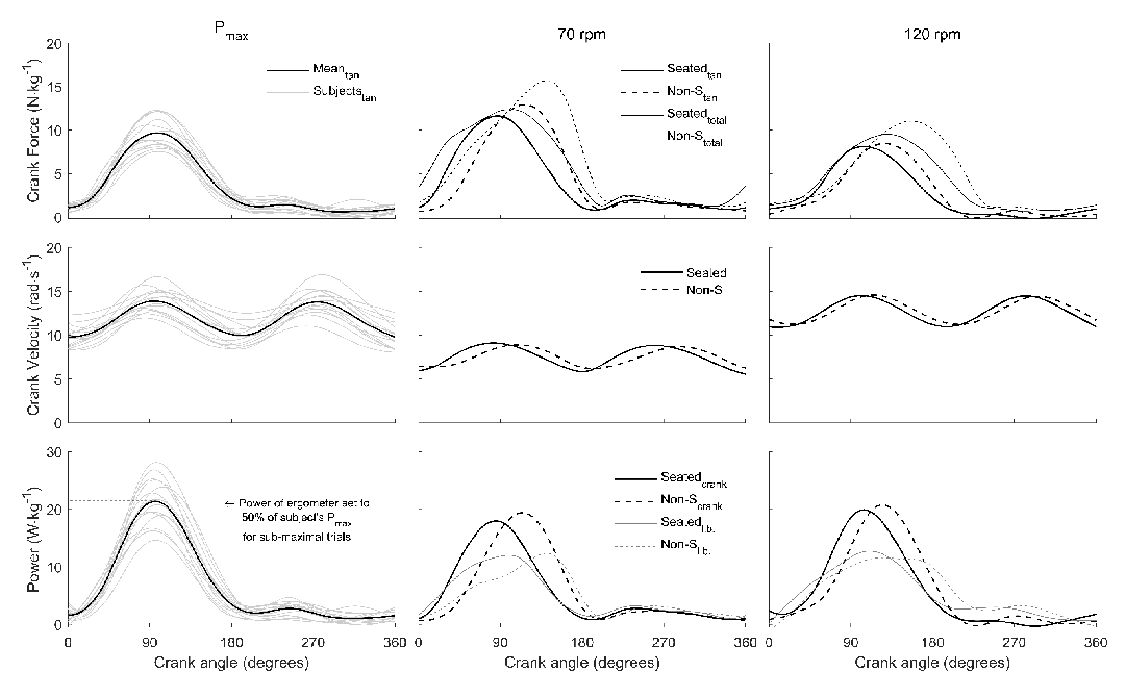
\includegraphics[width=0.9\textwidth]{SupplementaryFigures/Study1_supp1.eps}
    \caption[Peak crank power far exceeds peak power generated by the leg during seated and non-seated cycling, suggesting that additional power is generated by muscles in the upper body or or the rider's CoM.]{\textbf{Peak crank power far exceeds peak power generated by the leg during seated and non-seated cycling, suggesting that additional power is generated by muscles in the upper body or or the rider's CoM.} Participant and group mean crank force, velocity and power during the P$_{max.i}$ trials (left column) as well as a comparison of crank and leg power during the sub-maximal trials at 70 rpm (centre) and 120 rpm (right).}
    \label{fig:m1sdc1}
\end{sidewaysfigure}

\begin{table}[htbp]
    \centering
    \ra{1.3}
    \begin{tabular}{@{}l*5{r}@{}}
        \toprule
         & \multicolumn{2}{c}{70 rpm} && \multicolumn{2}{c}{120 rpm} \\
         \cmidrule{2-3} \cmidrule{5-6}
         & \multicolumn{1}{c}{Seated} & \multicolumn{1}{c}{Non-seated} && \multicolumn{1}{c}{Seated} & \multicolumn{1}{c}{Non-seated} \\
         \midrule
        Peak hip extension \\
        \hspace{0.5cm}angle (deg) & $43\pm5^{p}$ & $30\pm5$ && $42\pm5^{p}$ & $32\pm5$ \\
        \hspace{0.5cm}velocity (deg/s) & $-177\pm34^{c}$ & $-167\pm26^{c}$ && $-328\pm36$ & $-315\pm38$ \\
        \hspace{0.5cm}moment (Nm/kg) & $-3.7\pm0.5^{p,c}$ & $-4.3\pm0.7^{c}$ && $-3.0\pm0.5$ & $-3.1\pm0.6$ \\
        \hdashline
        Peak hip flexion \\
        \hspace{0.5cm}angle (deg) & $89\pm6^{p}$ & $79\pm4^{c}$ && $92\pm5^{p}$ & $84\pm4$ \\
        \hspace{0.5cm}velocity (deg/s) & $155\pm33^{c}$ & $185\pm35^{c}$ && $259\pm33^{p}$ & $294\pm36$ \\
        \hspace{0.5cm}moment (Nm/kg) & $1.1\pm0.4^{c}$ & $1.0\pm0.3$ && $-0.8\pm0.3$ & $1.0\pm0.2$ \\
        \hdashline
        Peak knee extension \\
        \hspace{0.5cm}angle (deg) & $23\pm6^{p,c}$ & $14\pm3$ && $33\pm6^{p}$ & $21\pm5$ \\
        \hspace{0.5cm}velocity (deg/s) & $-294\pm28^{c}$ & $-295\pm24^{c}$ && $-507\pm53^{p}$ & $548\pm42$ \\
        \hspace{0.5cm}moment (Nm/kg) & $-1.5\pm0.4^{p,c}$ & $-1.2\pm0.4^{c}$ && $-0.8\pm0.1$ & $-0.8\pm0.1$ \\
        \hdashline
        Peak knee flexion \\
        \hspace{0.5cm}angle (deg) & $109\pm3^{c}$ & $109\pm3$ && $114\pm2^{p}$ & $109\pm3$ \\
        \hspace{0.5cm}velocity (deg/s) & $324\pm56^{p,c}$ & $417\pm43^{c}$ && $497\pm46$ & $520\pm38$ \\
        \hspace{0.5cm}moment (Nm/kg) & $1.7\pm0.3$ & $1.6\pm0.3$ && $1.5\pm0.2$ & $1.7\pm0.3$ \\
        \hdashline
        Peak ankle plantar flexion \\
        \hspace{0.5cm}angle (deg) & $-26\pm9^{p,c}$ & $-32\pm5^{c}$ && $-20\pm8^{p}$ & $-26\pm7$ \\
        \hspace{0.5cm}velocity (deg/s) & $-240\pm33^{p}$ & $-316\pm55$ && $-251\pm65$ & $-259\pm54$ \\
        \hspace{0.5cm}moment (Nm/kg) & $-1.5\pm0.2^{p,c}$ & $-2.0\pm0.2^{c}$ && $-1.2\pm0.3^{p}$ & $1.4\pm0.3$ \\
        \hdashline
        Peak ankle dorsiflexion \\
        \hspace{0.5cm}angle (deg) & $25\pm5^{p,c}$ & $20\pm5^{c}$ && $11\pm6$ & $9\pm6$ \\
        \hspace{0.5cm}velocity (deg/s) & $282\pm91^{p}$ & $209\pm60$ && $237\pm77$ & $265\pm66$ \\
        \hspace{0.5cm}moment (Nm/kg) & $0.2\pm0.1^{c}$ & $0.2\pm0.1^{c}$ && $0.1\pm0.1$ & $0.2\pm0.1$ \\
         \bottomrule
         \multicolumn{6}{l}{$^p$Statistically significant difference to Non-seated within cadence ($P<0.037$).} \\
         \multicolumn{6}{l}{$^c$Statistically significant difference to 120 rpm within posture ($P<0.037$).} \\
    \end{tabular}
    \caption[When non-seated at 70 rpm, peak-knee-extension moments decreased, while range of motion at the knee increased compared to seated.]{\textbf{When non-seated at 70 rpm, peak-knee-extension moments decreased, while range of motion at the knee increased compared to seated.} Group mean ($\pm$SD) peak angle, peak velocity, and peak joint moments at the hip, knee, and ankle during high-power-output cycling ($10.7\pm2.0$ W/kg) at low (70 rpm) and high (120 rpm) cadence ($n=15$).}
    \label{tab:m1sdc2}
\end{table}

\begin{figure}
    \centering
    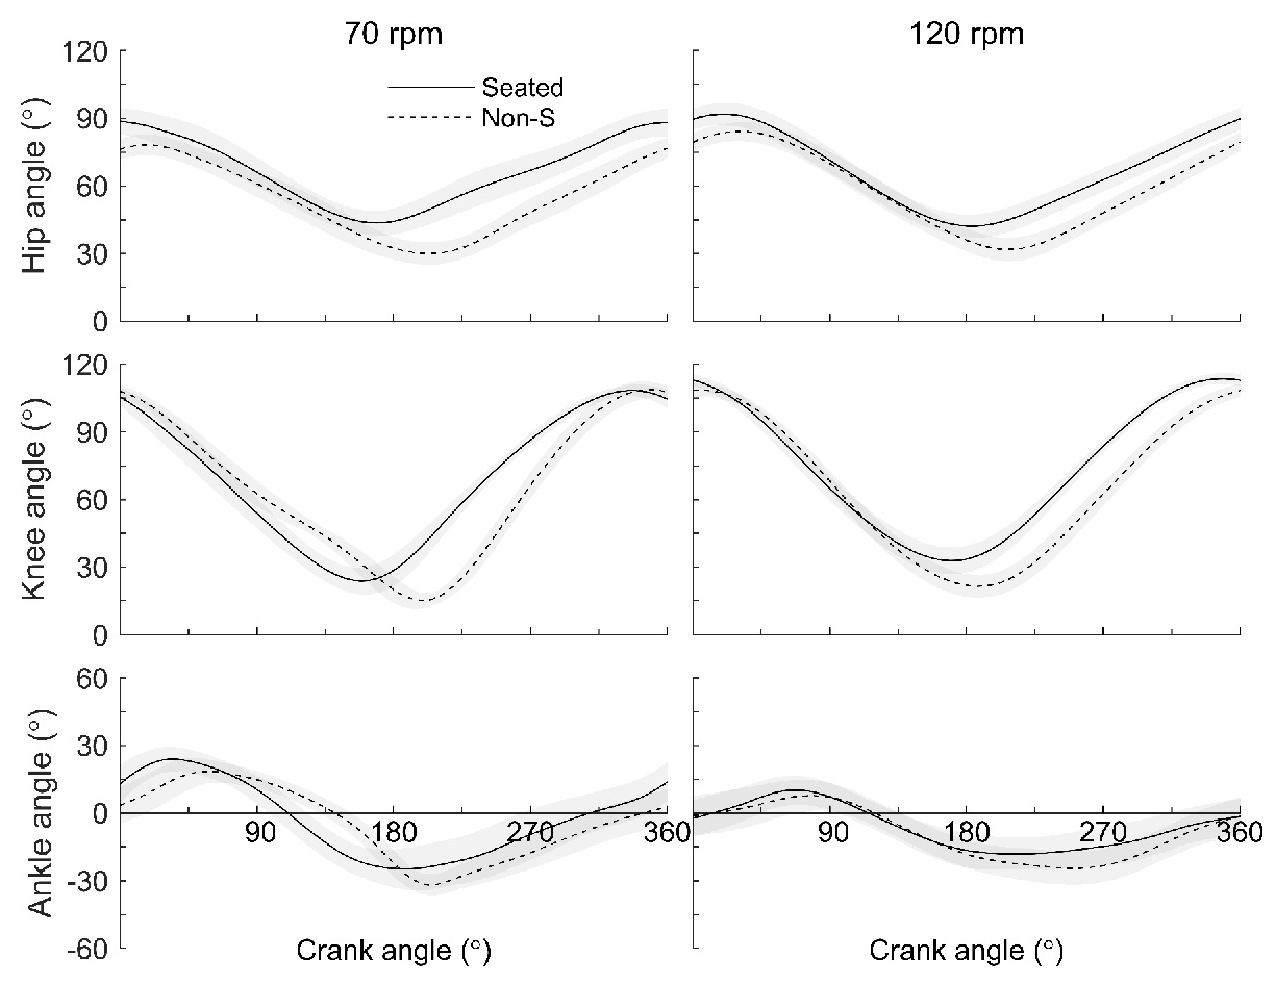
\includegraphics[width=\textwidth]{SupplementaryFigures/Study1_supp3.eps}
    \caption[The hip, knee, and ankle extend later in the crank cycle and to a greater extent when non-seated compared to when seated.]{\textbf{The hip, knee, and ankle extend later in the crank cycle and to a greater extent when non-seated compared to when seated.} Group mean ($\pm$SD, shaded area) joint angle with respect to crank angle at the hip, knee and ankle during each condition.}
    \label{fig:m1sdc3}
\end{figure}

\begin{figure}
    \centering
    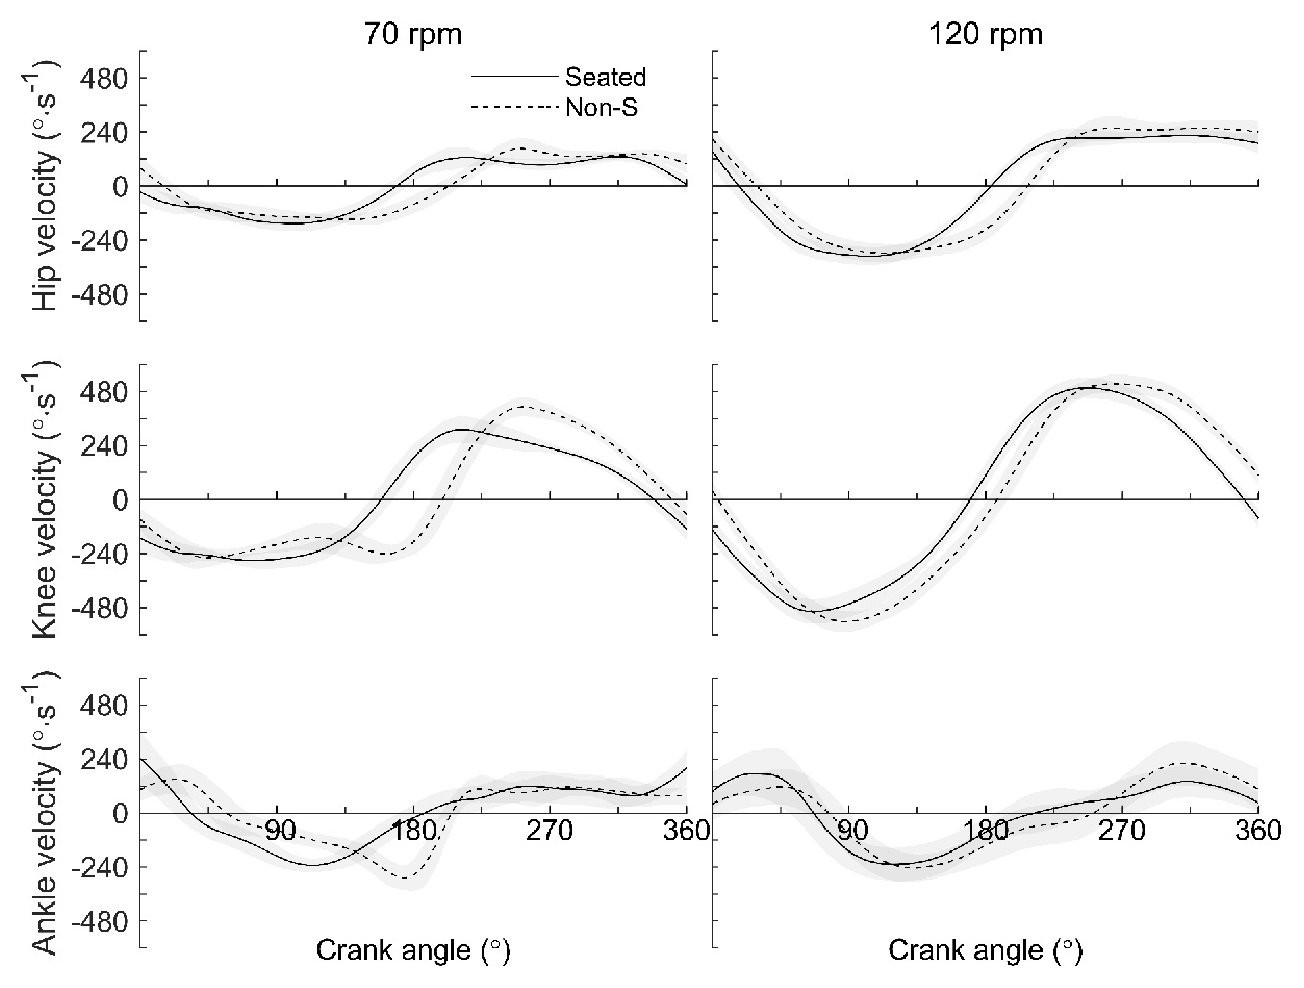
\includegraphics[width=\textwidth]{SupplementaryFigures/Study1_supp4.eps}
    \caption[Duty cycle of the knee increased at 70 rpm when non-seated compared to when seated, which also resulted in greater peak knee flexion velocity.]{\textbf{Duty cycle of the knee increased at 70 rpm when non-seated compared to when seated, which also resulted in greater peak knee flexion velocity.} Group mean ($\pm$SD, shaded area) joint velocity with respect to crank angle at the hip, knee and ankle during each condition.}
    \label{fig:m1sdc4}
\end{figure}

\begin{figure}
    \centering
    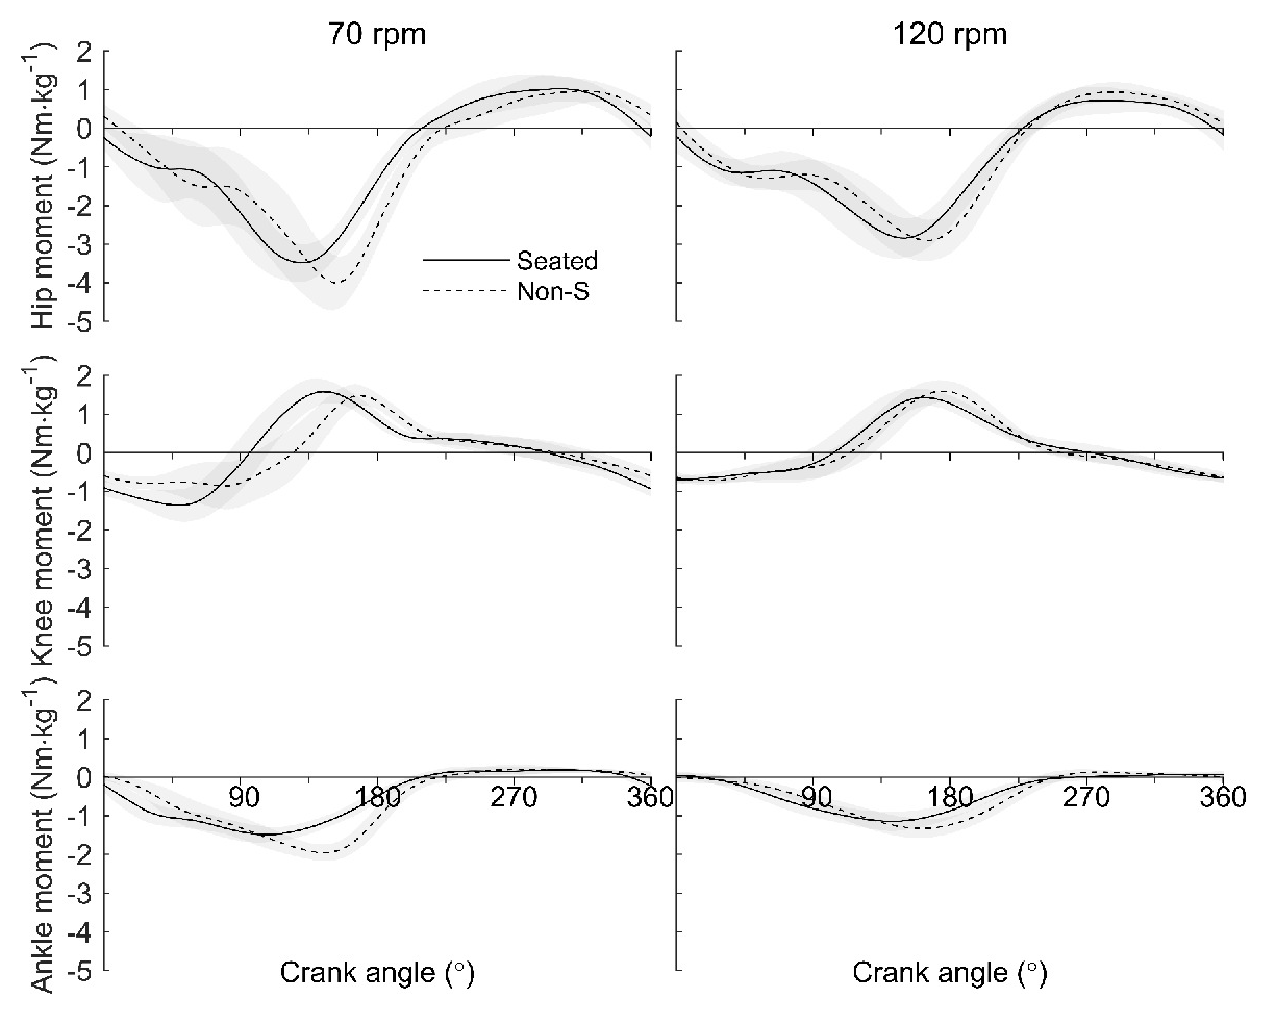
\includegraphics[width=\textwidth]{SupplementaryFigures/Study1_supp5.eps}
    \caption[Peak hip extension moments and ankle plantar flexion moments increased when non-seated at 70 rpm, likely due to an increased redistribution of net joint moments by bi-articular muscles.]{\textbf{Peak hip extension moments and ankle plantar flexion moments increased when non-seated at 70 rpm, likely due to an increased redistribution of net joint moments by bi-articular muscles.} Group mean ($\pm$SD, shaded area) net joint moments with respect to crank angle at the hip, knee and ankle during each condition.}
    \label{fig:m1sdc5}
\end{figure}

\begin{figure}
    \centering
    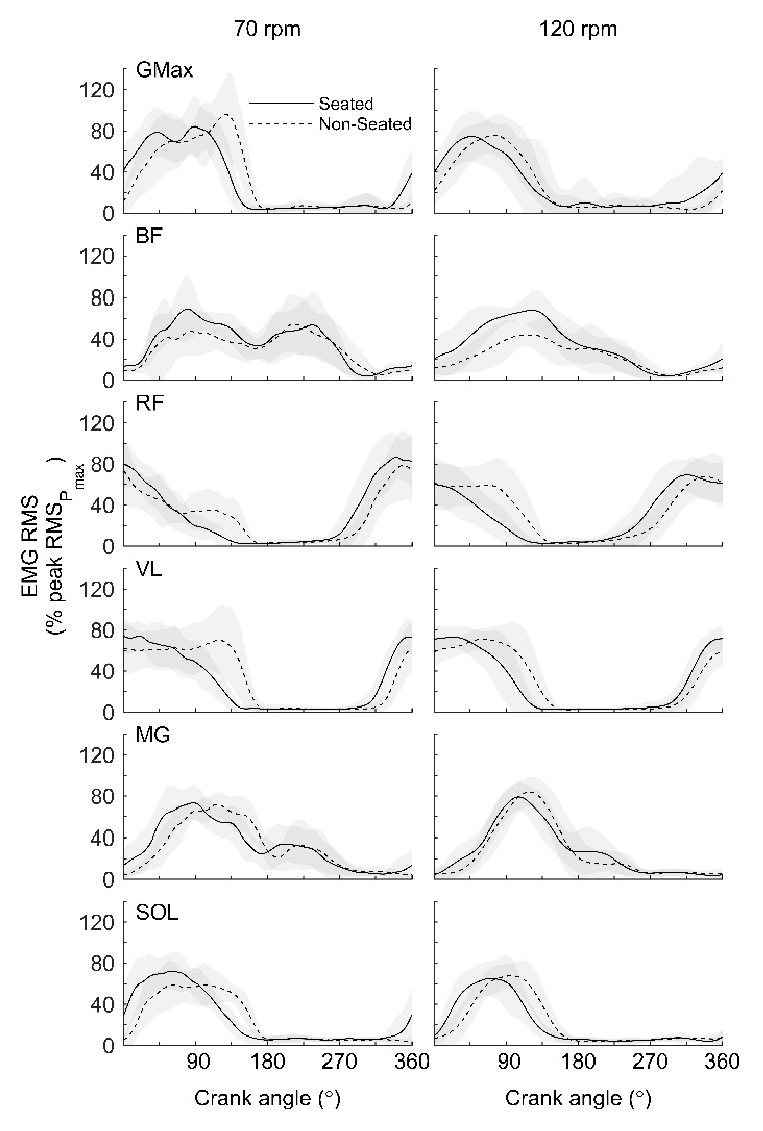
\includegraphics[width=0.85\textwidth]{SupplementaryFigures/Study1_supp6.eps}
    \caption[The period of EMG activity of most muscles within the lower limb was shifted later in the crank cycle when cycling in a non-seated posture.]{\textbf{The period of EMG activity of most muscles within the lower limb was shifted later in the crank cycle when cycling in a non-seated posture.} Group mean ($\pm$SD, shaded area) EMG activity of muscles within the right lower limb with respect to crank angle during high-power output cycling at 70 rpm and 120 rpm in a seated and non-seated posture.}
    \label{fig:m1sdc6}
\end{figure}
\FloatBarrier

\section{Supplementary figure for study in Chapter 4}

\begin{figure}[htbp]
    \centering
    \includegraphics[width=\textwidth]{SupplementaryFigures/Study2_supp1.png}
    \caption[Rider CoM displacement occurred predominantly in the vertical direction during non-seated cycling.]{\textbf{Rider CoM displacement occurred predominantly in the vertical direction during non-seated cycling.} Data in the cubes show the group mean CoM trajectory (green) projected onto  three planes (black) during non-seated cycling under different power outputs (10$\%$, 30$\%$, and 50$\%$ P$_{max.i}$) at 70 rpm (left) and 120 rpm (right). The X, Y, and Z axes relate to CoM movement in the anterior-posterior, medio-lateral and vertical directions, respectively. Cartesian plots show the group mean CoM vertical displacement, velocity and acceleration with respect to crank angle (0\textdegree; top dead centre) under the same conditions. Note that displacement is the result of work done on, or by, the CoM. Velocity is the result of power generated on, or by, the CoM. Acceleration is the result of vertical interaction force between the bicycle and the rider.}
    \label{fig:m2f2}
\end{figure}
\FloatBarrier
\clearpage

\section{Supplementary figures for study in Chapter 5}

\begin{figure}[htbp]
    \centering
    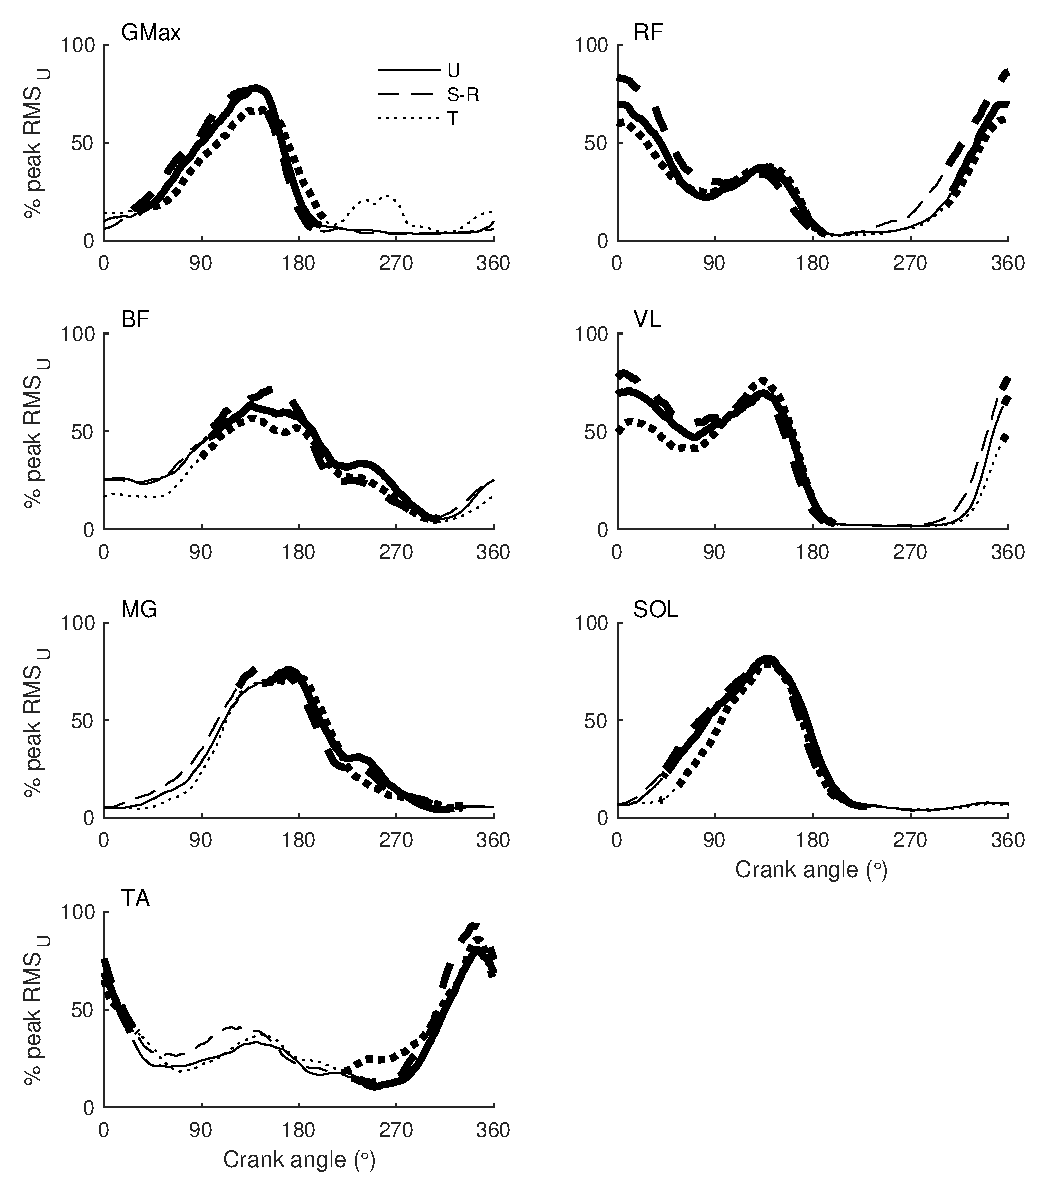
\includegraphics[width=\textwidth]{SupplementaryFigures/Study3_supp2.eps}
    \caption[On average, the mean EMG RMS activity of GMax, VL, and SOL were lower in the Trainer condition compared to Unconstrained and Self-Restricted.]{\textbf{On average, the mean EMG RMS activity of GMax, VL, and SOL were lower in the Trainer condition compared to Unconstrained and Self-Restricted.} Group mean ($n=11$) EMG activity of seven muscles in the right leg across the crank cycle with respect to the peak level of activity in the Unconstrained condition. The period of shortening in each respective MTU is indicated by the thicker lines.}
    \label{fig:m3_sdc2}
\end{figure}

\begin{figure}[htbp]
    \centering
    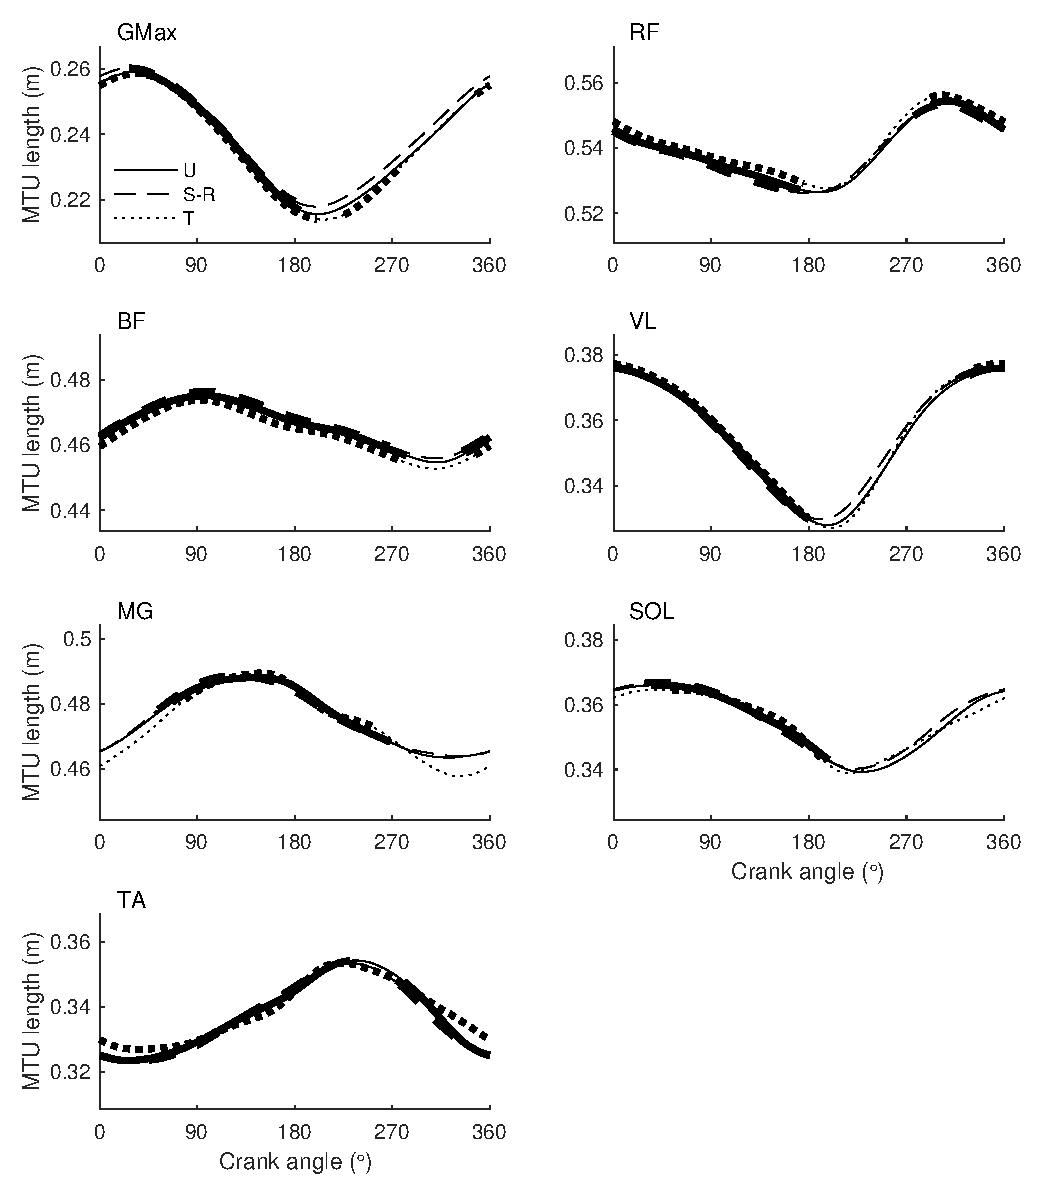
\includegraphics[width=\textwidth]{SupplementaryFigures/Study3_supp3.eps}
    \caption[MTU lengths in the Self-Restricted and Trainer conditions appear to subtly diverge from Unconstrained.]{\textbf{MTU lengths in the Self-Restricted and Trainer conditions appear to subtly diverge from Unconstrained.}Group mean MTU lengths of seven muscles in the right leg across the crank cycle during non-seated cycling at $5$ W$\cdot$kg$^{-1}$ and 70 rpm ($n=11$). The period of EMG activity of each respective muscle is indicated by the thicker lines.}
    \label{fig:m3_sdc3}
\end{figure}

\begin{sidewaysfigure}[htbp]
    \centering
    \includegraphics[width=0.9\textwidth]{SupplementaryFigures/Study3_supp1.png}
    \caption[Riders appeared to dissipate power at the knee much earlier in the crank cycle when self-restricting bicycle lean.]{\textbf{Riders appeared to dissipate power at the knee much earlier in the crank cycle when self-restricting bicycle lean.} Group mean net joint moments, joint velocities, and joint power at the hip, knee, ankle in each condition. The altered pattern of power generation and dissipation within the right lower limb in the self-restricted condition points toward a greater demand on bi-articular knee extensors and flexors to transfer power from the knee to hip and ankle during the downstroke.}
    \label{fig:m3_sdc1}    
\end{sidewaysfigure}

\begin{sidewaysfigure}[htbp]
    \centering
    \includegraphics[width=0.9\textwidth]{SupplementaryFigures/Study3_supp4.pdf}
    \caption[Technical drawing of instrumented cranks used for study in Chapter \ref{Chap:5}.]{\textbf{Technical drawing of instrumented cranks used for study in Chapter \ref{Chap:5}.}} \label{fig:m3_sdc4}
\end{sidewaysfigure}
 % Supplementary Figures

%% *************** APPENDIX F ***************
\cleartoevenpage
\pagestyle{empty}	%Use this to suppress the header from the preceding chapter.

\chapter{Ethical Approval Forms}
\label{Chap:F}
\pagestyle{headings}

\includepdf[scale=0.8, offset=0 -1cm, pages=-, pagecommand=\section{Ethical approval for studies in Chapters 3 and 4, and Appendix B} \label{sec:F1}]{EthicsForms/Form1.pdf}

\includepdf[scale=0.8, offset=0 -1cm, pages=-, pagecommand=\section{Ethical approval for study in Chapter 5} \label{sec:F2}]{EthicsForms/Form2.pdf}

\includepdf[scale=0.8, offset=0 -1cm, pages=-, pagecommand=\section{Ethical approval for studies in Appendix C and D} \label{sec:F3}]{EthicsForms/Form3.pdf} % Ethical Forms

%% *************** APPENDIX G ***************
\cleartooddpage[\vspace*{\fill}\begin{center} This page intentionally left blank. \end{center} \vspace*{\fill}]
\chapter{Copyright Permissions}
\label{Chap:G}

\includepdf[scale=0.8, pages={1}, pagecommand=\section{Copyright permission for Figure 2.1} \label{sec:G1}]{CopyrightPermissions/CC_FigureLi.pdf}

\includepdf[scale=0.8, pages={1}, pagecommand=\section{Copyright permission for Figure 2.2} \label{sec:G2}]{CopyrightPermissions/CC_FigureZajac.pdf}

\includepdf[scale=0.8, pages={1}, pagecommand=\section{Copyright permission for Figure 2.3} \label{sec:G2}]{CopyrightPermissions/CC_FigureKipp.pdf}

\includepdf[scale=0.8, pages={1}, pagecommand=\section{Copyright permission for Figure 2.4} \label{sec:G3}]{CopyrightPermissions/CC_FigureElmer.pdf}

\includepdf[scale=0.8, pages={1}, pagecommand=\section{Copyright permission for Figure 2.5} \label{sec:G4}]{CopyrightPermissions/CC_FigureHull.pdf} % Copyright Permissions


% *************** Back matter ***************
%COMMENT OUT IF YOU DO NOT WISH TO INCLUDE BACK MATTER.
cs% *************** Back matter ***************
\backmatter

\normalfont

% *************** End of back matter ***************
% ADD AN ENDQUOTE HERE. If you do not wish to, delete this file.
\cleartooddpage

\pagestyle{empty}

\begin{table}[b!]
\begin{center}
\textit{When the spirits are low, when the day appears dark, when work becomes monotonous, when hope hardly seems worth having, just mount a bicycle and go out for a spin down the road, without thought on anything but the ride you are taking}
\end{center}
\begin{flushright}
Sir Arthur Conan Doyle,\\
Scientific American, Volume 74, January 18, 1896.
\end{flushright}
\end{table}

\end{document}